\begin{appendices}

    % -------------------------------
    % -------------------------------
    % ------- BAYSIS Appendix -------
    % -------------------------------
    % -------------------------------
    \chapter{BAYSIS Figures and Tables}
    \label{appendix_baysis}
    
    % --------------------------------
    % ------- BAYSIS Dataset ---------
    % --------------------------------
    \tocless\section{BAYSIS Data Foundation}
    \label{appendix_baysis_dataset}
    
    % ------- BAYSIS Dataset - Figures --------
    
    % ------- BAYSIS Dataset - Tables --------
    \newgeometry{left=1cm,right=1cm,top=1cm}
    \begin{sidewaystable}
    \tiny
    \setlength{\tabcolsep}{4pt}
    \centering
    \begin{tabular}{lrrrrrrrrrrrrrrrrrrrr}
\toprule
{} &  Strasse &  Kat &  Typ &  Betei &  UArt1 &  UArt2 &  AUrs1 &  AUrs2 &  AufHi &  Alkoh &  Char1 &  Char2 &  Lich1 &  Lich2 &  Zust1 &  Zust2 &  Fstf &  WoTag &  FeiTag &  Month \\
\midrule
Strasse &     1.00 & 0.07 & 0.11 &   0.08 &   0.09 &   0.05 &   0.07 &   0.04 &   0.08 &   0.07 &   0.12 &   0.10 &   0.05 &   0.06 &   0.10 &   0.06 &  0.15 &   0.09 &    0.05 &   0.05 \\
Kat     &     0.07 & 1.00 & 0.16 &   0.18 &   0.31 &   0.10 &   0.08 &   0.05 &   0.12 &   0.02 &   0.05 &   0.03 &   0.02 &   0.04 &   0.05 &   0.02 &  0.08 &   0.04 &    0.03 &   0.05 \\
Typ     &     0.11 & 0.16 & 1.00 &   0.31 &   0.56 &   0.06 &   0.26 &   0.06 &   0.25 &   0.06 &   0.15 &   0.09 &   0.09 &   0.20 &   0.33 &   0.12 &  0.16 &   0.08 &    0.05 &   0.09 \\
Betei   &     0.08 & 0.18 & 0.31 &   1.00 &   0.28 &   0.06 &   0.14 &   0.20 &   0.24 &   0.04 &   0.07 &   0.07 &   0.09 &   0.09 &   0.25 &   0.10 &  0.08 &   0.07 &    0.06 &   0.06 \\
UArt1   &     0.09 & 0.31 & 0.56 &   0.28 &   1.00 &   0.08 &   0.21 &   0.05 &   0.32 &   0.05 &   0.14 &   0.09 &   0.10 &   0.22 &   0.25 &   0.09 &  0.16 &   0.08 &    0.05 &   0.06 \\
UArt2   &     0.05 & 0.10 & 0.06 &   0.06 &   0.08 &   1.00 &   0.06 &   0.03 &   0.15 &   0.04 &   0.03 &   0.05 &   0.03 &   0.05 &   0.08 &   0.04 &  0.04 &   0.04 &    0.01 &   0.04 \\
AUrs1   &     0.07 & 0.08 & 0.26 &   0.14 &   0.21 &   0.06 &   1.00 &   0.20 &   0.16 &   0.05 &   0.08 &   0.09 &   0.12 &   0.13 &   0.66 &   0.77 &  0.05 &   0.09 &    0.04 &   0.15 \\
AUrs2   &     0.04 & 0.05 & 0.06 &   0.20 &   0.05 &   0.03 &   0.20 &   1.00 &   0.06 &   0.04 &   0.03 &   0.06 &   0.04 &   0.03 &   0.12 &   0.33 &  0.03 &   0.03 &    0.03 &   0.05 \\
AufHi   &     0.08 & 0.12 & 0.25 &   0.24 &   0.32 &   0.15 &   0.16 &   0.06 &   1.00 &   0.04 &   0.08 &   0.10 &   0.08 &   0.10 &   0.25 &   0.09 &  0.06 &   0.07 &    0.04 &   0.06 \\
Alkoh   &     0.07 & 0.02 & 0.06 &   0.04 &   0.05 &   0.04 &   0.05 &   0.04 &   0.04 &   1.00 &   0.02 &   0.00 &   0.11 &   0.11 &   0.03 &   0.01 &  0.05 &   0.08 &    0.01 &   0.05 \\
Char1   &     0.12 & 0.05 & 0.15 &   0.07 &   0.14 &   0.03 &   0.08 &   0.03 &   0.08 &   0.02 &   1.00 &   0.58 &   0.04 &   0.05 &   0.10 &   0.03 &  0.06 &   0.03 &    0.02 &   0.04 \\
Char2   &     0.10 & 0.03 & 0.09 &   0.07 &   0.09 &   0.05 &   0.09 &   0.06 &   0.10 &   0.00 &   0.58 &   1.00 &   0.04 &   0.04 &   0.08 &   0.03 &  0.08 &   0.03 &    0.02 &   0.04 \\
Lich1   &     0.05 & 0.02 & 0.09 &   0.09 &   0.10 &   0.03 &   0.12 &   0.04 &   0.08 &   0.11 &   0.04 &   0.04 &   1.00 &   0.71 &   0.16 &   0.06 &  0.05 &   0.04 &    0.03 &   0.21 \\
Lich2   &     0.06 & 0.04 & 0.20 &   0.09 &   0.22 &   0.05 &   0.13 &   0.03 &   0.10 &   0.11 &   0.05 &   0.04 &   0.71 &   1.00 &   0.16 &   0.06 &  0.17 &   0.04 &    0.03 &   0.20 \\
Zust1   &     0.10 & 0.05 & 0.33 &   0.25 &   0.25 &   0.08 &   0.66 &   0.12 &   0.25 &   0.03 &   0.10 &   0.08 &   0.16 &   0.16 &   1.00 &   0.17 &  0.06 &   0.12 &    0.05 &   0.37 \\
Zust2   &     0.06 & 0.02 & 0.12 &   0.10 &   0.09 &   0.04 &   0.77 &   0.33 &   0.09 &   0.01 &   0.03 &   0.03 &   0.06 &   0.06 &   0.17 &   1.00 &  0.05 &   0.06 &    0.02 &   0.17 \\
Fstf    &     0.15 & 0.08 & 0.16 &   0.08 &   0.16 &   0.04 &   0.05 &   0.03 &   0.06 &   0.05 &   0.06 &   0.08 &   0.05 &   0.17 &   0.06 &   0.05 &  1.00 &   0.03 &    0.02 &   0.04 \\
WoTag   &     0.09 & 0.04 & 0.08 &   0.07 &   0.08 &   0.04 &   0.09 &   0.03 &   0.07 &   0.08 &   0.03 &   0.03 &   0.04 &   0.04 &   0.12 &   0.06 &  0.03 &   1.00 &    0.13 &   0.09 \\
FeiTag  &     0.05 & 0.03 & 0.05 &   0.06 &   0.05 &   0.01 &   0.04 &   0.03 &   0.04 &   0.01 &   0.02 &   0.02 &   0.03 &   0.03 &   0.05 &   0.02 &  0.02 &   0.13 &    1.00 &   0.13 \\
Month   &     0.05 & 0.05 & 0.09 &   0.06 &   0.06 &   0.04 &   0.15 &   0.05 &   0.06 &   0.05 &   0.04 &   0.04 &   0.21 &   0.20 &   0.37 &   0.17 &  0.04 &   0.09 &    0.13 &   1.00 \\
\bottomrule
\end{tabular}

    \caption{Correlation matrix for BAYSIS dataset, with Cramer's $V$}
    \label{table:appendix_correlation_matrix_dataset_cramers}
    \end{sidewaystable}
    
    \begin{sidewaystable}
    \tiny
    \setlength{\tabcolsep}{4pt}
    \centering
    \begin{tabular}{lrrrrrrrrrrrrrrrrrrrrrr}
\toprule
{} &  Strasse &  Kat &  Typ &  Betei &  UArt1 &  UArt2 &  AUrs1 &  AUrs2 &  AufHi &  Alkoh &  Char1 &  Char2 &  Bes1 &  Bes2 &  Lich1 &  Lich2 &  Zust1 &  Zust2 &  Fstf &  WoTag &  FeiTag &  Month \\
\midrule
Strasse &     1.00 & 0.00 & 0.02 &   0.01 &   0.01 &   0.00 &   0.01 &   0.00 &   0.01 &   0.00 &   0.01 &   0.00 &  0.01 &  0.00 &   0.00 &   0.00 &   0.00 &   0.00 &  0.04 &   0.01 &    0.00 &   0.01 \\
Kat     &     0.01 & 1.00 & 0.04 &   0.05 &   0.16 &   0.02 &   0.01 &   0.00 &   0.01 &   0.00 &   0.00 &   0.00 &  0.00 &  0.00 &   0.00 &   0.00 &   0.00 &   0.00 &  0.01 &   0.00 &    0.00 &   0.00 \\
Typ     &     0.03 & 0.03 & 1.00 &   0.26 &   0.39 &   0.01 &   0.15 &   0.01 &   0.17 &   0.00 &   0.02 &   0.00 &  0.02 &  0.00 &   0.01 &   0.02 &   0.09 &   0.01 &  0.05 &   0.02 &    0.00 &   0.02 \\
Betei   &     0.02 & 0.04 & 0.29 &   1.00 &   0.36 &   0.01 &   0.09 &   0.01 &   0.22 &   0.00 &   0.01 &   0.00 &  0.01 &  0.00 &   0.01 &   0.01 &   0.05 &   0.01 &  0.02 &   0.02 &    0.00 &   0.01 \\
UArt1   &     0.02 & 0.07 & 0.25 &   0.20 &   1.00 &   0.02 &   0.07 &   0.00 &   0.25 &   0.00 &   0.01 &   0.00 &  0.01 &  0.00 &   0.01 &   0.01 &   0.03 &   0.00 &  0.05 &   0.01 &    0.00 &   0.01 \\
UArt2   &     0.02 & 0.03 & 0.02 &   0.03 &   0.07 &   1.00 &   0.02 &   0.00 &   0.20 &   0.00 &   0.01 &   0.00 &  0.01 &  0.00 &   0.00 &   0.01 &   0.01 &   0.00 &  0.01 &   0.01 &    0.00 &   0.01 \\
AUrs1   &     0.05 & 0.01 & 0.25 &   0.14 &   0.18 &   0.01 &   1.00 &   0.04 &   0.14 &   0.00 &   0.02 &   0.01 &  0.03 &  0.00 &   0.02 &   0.02 &   0.38 &   0.05 &  0.01 &   0.03 &    0.00 &   0.14 \\
AUrs2   &     0.09 & 0.02 & 0.12 &   0.10 &   0.12 &   0.02 &   0.37 &   1.00 &   0.08 &   0.01 &   0.02 &   0.01 &  0.02 &  0.00 &   0.02 &   0.01 &   0.16 &   0.25 &  0.05 &   0.05 &    0.01 &   0.13 \\
AufHi   &     0.03 & 0.01 & 0.22 &   0.25 &   0.50 &   0.11 &   0.11 &   0.01 &   1.00 &   0.00 &   0.02 &   0.01 &  0.02 &  0.00 &   0.01 &   0.01 &   0.07 &   0.01 &  0.02 &   0.02 &    0.00 &   0.02 \\
Alkoh   &     0.01 & 0.00 & 0.01 &   0.01 &   0.02 &   0.01 &   0.02 &   0.00 &   0.01 &   1.00 &   0.00 &   0.00 &  0.00 &  0.00 &   0.05 &   0.05 &   0.00 &   0.00 &  0.01 &   0.03 &    0.00 &   0.01 \\
Char1   &     0.06 & 0.01 & 0.05 &   0.03 &   0.05 &   0.01 &   0.03 &   0.00 &   0.03 &   0.00 &   1.00 &   0.14 &  0.00 &  0.00 &   0.00 &   0.00 &   0.02 &   0.00 &  0.02 &   0.01 &    0.00 &   0.01 \\
Char2   &     0.05 & 0.00 & 0.03 &   0.02 &   0.03 &   0.01 &   0.03 &   0.01 &   0.04 &   0.00 &   0.60 &   1.00 &  0.01 &  0.00 &   0.01 &   0.01 &   0.03 &   0.00 &  0.02 &   0.00 &    0.00 &   0.01 \\
Bes1    &     0.07 & 0.01 & 0.05 &   0.02 &   0.06 &   0.01 &   0.05 &   0.00 &   0.05 &   0.00 &   0.01 &   0.00 &  1.00 &  0.01 &   0.00 &   0.00 &   0.03 &   0.00 &  0.03 &   0.01 &    0.00 &   0.03 \\
Bes2    &     0.13 & 0.01 & 0.05 &   0.10 &   0.08 &   0.01 &   0.11 &   0.00 &   0.06 &   0.00 &   0.03 &   0.00 &  0.73 &  1.00 &   0.03 &   0.02 &   0.01 &   0.00 &  0.05 &   0.08 &    0.00 &   0.09 \\
Lich1   &     0.00 & 0.00 & 0.01 &   0.01 &   0.01 &   0.00 &   0.02 &   0.00 &   0.01 &   0.01 &   0.00 &   0.00 &  0.00 &  0.00 &   1.00 &   0.80 &   0.03 &   0.00 &  0.00 &   0.00 &    0.00 &   0.06 \\
Lich2   &     0.01 & 0.00 & 0.03 &   0.01 &   0.04 &   0.00 &   0.02 &   0.00 &   0.02 &   0.01 &   0.00 &   0.00 &  0.00 &  0.00 &   0.90 &   1.00 &   0.04 &   0.00 &  0.03 &   0.00 &    0.00 &   0.06 \\
Zust1   &     0.01 & 0.00 & 0.14 &   0.08 &   0.08 &   0.01 &   0.36 &   0.02 &   0.08 &   0.00 &   0.01 &   0.00 &  0.01 &  0.00 &   0.03 &   0.03 &   1.00 &   0.04 &  0.00 &   0.02 &    0.00 &   0.14 \\
Zust2   &     0.03 & 0.01 & 0.13 &   0.08 &   0.07 &   0.01 &   0.38 &   0.19 &   0.08 &   0.00 &   0.01 &   0.00 &  0.02 &  0.00 &   0.03 &   0.03 &   0.28 &   1.00 &  0.02 &   0.02 &    0.00 &   0.24 \\
Fstf    &     0.06 & 0.01 & 0.04 &   0.02 &   0.06 &   0.00 &   0.01 &   0.00 &   0.01 &   0.00 &   0.01 &   0.00 &  0.01 &  0.00 &   0.00 &   0.01 &   0.00 &   0.00 &  1.00 &   0.00 &    0.00 &   0.00 \\
WoTag   &     0.01 & 0.00 & 0.01 &   0.01 &   0.01 &   0.00 &   0.01 &   0.00 &   0.01 &   0.00 &   0.00 &   0.00 &  0.00 &  0.00 &   0.00 &   0.00 &   0.01 &   0.00 &  0.00 &   1.00 &    0.00 &   0.01 \\
FeiTag  &     0.01 & 0.00 & 0.01 &   0.01 &   0.01 &   0.00 &   0.01 &   0.00 &   0.01 &   0.00 &   0.00 &   0.00 &  0.00 &  0.00 &   0.00 &   0.00 &   0.01 &   0.00 &  0.00 &   0.07 &    1.00 &   0.10 \\
Month   &     0.01 & 0.00 & 0.01 &   0.01 &   0.01 &   0.00 &   0.04 &   0.00 &   0.01 &   0.00 &   0.00 &   0.00 &  0.00 &  0.00 &   0.02 &   0.02 &   0.04 &   0.01 &  0.00 &   0.01 &    0.00 &   1.00 \\
\bottomrule
\end{tabular}

    \caption{Correlation matrix for BAYSIS dataset, with Theil's $U$}
    \label{table:appendix_correlation_matrix_dataset_theils}
    \end{sidewaystable}
    
    \begin{sidewaystable}
    \tiny
    \setlength{\tabcolsep}{4pt}
    \centering
    \begin{tabular}{lrrrrrrrrrrrrrrrrrrrrrrr}
\toprule
{} &  Strasse &   Kat &   Typ &  Betei &  UArt1 &  UArt2 &  AUrs1 &  AUrs2 &  AufHi &  Alkoh &  Char1 &  Char2 &  Bes1 &  Bes2 &  Lich1 &  Lich2 &  Zust1 &  Zust2 &  Fstf &  StrklVu &  WoTag &  FeiTag &  Month \\
\midrule
Strasse &      nan & 0.000 & 0.000 &  0.000 &  0.000 &  0.000 &  0.000 &  0.871 &  0.000 &  0.000 &  0.000 &  0.000 & 0.000 & 0.357 &  0.165 &  0.000 &  0.000 &  0.006 & 0.000 &    0.870 &  0.000 &   0.073 &  0.002 \\
Kat     &    0.000 &   nan & 0.000 &  0.000 &  0.000 &  0.000 &  0.000 &  0.000 &  0.000 &  0.225 &  0.000 &  0.058 & 0.000 & 0.754 &  0.260 &  0.000 &  0.000 &  0.068 & 0.000 &    0.760 &  0.000 &   0.069 &  0.000 \\
Typ     &    0.000 & 0.000 &   nan &  0.000 &  0.000 &  0.000 &  0.000 &  0.000 &  0.000 &  0.000 &  0.000 &  0.000 & 0.000 & 0.691 &  0.000 &  0.000 &  0.000 &  0.000 & 0.000 &    0.000 &  0.000 &   0.000 &  0.000 \\
Betei   &    0.000 & 0.000 & 0.000 &    nan &  0.000 &  0.000 &  0.000 &  0.000 &  0.000 &  0.463 &  0.000 &  0.000 & 0.000 & 0.208 &  0.000 &  0.000 &  0.000 &  0.000 & 0.000 &    1.000 &  0.000 &   0.000 &  0.000 \\
UArt1   &    0.000 & 0.000 & 0.000 &  0.000 &    nan &  0.000 &  0.000 &  0.000 &  0.000 &  0.000 &  0.000 &  0.000 & 0.000 & 0.534 &  0.000 &  0.000 &  0.000 &  0.000 & 0.000 &    0.000 &  0.000 &   0.001 &  0.000 \\
UArt2   &    0.000 & 0.000 & 0.000 &  0.000 &  0.000 &    nan &  0.000 &  0.045 &  0.000 &  0.017 &  0.043 &  0.001 & 0.000 & 1.000 &  0.122 &  0.001 &  0.000 &  0.002 & 0.000 &    1.000 &  0.016 &   0.998 &  0.054 \\
AUrs1   &    0.000 & 0.000 & 0.000 &  0.000 &  0.000 &  0.000 &    nan &  0.000 &  0.000 &  0.157 &  0.000 &  0.000 & 0.000 & 0.000 &  0.000 &  0.000 &  0.000 &  0.000 & 0.002 &    1.000 &  0.000 &   0.386 &  0.000 \\
AUrs2   &    0.871 & 0.000 & 0.000 &  0.000 &  0.000 &  0.045 &  0.000 &    nan &  0.000 &  0.070 &  0.130 &  0.000 & 0.001 & 1.000 &  0.028 &  0.647 &  0.000 &  0.000 & 0.247 &    1.000 &  0.100 &   0.199 &  0.000 \\
AufHi   &    0.000 & 0.000 & 0.000 &  0.000 &  0.000 &  0.000 &  0.000 &  0.000 &    nan &  0.026 &  0.000 &  0.000 & 0.000 & 0.844 &  0.000 &  0.000 &  0.000 &  0.000 & 0.000 &    0.798 &  0.000 &   0.066 &  0.000 \\
Alkoh   &    0.000 & 0.225 & 0.000 &  0.463 &  0.000 &  0.017 &  0.157 &  0.070 &  0.026 &    nan &  0.689 &  0.754 & 0.660 & 0.371 &  0.000 &  0.000 &  0.035 &  0.745 & 0.004 &    0.623 &  0.000 &   0.279 &  0.017 \\
Char1   &    0.000 & 0.000 & 0.000 &  0.000 &  0.000 &  0.043 &  0.000 &  0.130 &  0.000 &  0.689 &    nan &  0.000 & 0.000 & 0.475 &  0.000 &  0.000 &  0.000 &  0.017 & 0.000 &    0.716 &  0.007 &   0.415 &  0.084 \\
Char2   &    0.000 & 0.058 & 0.000 &  0.000 &  0.000 &  0.001 &  0.000 &  0.000 &  0.000 &  0.754 &  0.000 &    nan & 0.000 & 0.443 &  0.001 &  0.000 &  0.000 &  0.012 & 0.000 &    0.574 &  0.250 &   0.020 &  0.075 \\
Bes1    &    0.000 & 0.000 & 0.000 &  0.000 &  0.000 &  0.000 &  0.000 &  0.001 &  0.000 &  0.660 &  0.000 &  0.000 &   nan & 0.000 &  0.005 &  0.000 &  0.000 &  0.000 & 0.000 &    0.581 &  0.000 &   0.678 &  0.000 \\
Bes2    &    0.357 & 0.754 & 0.691 &  0.208 &  0.534 &  1.000 &  0.000 &  1.000 &  0.844 &  0.371 &  0.475 &  0.443 & 0.000 &   nan &  0.133 &  0.263 &  0.806 &  0.930 & 0.718 &    0.986 &  0.453 &   0.387 &  0.605 \\
Lich1   &    0.165 & 0.260 & 0.000 &  0.000 &  0.000 &  0.122 &  0.000 &  0.028 &  0.000 &  0.000 &  0.000 &  0.001 & 0.005 & 0.133 &    nan &  0.000 &  0.000 &  0.000 & 0.000 &    0.158 &  0.002 &   0.015 &  0.000 \\
Lich2   &    0.000 & 0.000 & 0.000 &  0.000 &  0.000 &  0.001 &  0.000 &  0.647 &  0.000 &  0.000 &  0.000 &  0.000 & 0.000 & 0.263 &  0.000 &    nan &  0.000 &  0.000 & 0.000 &    0.000 &  0.001 &   0.033 &  0.000 \\
Zust1   &    0.000 & 0.000 & 0.000 &  0.000 &  0.000 &  0.000 &  0.000 &  0.000 &  0.000 &  0.035 &  0.000 &  0.000 & 0.000 & 0.806 &  0.000 &  0.000 &    nan &  0.000 & 0.000 &    0.763 &  0.000 &   0.000 &  0.000 \\
Zust2   &    0.006 & 0.068 & 0.000 &  0.000 &  0.000 &  0.002 &  0.000 &  0.000 &  0.000 &  0.745 &  0.017 &  0.012 & 0.000 & 0.930 &  0.000 &  0.000 &  0.000 &    nan & 0.000 &    0.995 &  0.000 &   0.125 &  0.000 \\
Fstf    &    0.000 & 0.000 & 0.000 &  0.000 &  0.000 &  0.000 &  0.002 &  0.247 &  0.000 &  0.004 &  0.000 &  0.000 & 0.000 & 0.718 &  0.000 &  0.000 &  0.000 &  0.000 &   nan &    0.000 &  0.033 &   0.660 &  0.081 \\
StrklVu &    0.870 & 0.760 & 0.000 &  1.000 &  0.000 &  1.000 &  1.000 &  1.000 &  0.798 &  0.623 &  0.716 &  0.574 & 0.581 & 0.986 &  0.158 &  0.000 &  0.763 &  0.995 & 0.000 &      nan &  0.249 &   0.055 &  0.166 \\
WoTag   &    0.000 & 0.000 & 0.000 &  0.000 &  0.000 &  0.016 &  0.000 &  0.100 &  0.000 &  0.000 &  0.007 &  0.250 & 0.000 & 0.453 &  0.002 &  0.001 &  0.000 &  0.000 & 0.033 &    0.249 &    nan &   0.000 &  0.000 \\
FeiTag  &    0.073 & 0.069 & 0.000 &  0.000 &  0.001 &  0.998 &  0.386 &  0.199 &  0.066 &  0.279 &  0.415 &  0.020 & 0.678 & 0.387 &  0.015 &  0.033 &  0.000 &  0.125 & 0.660 &    0.055 &  0.000 &     nan &  0.000 \\
Month   &    0.002 & 0.000 & 0.000 &  0.000 &  0.000 &  0.054 &  0.000 &  0.000 &  0.000 &  0.017 &  0.084 &  0.075 & 0.000 & 0.605 &  0.000 &  0.000 &  0.000 &  0.000 & 0.081 &    0.166 &  0.000 &   0.000 &    nan \\
\bottomrule
\end{tabular}

    \caption{Significancy matrix for BAYSIS dataset}
    \label{table:appendix_significancy_matrix_dataset}
    \end{sidewaystable}
    \restoregeometry
    
    \begin{sidewaystable}
    \tiny
    \setlength{\tabcolsep}{4pt}
    \centering
    \begin{tabular}{llllllllllllllllllllllll}
\toprule
{} &     Strasse &         Kat &         Typ &       Betei &       UArt1 &       UArt2 &       AUrs1 &       AUrs2 &       AufHi &       Alkoh &       Char1 &       Char2 &        Bes1 &        Bes2 &       Lich1 &       Lich2 &       Zust1 &       Zust2 &        Fstf &     StrklVu &       WoTag &      FeiTag &       Month \\
\midrule
Strasse &         NaN &  Cramer's V &  Cramer's V &  Cramer's V &  Cramer's V &  Cramer's V &  Cramer's V &  Cramer's V &  Cramer's V &  Cramer's V &  Cramer's V &  Cramer's V &  Cramer's V &  Cramer's V &  Cramer's V &  Cramer's V &  Cramer's V &  Cramer's V &  Cramer's V &  Cramer's V &  Cramer's V &  Cramer's V &  Cramer's V \\
Kat     &  Cramer's V &         NaN &  Cramer's V &  Cramer's V &  Cramer's V &  Cramer's V &  Cramer's V &  Cramer's V &  Cramer's V &  Cramer's V &  Cramer's V &  Cramer's V &  Cramer's V &  Cramer's V &  Cramer's V &  Cramer's V &  Cramer's V &  Cramer's V &  Cramer's V &  Cramer's V &  Cramer's V &  Cramer's V &  Cramer's V \\
Typ     &  Cramer's V &  Cramer's V &         NaN &  Cramer's V &  Cramer's V &  Cramer's V &  Cramer's V &  Cramer's V &  Cramer's V &  Cramer's V &  Cramer's V &  Cramer's V &  Cramer's V &  Cramer's V &  Cramer's V &  Cramer's V &  Cramer's V &  Cramer's V &  Cramer's V &  Cramer's V &  Cramer's V &  Cramer's V &  Cramer's V \\
Betei   &  Cramer's V &  Cramer's V &  Cramer's V &         NaN &  Cramer's V &  Cramer's V &  Cramer's V &  Cramer's V &  Cramer's V &  Cramer's V &  Cramer's V &  Cramer's V &  Cramer's V &  Cramer's V &  Cramer's V &  Cramer's V &  Cramer's V &  Cramer's V &  Cramer's V &  Cramer's V &  Cramer's V &  Cramer's V &  Cramer's V \\
UArt1   &  Cramer's V &  Cramer's V &  Cramer's V &  Cramer's V &         NaN &  Cramer's V &  Cramer's V &  Cramer's V &  Cramer's V &  Cramer's V &  Cramer's V &  Cramer's V &  Cramer's V &  Cramer's V &  Cramer's V &  Cramer's V &  Cramer's V &  Cramer's V &  Cramer's V &  Cramer's V &  Cramer's V &  Cramer's V &  Cramer's V \\
UArt2   &  Cramer's V &  Cramer's V &  Cramer's V &  Cramer's V &  Cramer's V &         NaN &  Cramer's V &  Cramer's V &  Cramer's V &  Cramer's V &  Cramer's V &  Cramer's V &  Cramer's V &  Cramer's V &  Cramer's V &  Cramer's V &  Cramer's V &  Cramer's V &  Cramer's V &  Cramer's V &  Cramer's V &  Cramer's V &  Cramer's V \\
AUrs1   &  Cramer's V &  Cramer's V &  Cramer's V &  Cramer's V &  Cramer's V &  Cramer's V &         NaN &  Cramer's V &  Cramer's V &  Cramer's V &  Cramer's V &  Cramer's V &  Cramer's V &  Cramer's V &  Cramer's V &  Cramer's V &  Cramer's V &  Cramer's V &  Cramer's V &  Cramer's V &  Cramer's V &  Cramer's V &  Cramer's V \\
AUrs2   &  Cramer's V &  Cramer's V &  Cramer's V &  Cramer's V &  Cramer's V &  Cramer's V &  Cramer's V &         NaN &  Cramer's V &  Cramer's V &  Cramer's V &  Cramer's V &  Cramer's V &  Cramer's V &  Cramer's V &  Cramer's V &  Cramer's V &  Cramer's V &  Cramer's V &  Cramer's V &  Cramer's V &  Cramer's V &  Cramer's V \\
AufHi   &  Cramer's V &  Cramer's V &  Cramer's V &  Cramer's V &  Cramer's V &  Cramer's V &  Cramer's V &  Cramer's V &         NaN &  Cramer's V &  Cramer's V &  Cramer's V &  Cramer's V &  Cramer's V &  Cramer's V &  Cramer's V &  Cramer's V &  Cramer's V &  Cramer's V &  Cramer's V &  Cramer's V &  Cramer's V &  Cramer's V \\
Alkoh   &  Cramer's V &  Cramer's V &  Cramer's V &  Cramer's V &  Cramer's V &  Cramer's V &  Cramer's V &  Cramer's V &  Cramer's V &         NaN &  Cramer's V &  Cramer's V &  Cramer's V &  Cramer's V &  Cramer's V &  Cramer's V &  Cramer's V &  Cramer's V &  Cramer's V &  Cramer's V &  Cramer's V &  Cramer's V &  Cramer's V \\
Char1   &  Cramer's V &  Cramer's V &  Cramer's V &  Cramer's V &  Cramer's V &  Cramer's V &  Cramer's V &  Cramer's V &  Cramer's V &  Cramer's V &         NaN &  Cramer's V &  Cramer's V &  Cramer's V &  Cramer's V &  Cramer's V &  Cramer's V &  Cramer's V &  Cramer's V &  Cramer's V &  Cramer's V &  Cramer's V &  Cramer's V \\
Char2   &  Cramer's V &  Cramer's V &  Cramer's V &  Cramer's V &  Cramer's V &  Cramer's V &  Cramer's V &  Cramer's V &  Cramer's V &  Cramer's V &  Cramer's V &         NaN &  Cramer's V &  Cramer's V &  Cramer's V &  Cramer's V &  Cramer's V &  Cramer's V &  Cramer's V &  Cramer's V &  Cramer's V &  Cramer's V &  Cramer's V \\
Bes1    &  Cramer's V &  Cramer's V &  Cramer's V &  Cramer's V &  Cramer's V &  Cramer's V &  Cramer's V &  Cramer's V &  Cramer's V &  Cramer's V &  Cramer's V &  Cramer's V &         NaN &  Cramer's V &  Cramer's V &  Cramer's V &  Cramer's V &  Cramer's V &  Cramer's V &  Cramer's V &  Cramer's V &  Cramer's V &  Cramer's V \\
Bes2    &  Cramer's V &  Cramer's V &  Cramer's V &  Cramer's V &  Cramer's V &  Cramer's V &  Cramer's V &  Cramer's V &  Cramer's V &  Cramer's V &  Cramer's V &  Cramer's V &  Cramer's V &         NaN &  Cramer's V &  Cramer's V &  Cramer's V &  Cramer's V &  Cramer's V &  Cramer's V &  Cramer's V &  Cramer's V &  Cramer's V \\
Lich1   &  Cramer's V &  Cramer's V &  Cramer's V &  Cramer's V &  Cramer's V &  Cramer's V &  Cramer's V &  Cramer's V &  Cramer's V &  Cramer's V &  Cramer's V &  Cramer's V &  Cramer's V &  Cramer's V &         NaN &  Cramer's V &  Cramer's V &  Cramer's V &  Cramer's V &  Cramer's V &  Cramer's V &  Cramer's V &  Cramer's V \\
Lich2   &  Cramer's V &  Cramer's V &  Cramer's V &  Cramer's V &  Cramer's V &  Cramer's V &  Cramer's V &  Cramer's V &  Cramer's V &  Cramer's V &  Cramer's V &  Cramer's V &  Cramer's V &  Cramer's V &  Cramer's V &         NaN &  Cramer's V &  Cramer's V &  Cramer's V &  Cramer's V &  Cramer's V &  Cramer's V &  Cramer's V \\
Zust1   &  Cramer's V &  Cramer's V &  Cramer's V &  Cramer's V &  Cramer's V &  Cramer's V &  Cramer's V &  Cramer's V &  Cramer's V &  Cramer's V &  Cramer's V &  Cramer's V &  Cramer's V &  Cramer's V &  Cramer's V &  Cramer's V &         NaN &  Cramer's V &  Cramer's V &  Cramer's V &  Cramer's V &  Cramer's V &  Cramer's V \\
Zust2   &  Cramer's V &  Cramer's V &  Cramer's V &  Cramer's V &  Cramer's V &  Cramer's V &  Cramer's V &  Cramer's V &  Cramer's V &  Cramer's V &  Cramer's V &  Cramer's V &  Cramer's V &  Cramer's V &  Cramer's V &  Cramer's V &  Cramer's V &         NaN &  Cramer's V &  Cramer's V &  Cramer's V &  Cramer's V &  Cramer's V \\
Fstf    &  Cramer's V &  Cramer's V &  Cramer's V &  Cramer's V &  Cramer's V &  Cramer's V &  Cramer's V &  Cramer's V &  Cramer's V &  Cramer's V &  Cramer's V &  Cramer's V &  Cramer's V &  Cramer's V &  Cramer's V &  Cramer's V &  Cramer's V &  Cramer's V &         NaN &  Cramer's V &  Cramer's V &  Cramer's V &  Cramer's V \\
StrklVu &  Cramer's V &  Cramer's V &  Cramer's V &  Cramer's V &  Cramer's V &  Cramer's V &  Cramer's V &  Cramer's V &  Cramer's V &  Cramer's V &  Cramer's V &  Cramer's V &  Cramer's V &  Cramer's V &  Cramer's V &  Cramer's V &  Cramer's V &  Cramer's V &  Cramer's V &         NaN &  Cramer's V &  Cramer's V &  Cramer's V \\
WoTag   &  Cramer's V &  Cramer's V &  Cramer's V &  Cramer's V &  Cramer's V &  Cramer's V &  Cramer's V &  Cramer's V &  Cramer's V &  Cramer's V &  Cramer's V &  Cramer's V &  Cramer's V &  Cramer's V &  Cramer's V &  Cramer's V &  Cramer's V &  Cramer's V &  Cramer's V &  Cramer's V &         NaN &  Cramer's V &  Cramer's V \\
FeiTag  &  Cramer's V &  Cramer's V &  Cramer's V &  Cramer's V &  Cramer's V &  Cramer's V &  Cramer's V &  Cramer's V &  Cramer's V &  Cramer's V &  Cramer's V &  Cramer's V &  Cramer's V &  Cramer's V &  Cramer's V &  Cramer's V &  Cramer's V &  Cramer's V &  Cramer's V &  Cramer's V &  Cramer's V &         NaN &  Cramer's V \\
Month   &  Cramer's V &  Cramer's V &  Cramer's V &  Cramer's V &  Cramer's V &  Cramer's V &  Cramer's V &  Cramer's V &  Cramer's V &  Cramer's V &  Cramer's V &  Cramer's V &  Cramer's V &  Cramer's V &  Cramer's V &  Cramer's V &  Cramer's V &  Cramer's V &  Cramer's V &  Cramer's V &  Cramer's V &  Cramer's V &         NaN \\
\bottomrule
\end{tabular}

    \caption{Coefficient matrix for BAYSIS dataset}
    \label{table:appendix_coefficient_matrix_dataset}
    \end{sidewaystable}
    \restoregeometry
    
    % -------------------------------
    % ------- BAYSIS Matched --------
    % -------------------------------
    \tocless\section{BAYSIS Matched Data}
    \label{appendix_baysis_dataset}
    
    % ------- BAYSIS Matched - Figures --------
    % \begin{figure}[h]
    % 	\centering
    % 	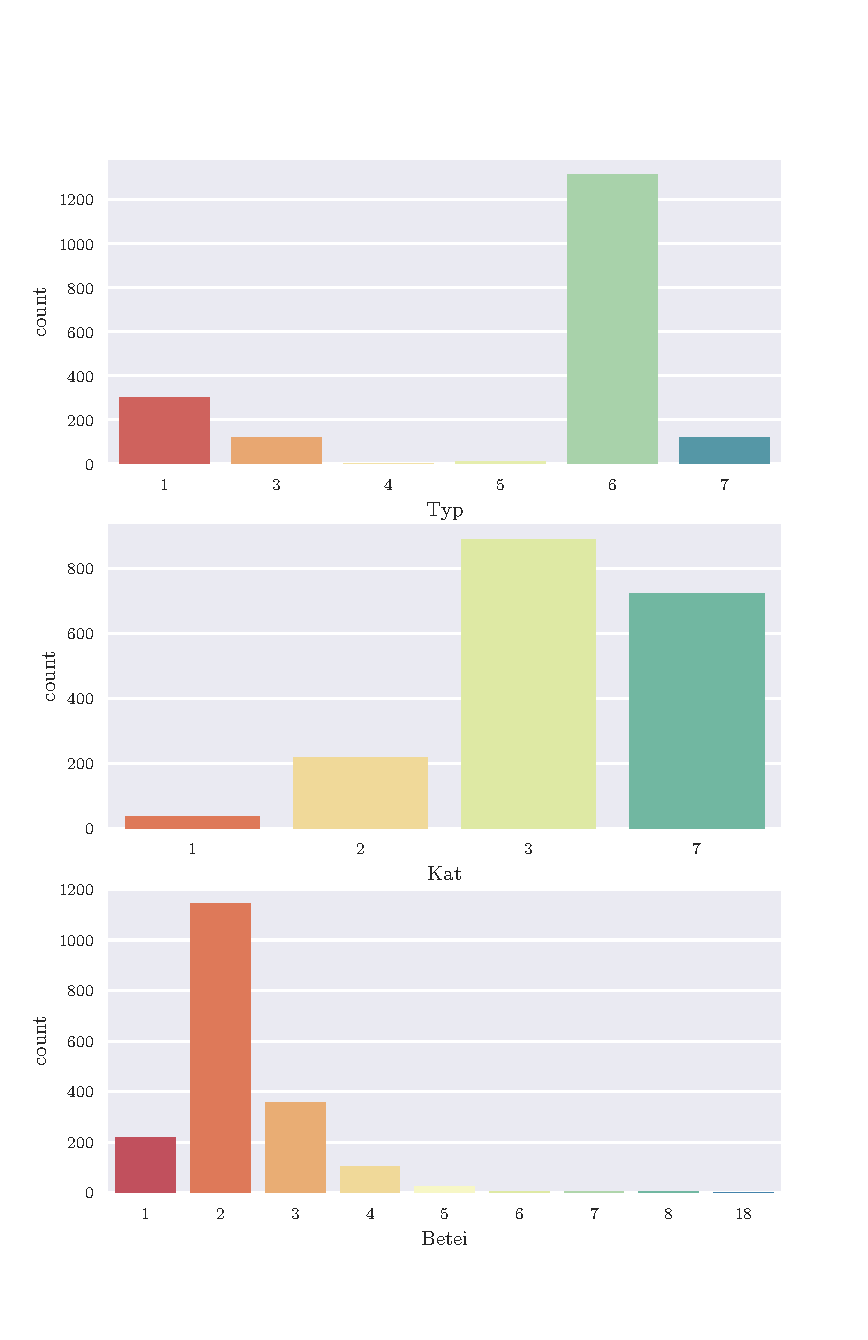
\includegraphics[scale=0.7]{../CorrAnalysis/data/BAYSIS/02_matched/plots/baysis_matched_count_multiple01}
    % 	\caption{Distribution of the accident category '', ...}
    % 	\label{img:appendix_baysis_matched_01}
    % \end{figure}
    
    % \begin{figure}[h]
    % 	\centering
    % 	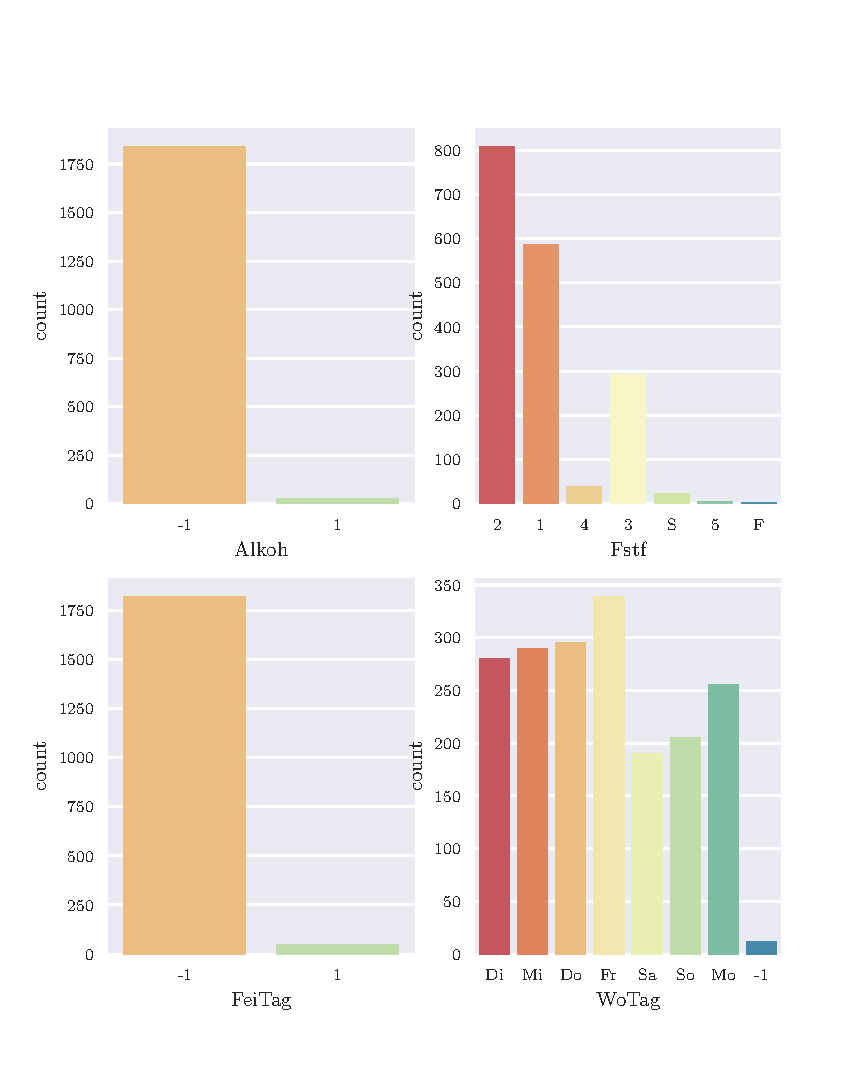
\includegraphics[scale=0.7]{../CorrAnalysis/data/BAYSIS/02_matched/plots/baysis_matched_count_multiple02}
    % 	\caption{Distribution of the accident category '', ..}
    % 	\label{img:appendix_baysis_matched_02}
    % \end{figure}
    
    % \begin{figure}[h]
    % 	\centering
    % 	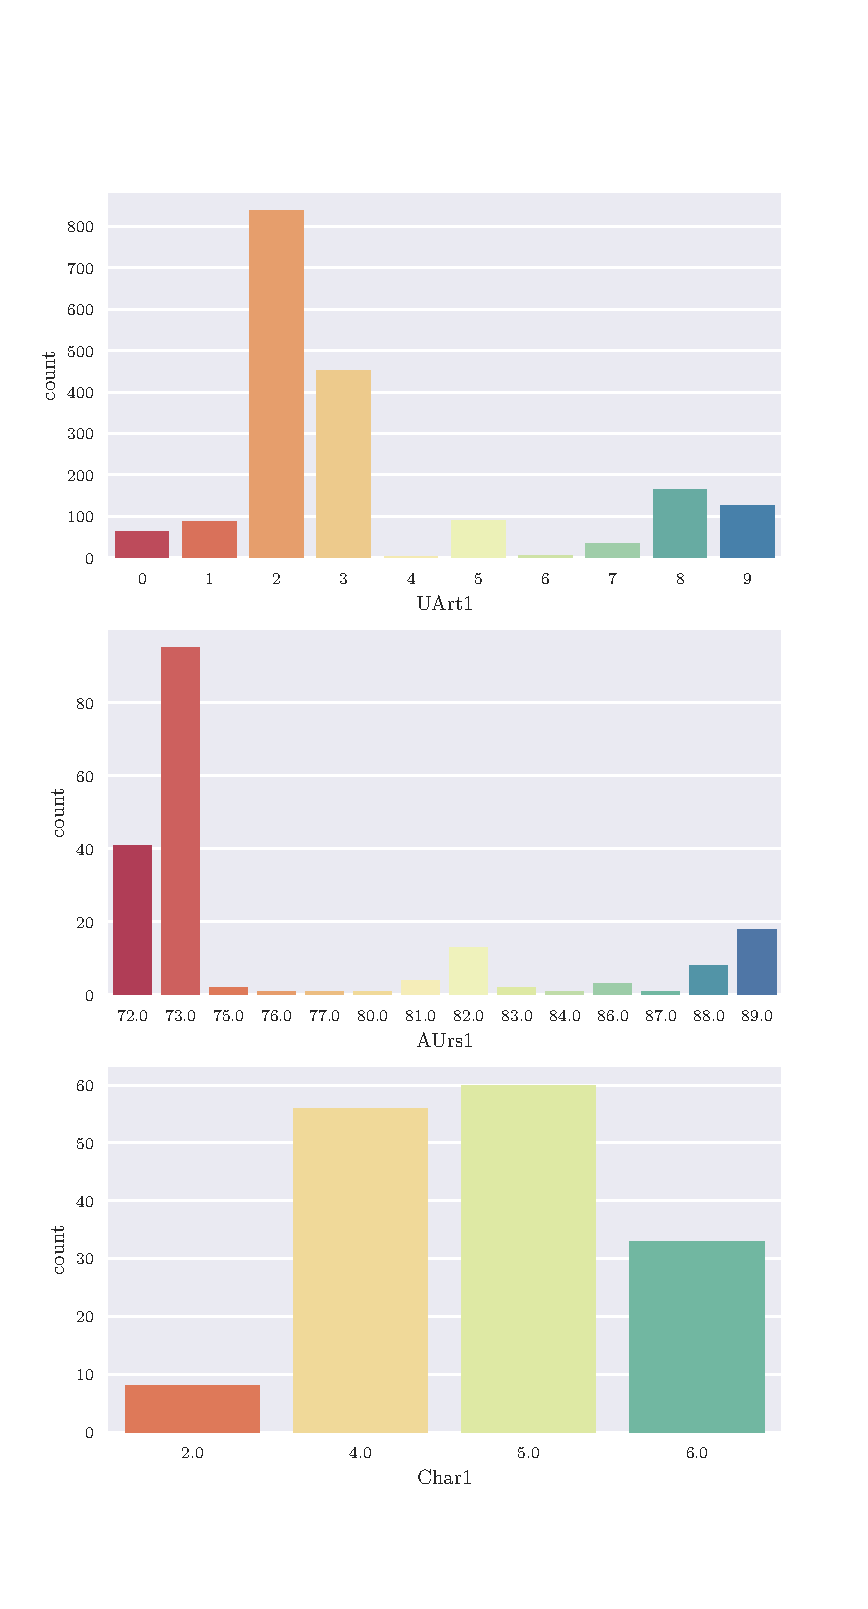
\includegraphics[scale=0.7]{../CorrAnalysis/data/BAYSIS/02_matched/plots/baysis_matched_count_multiple03}
    % 	\caption{Distribution of the accident category '', ..}
    % 	\label{img:appendix_baysis_matched_03}
    % \end{figure}
    
    % \begin{figure}[h]
    % 	\centering
    % 	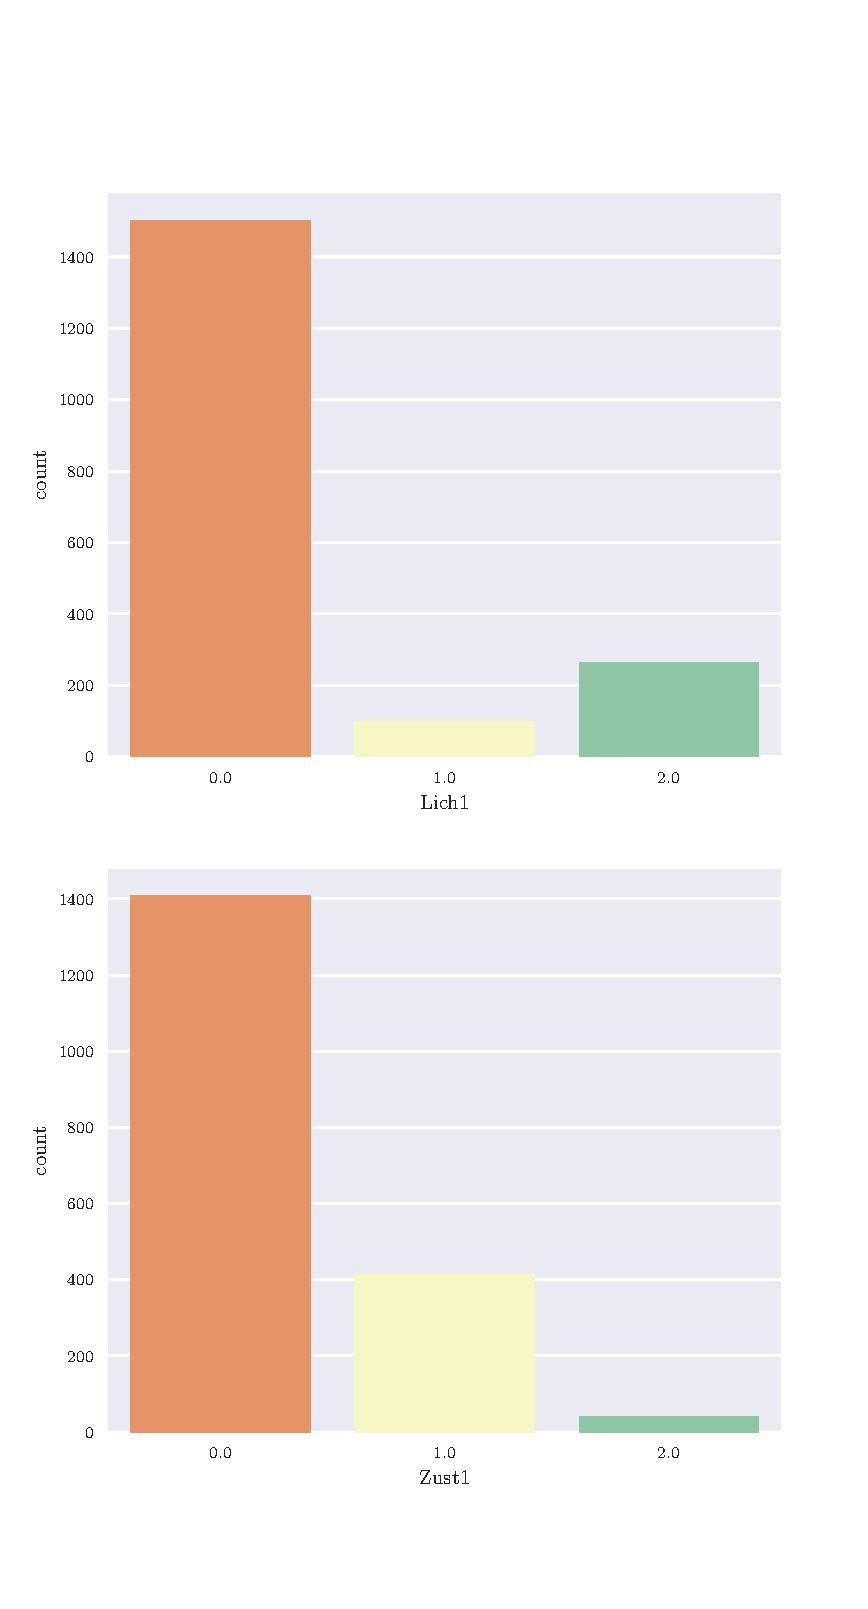
\includegraphics[scale=0.7]{../CorrAnalysis/data/BAYSIS/02_matched/plots/baysis_matched_count_multiple04}
    % 	\caption{Distribution of the accident category '', ...}
    % 	\label{img:appendix_baysis_matched_04}
    % \end{figure}
    % ------- BAYSIS Matched - Tables --------
    \newgeometry{left=1cm,right=1cm,bottom=2cm}
    \begin{sidewaystable}
    	\tiny
    	\setlength{\tabcolsep}{2pt}
    	\centering
    	\begin{tabular}{lrrrrrrrrrrrrrrrrrrrrrrrrrrrrrr}
\toprule
{} &  TempExMax &  SpatExMax &  TempDist &  SpatDist &  Coverage &  TimeLossCar &  TimeLossHGV &  Strasse &  Kat &  Typ &  Betei &  UArt1 &  UArt2 &  AUrs1 &  AUrs2 &  AufHi &  Alkoh &  Char1 &  Char2 &  Bes1 &  Bes2 &  Lich1 &  Lich2 &  Zust1 &  Zust2 &  Fstf &  StrklVu &  WoTag &  FeiTag &  Month \\
\midrule
TempExMax   &       1.00 &       0.46 &     -0.29 &     -0.08 &     -0.28 &         0.04 &        -0.01 &     0.27 & 0.14 & 0.08 &   0.10 &   0.13 &   0.09 &   0.14 &   0.07 &   0.15 &  -0.01 &   0.05 &   0.05 &  0.11 &  0.03 &   0.05 &   0.05 &   0.13 &   0.00 & -0.01 &     0.03 &   0.10 &   -0.00 &   0.13 \\
SpatExMax   &       0.46 &       1.00 &     -0.18 &     -0.08 &     -0.39 &        -0.03 &         0.02 &     0.25 & 0.04 & 0.07 &   0.08 &   0.11 &   0.08 &   0.09 &   0.03 &   0.10 &  -0.03 &   0.05 &   0.03 &  0.04 &  0.02 &   0.06 &   0.06 &   0.07 &   0.01 &  0.02 &     0.01 &   0.13 &    0.02 &   0.12 \\
TempDist    &      -0.29 &      -0.18 &      1.00 &      0.03 &      0.31 &        -0.04 &         0.00 &     0.19 & 0.20 & 0.28 &  -0.05 &   0.31 &   0.13 &   0.23 &   0.14 &   0.27 &   0.01 &   0.12 &   0.10 &  0.12 &  0.06 &   0.19 &   0.19 &   0.17 &   0.04 &  0.05 &     0.01 &   0.13 &    0.01 &   0.11 \\
SpatDist    &      -0.08 &      -0.08 &      0.03 &      1.00 &      0.05 &        -0.00 &         0.03 &     0.09 & 0.06 & 0.03 &  -0.02 &   0.07 &   0.05 &   0.10 &   0.02 &   0.06 &  -0.02 &   0.05 &   0.00 &  0.03 &  0.04 &   0.08 &   0.03 &   0.06 &   0.01 &  0.02 &     0.07 &   0.07 &    0.02 &   0.07 \\
Coverage    &      -0.28 &      -0.39 &      0.31 &      0.05 &      1.00 &         0.04 &        -0.01 &     0.30 & 0.11 & 0.22 &  -0.03 &   0.25 &   0.11 &   0.20 &   0.10 &   0.22 &   0.07 &   0.10 &   0.08 &  0.09 &  0.02 &   0.15 &   0.14 &   0.17 &   0.02 &  0.02 &     0.02 &   0.16 &    0.01 &   0.14 \\
TimeLossCar &       0.04 &      -0.03 &     -0.04 &     -0.00 &      0.04 &         1.00 &        -0.02 &     0.09 & 0.05 & 0.07 &   0.01 &   0.06 &   0.06 &   0.08 &   0.06 &   0.06 &  -0.04 &   0.04 &   0.02 &  0.01 &  0.01 &   0.03 &   0.01 &   0.05 &   0.03 & -0.03 &     0.03 &   0.08 &    0.03 &   0.08 \\
TimeLossHGV &      -0.01 &       0.02 &      0.00 &      0.03 &     -0.01 &        -0.02 &         1.00 &     0.09 & 0.05 & 0.05 &  -0.00 &   0.08 &   0.05 &   0.11 &   0.05 &   0.07 &   0.04 &   0.06 &   0.02 &  0.03 &  0.01 &   0.06 &   0.04 &   0.02 &   0.01 & -0.00 &     0.02 &   0.05 &   -0.05 &   0.06 \\
Strasse     &       0.27 &       0.25 &      0.19 &      0.09 &      0.30 &         0.09 &         0.09 &     1.00 & 0.13 & 0.12 &   0.09 &   0.10 &   0.10 &   0.11 &   0.06 &   0.10 &   0.06 &   0.16 &   0.10 &  0.17 &  0.17 &   0.12 &   0.12 &   0.14 &   0.11 &  0.16 &     0.09 &   0.12 &    0.09 &   0.11 \\
Kat         &       0.14 &       0.04 &      0.20 &      0.06 &      0.11 &         0.05 &         0.05 &     0.13 & 1.00 & 0.20 &   0.20 &   0.34 &   0.12 &   0.11 &   0.05 &   0.17 &   0.05 &   0.08 &   0.06 &  0.14 &  0.04 &   0.06 &   0.06 &   0.06 &   0.06 &  0.09 &     0.03 &   0.08 &    0.06 &   0.09 \\
Typ         &       0.08 &       0.07 &      0.28 &      0.03 &      0.22 &         0.07 &         0.05 &     0.12 & 0.20 & 1.00 &   0.31 &   0.61 &   0.09 &   0.27 &   0.08 &   0.26 &   0.10 &   0.14 &   0.20 &  0.13 &  0.06 &   0.08 &   0.09 &   0.21 &   0.15 &  0.12 &     0.05 &   0.10 &    0.06 &   0.09 \\
Betei       &       0.10 &       0.08 &     -0.05 &     -0.02 &     -0.03 &         0.01 &        -0.00 &     0.09 & 0.20 & 0.31 &   1.00 &   0.30 &   0.08 &   0.18 &   0.30 &   0.20 &   0.04 &   0.08 &   0.13 &  0.08 &  0.03 &   0.08 &   0.07 &   0.14 &   0.28 &  0.09 &     0.04 &   0.09 &    0.05 &   0.09 \\
UArt1       &       0.13 &       0.11 &      0.31 &      0.07 &      0.25 &         0.06 &         0.08 &     0.10 & 0.34 & 0.61 &   0.30 &   1.00 &   0.11 &   0.21 &   0.10 &   0.30 &   0.11 &   0.16 &   0.18 &  0.17 &  0.09 &   0.09 &   0.08 &   0.19 &   0.10 &  0.14 &     0.09 &   0.12 &    0.07 &   0.08 \\
UArt2       &       0.09 &       0.08 &      0.13 &      0.05 &      0.11 &         0.06 &         0.05 &     0.10 & 0.12 & 0.09 &   0.08 &   0.11 &   1.00 &   0.13 &   0.05 &   0.24 &   0.02 &   0.08 &   0.11 &  0.08 &  0.01 &   0.07 &   0.07 &   0.07 &   0.04 &  0.08 &     0.05 &   0.07 &    0.04 &   0.08 \\
AUrs1       &       0.14 &       0.09 &      0.23 &      0.10 &      0.20 &         0.08 &         0.11 &     0.11 & 0.11 & 0.27 &   0.18 &   0.21 &   0.13 &   1.00 &   0.35 &   0.16 &   0.03 &   0.11 &   0.17 &  0.29 &  0.71 &   0.09 &   0.09 &   0.48 &   0.52 &  0.06 &     0.01 &   0.11 &    0.05 &   0.14 \\
AUrs2       &       0.07 &       0.03 &      0.14 &      0.02 &      0.10 &         0.06 &         0.05 &     0.06 & 0.05 & 0.08 &   0.30 &   0.10 &   0.05 &   0.35 &   1.00 &   0.05 &   0.01 &   0.05 &   0.10 &  0.19 &  0.00 &   0.05 &   0.04 &   0.18 &   0.56 &  0.04 &     0.00 &   0.08 &    0.01 &   0.10 \\
AufHi       &       0.15 &       0.10 &      0.27 &      0.06 &      0.22 &         0.06 &         0.07 &     0.10 & 0.17 & 0.26 &   0.20 &   0.30 &   0.24 &   0.16 &   0.05 &   1.00 &   0.03 &   0.09 &   0.19 &  0.12 &  0.02 &   0.07 &   0.07 &   0.17 &   0.09 &  0.09 &     0.04 &   0.09 &    0.06 &   0.08 \\
Alkoh       &      -0.01 &      -0.03 &      0.01 &     -0.02 &      0.07 &        -0.04 &         0.04 &     0.06 & 0.05 & 0.10 &   0.04 &   0.11 &   0.02 &   0.03 &   0.01 &   0.03 &   1.00 &   0.06 &   0.00 &  0.01 &  0.07 &   0.12 &   0.11 &   0.02 &   0.01 &  0.06 &     0.01 &   0.04 &    0.00 &   0.07 \\
Char1       &       0.05 &       0.05 &      0.12 &      0.05 &      0.10 &         0.04 &         0.06 &     0.16 & 0.08 & 0.14 &   0.08 &   0.16 &   0.08 &   0.11 &   0.05 &   0.09 &   0.06 &   1.00 &   0.59 &  0.07 &  0.01 &   0.06 &   0.07 &   0.08 &   0.05 &  0.06 &     0.01 &   0.06 &    0.03 &   0.08 \\
Char2       &       0.05 &       0.03 &      0.10 &      0.00 &      0.08 &         0.02 &         0.02 &     0.10 & 0.06 & 0.20 &   0.13 &   0.18 &   0.11 &   0.17 &   0.10 &   0.19 &   0.00 &   0.59 &   1.00 &  0.06 &  0.05 &   0.07 &   0.07 &   0.13 &   0.00 &  0.11 &     0.01 &   0.08 &    0.03 &   0.07 \\
Bes1        &       0.11 &       0.04 &      0.12 &      0.03 &      0.09 &         0.01 &         0.03 &     0.17 & 0.14 & 0.13 &   0.08 &   0.17 &   0.08 &   0.29 &   0.19 &   0.12 &   0.01 &   0.07 &   0.06 &  1.00 &  0.53 &   0.05 &   0.05 &   0.07 &   0.05 &  0.10 &     0.02 &   0.07 &    0.02 &   0.14 \\
Bes2        &       0.03 &       0.02 &      0.06 &      0.04 &      0.02 &         0.01 &         0.01 &     0.17 & 0.04 & 0.06 &   0.03 &   0.09 &   0.01 &   0.71 &   0.00 &   0.02 &   0.07 &   0.01 &   0.05 &  0.53 &  1.00 &   0.02 &   0.02 &   0.02 &   0.08 &  0.05 &     0.00 &   0.05 &    0.05 &   0.08 \\
Lich1       &       0.05 &       0.06 &      0.19 &      0.08 &      0.15 &         0.03 &         0.06 &     0.12 & 0.06 & 0.08 &   0.08 &   0.09 &   0.07 &   0.09 &   0.05 &   0.07 &   0.12 &   0.06 &   0.07 &  0.05 &  0.02 &   1.00 &   0.71 &   0.43 &   0.03 &  0.06 &     0.04 &   0.06 &    0.02 &   0.21 \\
Lich2       &       0.05 &       0.06 &      0.19 &      0.03 &      0.14 &         0.01 &         0.04 &     0.12 & 0.06 & 0.09 &   0.07 &   0.08 &   0.07 &   0.09 &   0.04 &   0.07 &   0.11 &   0.07 &   0.07 &  0.05 &  0.02 &   0.71 &   1.00 &   0.16 &   0.02 &  0.05 &     0.04 &   0.06 &    0.03 &   0.25 \\
Zust1       &       0.13 &       0.07 &      0.17 &      0.06 &      0.17 &         0.05 &         0.02 &     0.14 & 0.06 & 0.21 &   0.14 &   0.19 &   0.07 &   0.48 &   0.18 &   0.17 &   0.02 &   0.08 &   0.13 &  0.07 &  0.02 &   0.43 &   0.16 &   1.00 &   0.19 &  0.06 &     0.03 &   0.08 &    0.04 &   0.28 \\
Zust2       &       0.00 &       0.01 &      0.04 &      0.01 &      0.02 &         0.03 &         0.01 &     0.11 & 0.06 & 0.15 &   0.28 &   0.10 &   0.04 &   0.52 &   0.56 &   0.09 &   0.01 &   0.05 &   0.00 &  0.05 &  0.08 &   0.03 &   0.02 &   0.19 &   1.00 &  0.04 &     0.01 &   0.09 &    0.00 &   0.21 \\
Fstf        &      -0.01 &       0.02 &      0.05 &      0.02 &      0.02 &        -0.03 &        -0.00 &     0.16 & 0.09 & 0.12 &   0.09 &   0.14 &   0.08 &   0.06 &   0.04 &   0.09 &   0.06 &   0.06 &   0.11 &  0.10 &  0.05 &   0.06 &   0.05 &   0.06 &   0.04 &  1.00 &     0.07 &   0.07 &    0.04 &   0.09 \\
StrklVu     &       0.03 &       0.01 &      0.01 &      0.07 &      0.02 &         0.03 &         0.02 &     0.09 & 0.03 & 0.05 &   0.04 &   0.09 &   0.05 &   0.01 &   0.00 &   0.04 &   0.01 &   0.01 &   0.01 &  0.02 &  0.00 &   0.04 &   0.04 &   0.03 &   0.01 &  0.07 &     1.00 &   0.05 &    0.01 &   0.09 \\
WoTag       &       0.10 &       0.13 &      0.13 &      0.07 &      0.16 &         0.08 &         0.05 &     0.12 & 0.08 & 0.10 &   0.09 &   0.12 &   0.07 &   0.11 &   0.08 &   0.09 &   0.04 &   0.06 &   0.08 &  0.07 &  0.05 &   0.06 &   0.06 &   0.08 &   0.09 &  0.07 &     0.05 &   1.00 &    0.16 &   0.09 \\
FeiTag      &      -0.00 &       0.02 &      0.01 &      0.02 &      0.01 &         0.03 &        -0.05 &     0.09 & 0.06 & 0.06 &   0.05 &   0.07 &   0.04 &   0.05 &   0.01 &   0.06 &   0.00 &   0.03 &   0.03 &  0.02 &  0.05 &   0.02 &   0.03 &   0.04 &   0.00 &  0.04 &     0.01 &   0.16 &    1.00 &   0.17 \\
Month       &       0.13 &       0.12 &      0.11 &      0.07 &      0.14 &         0.08 &         0.06 &     0.11 & 0.09 & 0.09 &   0.09 &   0.08 &   0.08 &   0.14 &   0.10 &   0.08 &   0.07 &   0.08 &   0.07 &  0.14 &  0.08 &   0.21 &   0.25 &   0.28 &   0.21 &  0.09 &     0.09 &   0.09 &    0.17 &   1.00 \\
\bottomrule
\end{tabular}

    	\caption{Correlation matrix for BAYSIS matched data, with Cramer's $V$}
    	\label{table:appendix_correlation_matrix_matched_cramers}
    \end{sidewaystable}
    
    \newgeometry{left=1cm,right=1cm,bottom=2cm}
    \begin{sidewaystable}
    	\tiny
    	\setlength{\tabcolsep}{2pt}
    	\centering
    	\begin{tabular}{lrrrrrrrrrrrrrrrrrrrrrrrrrrrrrrr}
\toprule
{} &  TempExMax &  SpatExMax &  TempDist &  SpatDist &  Coverage &  TimeLossCar &  TimeLossHGV &  Strasse &  Kat &  Typ &  Betei &  UArt1 &  UArt2 &  AUrs1 &  AUrs2 &  AufHi &  Alkoh &  Char1 &  Char2 &  Bes1 &  Bes2 &  Lich1 &  Lich2 &  Zust1 &  Zust2 &  Fstf &  StrklVu &  WoTagNr &  WoTag &  FeiTag &  Month \\
\midrule
TempExMax   &       1.00 &       0.46 &     -0.29 &     -0.08 &     -0.28 &         0.04 &        -0.01 &     0.27 & 0.14 & 0.08 &   0.10 &   0.13 &   0.09 &   0.14 &   0.07 &   0.15 &  -0.01 &   0.05 &   0.05 &  0.11 &  0.03 &   0.05 &   0.05 &   0.13 &   0.00 & -0.01 &     0.03 &     0.01 &   0.10 &   -0.00 &   0.13 \\
SpatExMax   &       0.46 &       1.00 &     -0.18 &     -0.08 &     -0.39 &        -0.03 &         0.02 &     0.25 & 0.04 & 0.07 &   0.08 &   0.11 &   0.08 &   0.09 &   0.03 &   0.10 &  -0.03 &   0.05 &   0.03 &  0.04 &  0.02 &   0.06 &   0.06 &   0.07 &   0.01 &  0.02 &     0.01 &     0.08 &   0.13 &    0.02 &   0.12 \\
TempDist    &      -0.29 &      -0.18 &      1.00 &      0.03 &      0.31 &        -0.04 &         0.00 &     0.19 & 0.20 & 0.28 &  -0.05 &   0.31 &   0.13 &   0.23 &   0.14 &   0.27 &   0.01 &   0.12 &   0.10 &  0.12 &  0.06 &   0.19 &   0.19 &   0.17 &   0.04 &  0.05 &     0.01 &    -0.05 &   0.13 &    0.01 &   0.11 \\
SpatDist    &      -0.08 &      -0.08 &      0.03 &      1.00 &      0.05 &        -0.00 &         0.03 &     0.09 & 0.06 & 0.03 &  -0.02 &   0.07 &   0.05 &   0.10 &   0.02 &   0.06 &  -0.02 &   0.05 &   0.00 &  0.03 &  0.04 &   0.08 &   0.03 &   0.06 &   0.01 &  0.02 &     0.07 &    -0.03 &   0.07 &    0.02 &   0.07 \\
Coverage    &      -0.28 &      -0.39 &      0.31 &      0.05 &      1.00 &         0.04 &        -0.01 &     0.30 & 0.11 & 0.22 &  -0.03 &   0.25 &   0.11 &   0.20 &   0.10 &   0.22 &   0.07 &   0.10 &   0.08 &  0.09 &  0.02 &   0.15 &   0.14 &   0.17 &   0.02 &  0.02 &     0.02 &    -0.07 &   0.16 &    0.01 &   0.14 \\
TimeLossCar &       0.04 &      -0.03 &     -0.04 &     -0.00 &      0.04 &         1.00 &        -0.02 &     0.09 & 0.05 & 0.07 &   0.01 &   0.06 &   0.06 &   0.08 &   0.06 &   0.06 &  -0.04 &   0.04 &   0.02 &  0.01 &  0.01 &   0.03 &   0.01 &   0.05 &   0.03 & -0.03 &     0.03 &     0.01 &   0.08 &    0.03 &   0.08 \\
TimeLossHGV &      -0.01 &       0.02 &      0.00 &      0.03 &     -0.01 &        -0.02 &         1.00 &     0.09 & 0.05 & 0.05 &  -0.00 &   0.08 &   0.05 &   0.11 &   0.05 &   0.07 &   0.04 &   0.06 &   0.02 &  0.03 &  0.01 &   0.06 &   0.04 &   0.02 &   0.01 & -0.00 &     0.02 &     0.03 &   0.05 &   -0.05 &   0.06 \\
Strasse     &       0.27 &       0.25 &      0.19 &      0.09 &      0.30 &         0.09 &         0.09 &     1.00 & 0.01 & 0.02 &   0.02 &   0.02 &   0.02 &   0.02 &   0.00 &   0.02 &   0.00 &   0.02 &   0.00 &  0.01 &  0.00 &   0.01 &   0.01 &   0.01 &   0.00 &  0.04 &     0.00 &     0.12 &   0.02 &    0.00 &   0.03 \\
Kat         &       0.14 &       0.04 &      0.20 &      0.06 &      0.11 &         0.05 &         0.05 &     0.02 & 1.00 & 0.05 &   0.06 &   0.15 &   0.02 &   0.01 &   0.00 &   0.02 &   0.00 &   0.01 &   0.00 &  0.02 &  0.00 &   0.00 &   0.00 &   0.01 &   0.00 &  0.01 &     0.00 &     0.04 &   0.01 &    0.00 &   0.01 \\
Typ         &       0.08 &       0.07 &      0.28 &      0.03 &      0.22 &         0.07 &         0.05 &     0.04 & 0.06 & 1.00 &   0.22 &   0.39 &   0.02 &   0.12 &   0.01 &   0.16 &   0.00 &   0.03 &   0.02 &  0.01 &  0.00 &   0.01 &   0.01 &   0.06 &   0.01 &  0.03 &     0.00 &     0.06 &   0.02 &    0.00 &   0.02 \\
Betei       &       0.10 &       0.08 &     -0.05 &     -0.02 &     -0.03 &         0.01 &        -0.00 &     0.03 & 0.06 & 0.18 &   1.00 &   0.25 &   0.02 &   0.06 &   0.01 &   0.12 &   0.00 &   0.01 &   0.01 &  0.01 &  0.00 &   0.01 &   0.00 &   0.02 &   0.01 &  0.02 &     0.00 &     0.02 &   0.02 &    0.00 &   0.03 \\
UArt1       &       0.13 &       0.11 &      0.31 &      0.07 &      0.25 &         0.06 &         0.08 &     0.03 & 0.10 & 0.23 &   0.18 &   1.00 &   0.04 &   0.06 &   0.01 &   0.20 &   0.00 &   0.02 &   0.01 &  0.02 &  0.00 &   0.01 &   0.00 &   0.03 &   0.00 &  0.04 &     0.00 &     0.07 &   0.03 &    0.00 &   0.02 \\
UArt2       &       0.09 &       0.08 &      0.13 &      0.05 &      0.11 &         0.06 &         0.05 &     0.05 & 0.03 & 0.03 &   0.03 &   0.09 &   1.00 &   0.03 &   0.01 &   0.33 &   0.00 &   0.01 &   0.01 &  0.02 &  0.00 &   0.01 &   0.01 &   0.01 &   0.00 &  0.03 &     0.00 &     0.09 &   0.02 &    0.00 &   0.04 \\
AUrs1       &       0.14 &       0.09 &      0.23 &      0.10 &      0.20 &         0.08 &         0.11 &     0.09 & 0.03 & 0.22 &   0.14 &   0.20 &   0.04 &   1.00 &   0.06 &   0.15 &   0.00 &   0.03 &   0.02 &  0.03 &  0.01 &   0.02 &   0.02 &   0.32 &   0.06 &  0.02 &     0.00 &     0.10 &   0.06 &    0.00 &   0.15 \\
AUrs2       &       0.07 &       0.03 &      0.14 &      0.02 &      0.10 &         0.06 &         0.05 &     0.15 & 0.05 & 0.19 &   0.24 &   0.23 &   0.07 &   0.50 &   1.00 &   0.10 &   0.00 &   0.04 &   0.02 &  0.06 &  0.00 &   0.05 &   0.03 &   0.25 &   0.27 &  0.08 &     0.00 &     0.09 &   0.21 &    0.00 &   0.27 \\
AufHi       &       0.15 &       0.10 &      0.27 &      0.06 &      0.22 &         0.06 &         0.07 &     0.04 & 0.03 & 0.20 &   0.19 &   0.43 &   0.27 &   0.10 &   0.01 &   1.00 &   0.00 &   0.02 &   0.02 &  0.02 &  0.00 &   0.01 &   0.01 &   0.05 &   0.00 &  0.03 &     0.00 &     0.08 &   0.03 &    0.00 &   0.03 \\
Alkoh       &      -0.01 &      -0.03 &      0.01 &     -0.02 &      0.07 &        -0.04 &         0.04 &     0.03 & 0.01 & 0.03 &   0.01 &   0.06 &   0.01 &   0.01 &   0.00 &   0.01 &   1.00 &   0.02 &   0.00 &  0.00 &  0.00 &   0.08 &   0.07 &   0.00 &   0.00 &  0.03 &     0.00 &     0.01 &   0.02 &    0.00 &   0.03 \\
Char1       &       0.05 &       0.05 &      0.12 &      0.05 &      0.10 &         0.04 &         0.06 &     0.08 & 0.02 & 0.06 &   0.03 &   0.07 &   0.02 &   0.03 &   0.01 &   0.03 &   0.00 &   1.00 &   0.17 &  0.01 &  0.00 &   0.01 &   0.01 &   0.02 &   0.00 &  0.02 &     0.00 &     0.06 &   0.02 &    0.00 &   0.03 \\
Char2       &       0.05 &       0.03 &      0.10 &      0.00 &      0.08 &         0.02 &         0.02 &     0.05 & 0.01 & 0.13 &   0.06 &   0.11 &   0.03 &   0.08 &   0.01 &   0.13 &   0.00 &   0.62 &   1.00 &  0.01 &  0.00 &   0.02 &   0.02 &   0.06 &   0.00 &  0.06 &     0.00 &     0.06 &   0.03 &    0.01 &   0.02 \\
Bes1        &       0.11 &       0.04 &      0.12 &      0.03 &      0.09 &         0.01 &         0.03 &     0.05 & 0.04 & 0.02 &   0.02 &   0.06 &   0.02 &   0.04 &   0.01 &   0.04 &   0.00 &   0.00 &   0.00 &  1.00 &  0.01 &   0.00 &   0.01 &   0.01 &   0.00 &  0.03 &     0.00 &     0.04 &   0.01 &    0.00 &   0.04 \\
Bes2        &       0.03 &       0.02 &      0.06 &      0.04 &      0.02 &         0.01 &         0.01 &     0.36 & 0.13 & 0.11 &   0.05 &   0.22 &   0.02 &   0.46 &   0.00 &   0.04 &   0.00 &   0.01 &   0.00 &  0.73 &  1.00 &   0.03 &   0.03 &   0.04 &   0.00 &  0.15 &     0.00 &     0.02 &   0.14 &    0.00 &   0.23 \\
Lich1       &       0.05 &       0.06 &      0.19 &      0.08 &      0.15 &         0.03 &         0.06 &     0.03 & 0.01 & 0.01 &   0.01 &   0.01 &   0.01 &   0.02 &   0.00 &   0.01 &   0.01 &   0.01 &   0.00 &  0.00 &  0.00 &   1.00 &   0.80 &   0.05 &   0.00 &  0.01 &     0.00 &     0.04 &   0.01 &    0.00 &   0.10 \\
Lich2       &       0.05 &       0.06 &      0.19 &      0.03 &      0.14 &         0.01 &         0.04 &     0.03 & 0.01 & 0.01 &   0.01 &   0.01 &   0.01 &   0.02 &   0.00 &   0.01 &   0.01 &   0.01 &   0.00 &  0.00 &  0.00 &   0.93 &   1.00 &   0.04 &   0.00 &  0.00 &     0.00 &     0.03 &   0.01 &    0.00 &   0.11 \\
Zust1       &       0.13 &       0.07 &      0.17 &      0.06 &      0.17 &         0.05 &         0.02 &     0.03 & 0.01 & 0.08 &   0.04 &   0.07 &   0.01 &   0.25 &   0.02 &   0.06 &   0.00 &   0.01 &   0.01 &  0.01 &  0.00 &   0.05 &   0.03 &   1.00 &   0.02 &  0.01 &     0.00 &     0.05 &   0.02 &    0.00 &   0.12 \\
Zust2       &       0.00 &       0.01 &      0.04 &      0.01 &      0.02 &         0.03 &         0.01 &     0.10 & 0.03 & 0.15 &   0.17 &   0.07 &   0.01 &   0.50 &   0.29 &   0.06 &   0.00 &   0.02 &   0.00 &  0.04 &  0.00 &   0.00 &   0.00 &   0.27 &   1.00 &  0.02 &     0.00 &     0.02 &   0.07 &    0.00 &   0.25 \\
Fstf        &      -0.01 &       0.02 &      0.05 &      0.02 &      0.02 &        -0.03 &        -0.00 &     0.07 & 0.01 & 0.02 &   0.02 &   0.04 &   0.01 &   0.01 &   0.00 &   0.02 &   0.00 &   0.01 &   0.00 &  0.01 &  0.00 &   0.00 &   0.00 &   0.00 &   0.00 &  1.00 &     0.00 &    -0.02 &   0.01 &    0.00 &   0.02 \\
StrklVu     &       0.03 &       0.01 &      0.01 &      0.07 &      0.02 &         0.03 &         0.02 &     0.16 & 0.04 & 0.11 &   0.08 &   0.23 &   0.06 &   0.02 &   0.00 &   0.07 &   0.00 &   0.01 &   0.00 &  0.03 &  0.00 &   0.08 &   0.07 &   0.04 &   0.00 &  0.14 &     1.00 &     0.03 &   0.14 &    0.00 &   0.23 \\
WoTagNr     &       0.01 &       0.08 &     -0.05 &     -0.03 &     -0.07 &         0.01 &         0.03 &     0.12 & 0.04 & 0.06 &   0.02 &   0.07 &   0.09 &   0.10 &   0.09 &   0.08 &   0.01 &   0.06 &   0.06 &  0.04 &  0.02 &   0.04 &   0.03 &   0.05 &   0.02 & -0.02 &     0.03 &     1.00 &   1.00 &    0.00 &   0.11 \\
WoTag       &       0.10 &       0.13 &      0.13 &      0.07 &      0.16 &         0.08 &         0.05 &     0.02 & 0.00 & 0.01 &   0.01 &   0.02 &   0.01 &   0.02 &   0.01 &   0.01 &   0.00 &   0.00 &   0.00 &  0.00 &  0.00 &   0.00 &   0.00 &   0.01 &   0.00 &  0.01 &     0.00 &     1.00 &   1.00 &    0.01 &   0.01 \\
FeiTag      &      -0.00 &       0.02 &      0.01 &      0.02 &      0.01 &         0.03 &        -0.05 &     0.04 & 0.02 & 0.02 &   0.01 &   0.03 &   0.01 &   0.01 &   0.00 &   0.01 &   0.00 &   0.01 &   0.01 &  0.00 &  0.00 &   0.00 &   0.00 &   0.01 &   0.00 &  0.01 &     0.00 &     0.00 &   0.10 &    1.00 &   0.13 \\
Month       &       0.13 &       0.12 &      0.11 &      0.07 &      0.14 &         0.08 &         0.06 &     0.02 & 0.00 & 0.01 &   0.01 &   0.01 &   0.01 &   0.03 &   0.01 &   0.01 &   0.00 &   0.01 &   0.00 &  0.01 &  0.00 &   0.03 &   0.02 &   0.03 &   0.01 &  0.01 &     0.00 &     0.11 &   0.01 &    0.01 &   1.00 \\
\bottomrule
\end{tabular}

    	\caption{Correlation matrix for BAYSIS matched data, with Theil's $U$}
    	\label{table:appendix_correlation_matrix_matched_theils}
    \end{sidewaystable}
    
    \newgeometry{left=1cm,right=1cm,bottom=2cm}
    \begin{sidewaystable}
    	\fontsize{3}{5}\selectfont
    	\setlength{\tabcolsep}{2pt}
    	\centering
    	\begin{tabular}{lrrrrrrrrrrrrrrrrrrrrrrrrrrrrrr}
\toprule
{} &  TempExMax &  SpatExMax &  TempDist &  SpatDist &  Coverage &  TimeLossCar &  TimeLossHGV &  Strasse &     Kat &     Typ &   Betei &   UArt1 &   UArt2 &   AUrs1 &   AUrs2 &   AufHi &   Alkoh &   Char1 &   Char2 &    Bes1 &    Bes2 &   Lich1 &   Lich2 &   Zust1 &   Zust2 &    Fstf &  StrklVu &   WoTag &  FeiTag &   Month \\
\midrule
TempExMax   &        NaN &     0.0000 &    0.0000 &    0.0004 &    0.0000 &       0.0663 &       0.8156 &   0.0000 &  0.0000 &  0.0000 &  0.0000 &  0.0000 &  0.0000 &  0.0000 &  0.0000 &  0.0000 &  0.6611 &  0.0000 &  0.0000 &  0.0000 &  0.0000 &  0.0000 &  0.0000 &  0.0000 &  0.0000 &  0.6820 &   0.0000 &  0.0000 &  0.9263 &  0.0000 \\
SpatExMax   &     0.0000 &        NaN &    0.0000 &    0.0008 &    0.0000 &       0.1348 &       0.4514 &   0.0000 &  0.0000 &  0.0000 &  0.0000 &  0.0000 &  0.0000 &  0.0000 &  0.0000 &  0.0000 &  0.1874 &  0.0000 &  0.0000 &  0.0000 &  0.0000 &  0.0000 &  0.0000 &  0.0000 &  0.0000 &  0.2676 &   0.0000 &  0.0000 &  0.2804 &  0.0000 \\
TempDist    &     0.0000 &     0.0000 &       NaN &    0.1760 &    0.0000 &       0.0906 &       0.9098 &   0.0000 &  0.0000 &  0.0000 &  0.0046 &  0.0265 &  0.0000 &  0.0000 &  0.0000 &  0.0000 &  0.5286 &  0.0000 &  0.0000 &  0.0000 &  0.0000 &  0.0000 &  0.0000 &  0.0000 &  0.0000 &  0.0123 &   0.0000 &  0.0177 &  0.4757 &  0.0000 \\
SpatDist    &     0.0004 &     0.0008 &    0.1760 &       NaN &    0.0464 &       0.8513 &       0.2108 &   0.0000 &  0.0000 &  0.0000 &  0.3364 &  0.0000 &  0.0000 &  0.0437 &  0.0000 &  0.0000 &  0.4761 &  0.0000 &  0.0000 &  0.0000 &  0.0000 &  0.0000 &  0.0000 &  0.0000 &  0.0000 &  0.2887 &   0.0000 &  0.0000 &  0.4151 &  0.0000 \\
Coverage    &     0.0000 &     0.0000 &    0.0000 &    0.0464 &       NaN &       0.0776 &       0.5694 &   0.0000 &  0.0000 &  0.0000 &  0.1270 &  0.0000 &  0.0000 &  0.0000 &  0.0000 &  0.0000 &  0.0015 &  0.0000 &  0.0000 &  0.0000 &  0.0000 &  0.0000 &  0.0000 &  0.0000 &  0.0000 &  0.2001 &   0.0000 &  0.0000 &  0.5254 &  0.0000 \\
TimeLossCar &     0.0663 &     0.1348 &    0.0906 &    0.8513 &    0.0776 &          NaN &       0.3760 &   0.0000 &  0.0000 &  0.0000 &  0.4375 &  0.0000 &  0.0000 &  0.0000 &  0.0000 &  0.0000 &  0.0856 &  0.0000 &  0.0000 &  0.0000 &  0.0000 &  0.0000 &  0.0000 &  0.0000 &  0.0000 &  0.1280 &   0.0000 &  0.0000 &  0.1686 &  0.0000 \\
TimeLossHGV &     0.8156 &     0.4514 &    0.9098 &    0.2108 &    0.5694 &       0.3760 &          NaN &   0.0000 &  0.0000 &  0.0000 &  0.9529 &  0.0000 &  0.0000 &  0.0000 &  0.0000 &  0.0000 &  0.0684 &  0.0000 &  0.0000 &  0.0000 &  0.0000 &  0.0000 &  0.0000 &  0.0000 &  0.0000 &  0.9851 &   0.0000 &  0.0000 &  0.0129 &  0.0000 \\
Strasse     &     0.0000 &     0.0000 &    0.0000 &    0.0000 &    0.0000 &       0.0000 &       0.0000 &      NaN &  0.0000 &  0.0000 &  0.3935 &  0.0551 &  0.0254 &  0.0000 &  1.0000 &  0.2356 &  0.9889 &  0.0000 &  0.3908 &  0.0000 &  0.0000 &  0.0035 &  0.0053 &  0.0000 &  0.1034 &  0.0000 &   0.5171 &  0.0001 &  0.4888 &  0.0000 \\
Kat         &     0.0000 &     0.0000 &    0.0000 &    0.0000 &    0.0000 &       0.0000 &       0.0000 &   0.0000 &     NaN &  0.0000 &  0.0000 &  0.0000 &  0.0000 &  0.0080 &  0.8138 &  0.0000 &  0.1756 &  0.0001 &  0.0891 &  0.0000 &  0.3412 &  0.0316 &  0.0294 &  0.0080 &  0.0840 &  0.0030 &   0.8763 &  0.0085 &  0.0629 &  0.1340 \\
Typ         &     0.0000 &     0.0000 &    0.0000 &    0.0000 &    0.0000 &       0.0000 &       0.0000 &   0.0000 &  0.0000 &     NaN &  0.0000 &  0.0000 &  0.0164 &  0.0000 &  0.0004 &  0.0000 &  0.0015 &  0.0000 &  0.0000 &  0.0000 &  0.2700 &  0.0077 &  0.0004 &  0.0000 &  0.0000 &  0.0000 &   0.3788 &  0.0000 &  0.2582 &  0.0166 \\
Betei       &     0.0000 &     0.0000 &    0.0046 &    0.3364 &    0.1270 &       0.4375 &       0.9529 &   0.3935 &  0.0000 &  0.0000 &     NaN &  0.0000 &  0.0729 &  0.0000 &  0.0000 &  0.0000 &  0.9489 &  0.0159 &  0.0001 &  0.0736 &  0.9933 &  0.0658 &  0.3250 &  0.0000 &  0.0000 &  0.0001 &   0.9855 &  0.0006 &  0.7143 &  0.0192 \\
UArt1       &     0.0000 &     0.0000 &    0.0265 &    0.0000 &    0.0000 &       0.0000 &       0.0000 &   0.0551 &  0.0000 &  0.0000 &  0.0000 &     NaN &  0.0000 &  0.0000 &  0.0000 &  0.0000 &  0.0082 &  0.0000 &  0.0000 &  0.0000 &  0.0893 &  0.0379 &  0.1579 &  0.0000 &  0.0448 &  0.0000 &   0.0226 &  0.0000 &  0.4417 &  0.2364 \\
UArt2       &     0.0000 &     0.0000 &    0.0000 &    0.0000 &    0.0000 &       0.0000 &       0.0000 &   0.0254 &  0.0000 &  0.0164 &  0.0729 &  0.0000 &     NaN &  0.0000 &  0.9988 &  0.0000 &  0.9996 &  0.0620 &  0.0091 &  0.1024 &  1.0000 &  0.3611 &  0.2868 &  0.4305 &  0.9676 &  0.0688 &   0.9174 &  0.3612 &  0.9686 &  0.2235 \\
AUrs1       &     0.0000 &     0.0000 &    0.0000 &    0.0437 &    0.0000 &       0.0000 &       0.0000 &   0.0000 &  0.0080 &  0.0000 &  0.0000 &  0.0000 &  0.0000 &     NaN &  0.0000 &  0.0000 &  1.0000 &  0.0078 &  0.0000 &  0.0000 &  0.0000 &  0.4621 &  0.2537 &  0.0000 &  0.0000 &  1.0000 &   1.0000 &  0.0002 &  0.9962 &  0.0000 \\
AUrs2       &     0.0000 &     0.0000 &    0.0000 &    0.0000 &    0.0000 &       0.0000 &       0.0000 &   1.0000 &  0.8138 &  0.0004 &  0.0000 &  0.0000 &  0.9988 &  0.0000 &     NaN &  0.9929 &  0.9998 &  0.7947 &  0.0029 &  0.0000 &  1.0000 &  0.7021 &  0.9268 &  0.0000 &  0.0000 &  0.9978 &   1.0000 &  0.0020 &  0.9988 &  0.0006 \\
AufHi       &     0.0000 &     0.0000 &    0.0000 &    0.0000 &    0.0000 &       0.0000 &       0.0000 &   0.2356 &  0.0000 &  0.0000 &  0.0000 &  0.0000 &  0.0000 &  0.0000 &  0.9929 &     NaN &  0.9964 &  0.0021 &  0.0000 &  0.0000 &  0.9995 &  0.3248 &  0.3736 &  0.0000 &  0.0488 &  0.0000 &   0.9906 &  0.0000 &  0.5950 &  0.2706 \\
Alkoh       &     0.6611 &     0.1874 &    0.5286 &    0.4761 &    0.0015 &       0.0856 &       0.0684 &   0.9889 &  0.1756 &  0.0015 &  0.9489 &  0.0082 &  0.9996 &  1.0000 &  0.9998 &  0.9964 &     NaN &  0.1594 &  0.9252 &  0.8996 &  0.0030 &  0.0000 &  0.0000 &  0.8794 &  0.6043 &  0.3950 &   0.9677 &  0.7630 &  0.8752 &  0.6965 \\
Char1       &     0.0000 &     0.0000 &    0.0000 &    0.0000 &    0.0000 &       0.0000 &       0.0000 &   0.0000 &  0.0001 &  0.0000 &  0.0159 &  0.0000 &  0.0620 &  0.0078 &  0.7947 &  0.0021 &  0.1594 &     NaN &  0.0000 &  0.0450 &  0.9955 &  0.0480 &  0.0194 &  0.0004 &  0.4275 &  0.4418 &   0.9999 &  0.4278 &  0.8417 &  0.4014 \\
Char2       &     0.0000 &     0.0000 &    0.0000 &    0.0000 &    0.0000 &       0.0000 &       0.0000 &   0.3908 &  0.0891 &  0.0000 &  0.0001 &  0.0000 &  0.0091 &  0.0000 &  0.0029 &  0.0000 &  0.9252 &  0.0000 &     NaN &  0.0373 &  0.0354 &  0.0228 &  0.0065 &  0.0000 &  0.9407 &  0.0011 &   0.9409 &  0.0382 &  0.1911 &  0.6015 \\
Bes1        &     0.0000 &     0.0000 &    0.0000 &    0.0000 &    0.0000 &       0.0000 &       0.0000 &   0.0000 &  0.0000 &  0.0000 &  0.0736 &  0.0000 &  0.1024 &  0.0000 &  0.0000 &  0.0000 &  0.8996 &  0.0450 &  0.0373 &     NaN &  0.0000 &  0.2680 &  0.0582 &  0.0028 &  0.1141 &  0.0003 &   0.8888 &  0.1707 &  0.8070 &  0.0000 \\
Bes2        &     0.0000 &     0.0000 &    0.0000 &    0.0000 &    0.0000 &       0.0000 &       0.0000 &   0.0000 &  0.3412 &  0.2700 &  0.9933 &  0.0893 &  1.0000 &  0.0000 &  1.0000 &  0.9995 &  0.0030 &  0.9955 &  0.0354 &  0.0000 &     NaN &  0.9123 &  0.7686 &  0.8811 &  0.0008 &  0.7303 &   0.9973 &  0.6843 &  0.0458 &  0.4110 \\
Lich1       &     0.0000 &     0.0000 &    0.0000 &    0.0000 &    0.0000 &       0.0000 &       0.0000 &   0.0035 &  0.0316 &  0.0077 &  0.0658 &  0.0379 &  0.3611 &  0.4621 &  0.7021 &  0.3248 &  0.0000 &  0.0480 &  0.0228 &  0.2680 &  0.9123 &     NaN &  0.0000 &  0.0000 &  0.7567 &  0.5986 &   0.3767 &  0.2345 &  0.9030 &  0.0000 \\
Lich2       &     0.0000 &     0.0000 &    0.0000 &    0.0000 &    0.0000 &       0.0000 &       0.0000 &   0.0053 &  0.0294 &  0.0004 &  0.3250 &  0.1579 &  0.2868 &  0.2537 &  0.9268 &  0.3736 &  0.0000 &  0.0194 &  0.0065 &  0.0582 &  0.7686 &  0.0000 &     NaN &  0.0000 &  0.7306 &  0.7419 &   0.2809 &  0.3437 &  0.5556 &  0.0000 \\
Zust1       &     0.0000 &     0.0000 &    0.0000 &    0.0000 &    0.0000 &       0.0000 &       0.0000 &   0.0000 &  0.0080 &  0.0000 &  0.0000 &  0.0000 &  0.4305 &  0.0000 &  0.0000 &  0.0000 &  0.8794 &  0.0004 &  0.0000 &  0.0028 &  0.8811 &  0.0000 &  0.0000 &     NaN &  0.0000 &  0.5461 &   0.7252 &  0.0144 &  0.4849 &  0.0000 \\
Zust2       &     0.0000 &     0.0000 &    0.0000 &    0.0000 &    0.0000 &       0.0000 &       0.0000 &   0.1034 &  0.0840 &  0.0000 &  0.0000 &  0.0448 &  0.9676 &  0.0000 &  0.0000 &  0.0488 &  0.6043 &  0.4275 &  0.9407 &  0.1141 &  0.0008 &  0.7567 &  0.7306 &  0.0000 &     NaN &  0.8537 &   0.9744 &  0.0301 &  0.9906 &  0.0000 \\
Fstf        &     0.6820 &     0.2676 &    0.0123 &    0.2887 &    0.2001 &       0.1280 &       0.9851 &   0.0000 &  0.0030 &  0.0000 &  0.0001 &  0.0000 &  0.0688 &  1.0000 &  0.9978 &  0.0000 &  0.3950 &  0.4418 &  0.0011 &  0.0003 &  0.7303 &  0.5986 &  0.7419 &  0.5461 &  0.8537 &     NaN &   0.1411 &  0.1223 &  0.8270 &  0.0717 \\
StrklVu     &     0.0000 &     0.0000 &    0.0000 &    0.0000 &    0.0000 &       0.0000 &       0.0000 &   0.5171 &  0.8763 &  0.3788 &  0.9855 &  0.0226 &  0.9174 &  1.0000 &  1.0000 &  0.9906 &  0.9677 &  0.9999 &  0.9409 &  0.8888 &  0.9973 &  0.3767 &  0.2809 &  0.7252 &  0.9744 &  0.1411 &      NaN &  0.5383 &  0.9355 &  0.1994 \\
WoTag       &     0.0000 &     0.0000 &    0.0177 &    0.0000 &    0.0000 &       0.0000 &       0.0000 &   0.0001 &  0.0085 &  0.0000 &  0.0006 &  0.0000 &  0.3612 &  0.0002 &  0.0020 &  0.0000 &  0.7630 &  0.4278 &  0.0382 &  0.1707 &  0.6843 &  0.2345 &  0.3437 &  0.0144 &  0.0301 &  0.1223 &   0.5383 &     NaN &  0.0000 &  0.0043 \\
FeiTag      &     0.9263 &     0.2804 &    0.4757 &    0.4151 &    0.5254 &       0.1686 &       0.0129 &   0.4888 &  0.0629 &  0.2582 &  0.7143 &  0.4417 &  0.9686 &  0.9962 &  0.9988 &  0.5950 &  0.8752 &  0.8417 &  0.1911 &  0.8070 &  0.0458 &  0.9030 &  0.5556 &  0.4849 &  0.9906 &  0.8270 &   0.9355 &  0.0000 &     NaN &  0.0000 \\
Month       &     0.0000 &     0.0000 &    0.0000 &    0.0000 &    0.0000 &       0.0000 &       0.0000 &   0.0000 &  0.1340 &  0.0166 &  0.0192 &  0.2364 &  0.2235 &  0.0000 &  0.0006 &  0.2706 &  0.6965 &  0.4014 &  0.6015 &  0.0000 &  0.4110 &  0.0000 &  0.0000 &  0.0000 &  0.0000 &  0.0717 &   0.1994 &  0.0043 &  0.0000 &     NaN \\
\bottomrule
\end{tabular}

    	\caption{Significancy matrix for BAYSIS matched data}
    	\label{table:appendix_significancy_matrix_matched}
    	\end{sidewaystable}
    \restoregeometry
    
    \newgeometry{left=1cm,right=1cm,bottom=2cm}
    \begin{sidewaystable}
    	\fontsize{3}{5}\selectfont
    	\setlength{\tabcolsep}{2pt}
    	\centering
    	\begin{tabular}{llllllllllllllllllllllllllllllllllll}
\toprule
{} &       TempExMax &       SpatExMax &        TempDist &        SpatDist &        Coverage & temporalGlobalLoc & spatialGlobalLoc & temporalInternalLoc & spatialInternalLoc &     TimeLossCar &     TimeLossHGV &     Strasse &         Kat &         Typ &       Betei &       UArt1 &       UArt2 &       AUrs1 &       AUrs2 &       AufHi &           Alkoh &       Char1 &       Char2 &        Bes1 &        Bes2 &       Lich1 &       Lich2 &       Zust1 &       Zust2 &        Fstf &     StrklVu &         WoTagNr &       WoTag &      FeiTag &       Month \\
\midrule
TempExMax           &             NaN &         Pearson &         Pearson &         Pearson &         Pearson &               Eta &              Eta &                 Eta &                Eta &         Pearson &         Pearson &         Eta &         Eta &         Eta &     Kendall &         Eta &         Eta &         Eta &         Eta &         Eta &  Point Biserial &         Eta &         Eta &         Eta &         Eta &         Eta &         Eta &         Eta &         Eta &     Kendall &         Eta &         Pearson &         Eta &     Kendall &         Eta \\
SpatExMax           &         Pearson &             NaN &         Pearson &         Pearson &         Pearson &               Eta &              Eta &                 Eta &                Eta &         Pearson &         Pearson &         Eta &         Eta &         Eta &     Kendall &         Eta &         Eta &         Eta &         Eta &         Eta &  Point Biserial &         Eta &         Eta &         Eta &         Eta &         Eta &         Eta &         Eta &         Eta &     Kendall &         Eta &         Pearson &         Eta &     Kendall &         Eta \\
TempDist            &         Pearson &         Pearson &             NaN &         Pearson &         Pearson &               Eta &              Eta &                 Eta &                Eta &         Pearson &         Pearson &         Eta &         Eta &         Eta &     Kendall &         Eta &         Eta &         Eta &         Eta &         Eta &  Point Biserial &         Eta &         Eta &         Eta &         Eta &         Eta &         Eta &         Eta &         Eta &     Kendall &         Eta &         Pearson &         Eta &     Kendall &         Eta \\
SpatDist            &         Pearson &         Pearson &         Pearson &             NaN &         Pearson &               Eta &              Eta &                 Eta &                Eta &         Pearson &         Pearson &         Eta &         Eta &         Eta &     Kendall &         Eta &         Eta &         Eta &         Eta &         Eta &  Point Biserial &         Eta &         Eta &         Eta &         Eta &         Eta &         Eta &         Eta &         Eta &     Kendall &         Eta &         Pearson &         Eta &     Kendall &         Eta \\
Coverage            &         Pearson &         Pearson &         Pearson &         Pearson &             NaN &               Eta &              Eta &                 Eta &                Eta &         Pearson &         Pearson &         Eta &         Eta &         Eta &     Kendall &         Eta &         Eta &         Eta &         Eta &         Eta &  Point Biserial &         Eta &         Eta &         Eta &         Eta &         Eta &         Eta &         Eta &         Eta &     Kendall &         Eta &         Pearson &         Eta &     Kendall &         Eta \\
temporalGlobalLoc   &             Eta &             Eta &             Eta &             Eta &             Eta &               NaN &       Cramer's V &          Cramer's V &         Cramer's V &             Eta &             Eta &  Cramer's V &  Cramer's V &  Cramer's V &  Cramer's V &  Cramer's V &  Cramer's V &  Cramer's V &  Cramer's V &  Cramer's V &      Cramer's V &  Cramer's V &  Cramer's V &  Cramer's V &  Cramer's V &  Cramer's V &  Cramer's V &  Cramer's V &  Cramer's V &  Cramer's V &  Cramer's V &             Eta &  Cramer's V &  Cramer's V &  Cramer's V \\
spatialGlobalLoc    &             Eta &             Eta &             Eta &             Eta &             Eta &        Cramer's V &              NaN &          Cramer's V &         Cramer's V &             Eta &             Eta &  Cramer's V &  Cramer's V &  Cramer's V &  Cramer's V &  Cramer's V &  Cramer's V &  Cramer's V &  Cramer's V &  Cramer's V &      Cramer's V &  Cramer's V &  Cramer's V &  Cramer's V &  Cramer's V &  Cramer's V &  Cramer's V &  Cramer's V &  Cramer's V &  Cramer's V &  Cramer's V &             Eta &  Cramer's V &  Cramer's V &  Cramer's V \\
temporalInternalLoc &             Eta &             Eta &             Eta &             Eta &             Eta &        Cramer's V &       Cramer's V &                 NaN &         Cramer's V &             Eta &             Eta &  Cramer's V &  Cramer's V &  Cramer's V &  Cramer's V &  Cramer's V &  Cramer's V &  Cramer's V &  Cramer's V &  Cramer's V &      Cramer's V &  Cramer's V &  Cramer's V &  Cramer's V &  Cramer's V &  Cramer's V &  Cramer's V &  Cramer's V &  Cramer's V &  Cramer's V &  Cramer's V &             Eta &  Cramer's V &  Cramer's V &  Cramer's V \\
spatialInternalLoc  &             Eta &             Eta &             Eta &             Eta &             Eta &        Cramer's V &       Cramer's V &          Cramer's V &                NaN &             Eta &             Eta &  Cramer's V &  Cramer's V &  Cramer's V &  Cramer's V &  Cramer's V &  Cramer's V &  Cramer's V &  Cramer's V &  Cramer's V &      Cramer's V &  Cramer's V &  Cramer's V &  Cramer's V &  Cramer's V &  Cramer's V &  Cramer's V &  Cramer's V &  Cramer's V &  Cramer's V &  Cramer's V &             Eta &  Cramer's V &  Cramer's V &  Cramer's V \\
TimeLossCar         &         Pearson &         Pearson &         Pearson &         Pearson &         Pearson &               Eta &              Eta &                 Eta &                Eta &             NaN &         Pearson &         Eta &         Eta &         Eta &     Kendall &         Eta &         Eta &         Eta &         Eta &         Eta &  Point Biserial &         Eta &         Eta &         Eta &         Eta &         Eta &         Eta &         Eta &         Eta &     Kendall &         Eta &         Pearson &         Eta &     Kendall &         Eta \\
TimeLossHGV         &         Pearson &         Pearson &         Pearson &         Pearson &         Pearson &               Eta &              Eta &                 Eta &                Eta &         Pearson &             NaN &         Eta &         Eta &         Eta &     Kendall &         Eta &         Eta &         Eta &         Eta &         Eta &  Point Biserial &         Eta &         Eta &         Eta &         Eta &         Eta &         Eta &         Eta &         Eta &     Kendall &         Eta &         Pearson &         Eta &     Kendall &         Eta \\
Strasse             &             Eta &             Eta &             Eta &             Eta &             Eta &        Cramer's V &       Cramer's V &          Cramer's V &         Cramer's V &             Eta &             Eta &         NaN &  Cramer's V &  Cramer's V &  Cramer's V &  Cramer's V &  Cramer's V &  Cramer's V &  Cramer's V &  Cramer's V &      Cramer's V &  Cramer's V &  Cramer's V &  Cramer's V &  Cramer's V &  Cramer's V &  Cramer's V &  Cramer's V &  Cramer's V &  Cramer's V &  Cramer's V &             Eta &  Cramer's V &  Cramer's V &  Cramer's V \\
Kat                 &             Eta &             Eta &             Eta &             Eta &             Eta &        Cramer's V &       Cramer's V &          Cramer's V &         Cramer's V &             Eta &             Eta &  Cramer's V &         NaN &  Cramer's V &  Cramer's V &  Cramer's V &  Cramer's V &  Cramer's V &  Cramer's V &  Cramer's V &      Cramer's V &  Cramer's V &  Cramer's V &  Cramer's V &  Cramer's V &  Cramer's V &  Cramer's V &  Cramer's V &  Cramer's V &  Cramer's V &  Cramer's V &             Eta &  Cramer's V &  Cramer's V &  Cramer's V \\
Typ                 &             Eta &             Eta &             Eta &             Eta &             Eta &        Cramer's V &       Cramer's V &          Cramer's V &         Cramer's V &             Eta &             Eta &  Cramer's V &  Cramer's V &         NaN &  Cramer's V &  Cramer's V &  Cramer's V &  Cramer's V &  Cramer's V &  Cramer's V &      Cramer's V &  Cramer's V &  Cramer's V &  Cramer's V &  Cramer's V &  Cramer's V &  Cramer's V &  Cramer's V &  Cramer's V &  Cramer's V &  Cramer's V &             Eta &  Cramer's V &  Cramer's V &  Cramer's V \\
Betei               &         Kendall &         Kendall &         Kendall &         Kendall &         Kendall &        Cramer's V &       Cramer's V &          Cramer's V &         Cramer's V &         Kendall &         Kendall &  Cramer's V &  Cramer's V &  Cramer's V &         NaN &  Cramer's V &  Cramer's V &  Cramer's V &  Cramer's V &  Cramer's V &      Cramer's V &  Cramer's V &  Cramer's V &  Cramer's V &  Cramer's V &  Cramer's V &  Cramer's V &  Cramer's V &  Cramer's V &  Cramer's V &  Cramer's V &         Kendall &  Cramer's V &  Cramer's V &  Cramer's V \\
UArt1               &             Eta &             Eta &             Eta &             Eta &             Eta &        Cramer's V &       Cramer's V &          Cramer's V &         Cramer's V &             Eta &             Eta &  Cramer's V &  Cramer's V &  Cramer's V &  Cramer's V &         NaN &  Cramer's V &  Cramer's V &  Cramer's V &  Cramer's V &      Cramer's V &  Cramer's V &  Cramer's V &  Cramer's V &  Cramer's V &  Cramer's V &  Cramer's V &  Cramer's V &  Cramer's V &  Cramer's V &  Cramer's V &             Eta &  Cramer's V &  Cramer's V &  Cramer's V \\
UArt2               &             Eta &             Eta &             Eta &             Eta &             Eta &        Cramer's V &       Cramer's V &          Cramer's V &         Cramer's V &             Eta &             Eta &  Cramer's V &  Cramer's V &  Cramer's V &  Cramer's V &  Cramer's V &         NaN &  Cramer's V &  Cramer's V &  Cramer's V &      Cramer's V &  Cramer's V &  Cramer's V &  Cramer's V &  Cramer's V &  Cramer's V &  Cramer's V &  Cramer's V &  Cramer's V &  Cramer's V &  Cramer's V &             Eta &  Cramer's V &  Cramer's V &  Cramer's V \\
AUrs1               &             Eta &             Eta &             Eta &             Eta &             Eta &        Cramer's V &       Cramer's V &          Cramer's V &         Cramer's V &             Eta &             Eta &  Cramer's V &  Cramer's V &  Cramer's V &  Cramer's V &  Cramer's V &  Cramer's V &         NaN &  Cramer's V &  Cramer's V &      Cramer's V &  Cramer's V &  Cramer's V &  Cramer's V &  Cramer's V &  Cramer's V &  Cramer's V &  Cramer's V &  Cramer's V &  Cramer's V &  Cramer's V &             Eta &  Cramer's V &  Cramer's V &  Cramer's V \\
AUrs2               &             Eta &             Eta &             Eta &             Eta &             Eta &        Cramer's V &       Cramer's V &          Cramer's V &         Cramer's V &             Eta &             Eta &  Cramer's V &  Cramer's V &  Cramer's V &  Cramer's V &  Cramer's V &  Cramer's V &  Cramer's V &         NaN &  Cramer's V &      Cramer's V &  Cramer's V &  Cramer's V &  Cramer's V &  Cramer's V &  Cramer's V &  Cramer's V &  Cramer's V &  Cramer's V &  Cramer's V &  Cramer's V &             Eta &  Cramer's V &  Cramer's V &  Cramer's V \\
AufHi               &             Eta &             Eta &             Eta &             Eta &             Eta &        Cramer's V &       Cramer's V &          Cramer's V &         Cramer's V &             Eta &             Eta &  Cramer's V &  Cramer's V &  Cramer's V &  Cramer's V &  Cramer's V &  Cramer's V &  Cramer's V &  Cramer's V &         NaN &      Cramer's V &  Cramer's V &  Cramer's V &  Cramer's V &  Cramer's V &  Cramer's V &  Cramer's V &  Cramer's V &  Cramer's V &  Cramer's V &  Cramer's V &             Eta &  Cramer's V &  Cramer's V &  Cramer's V \\
Alkoh               &  Point Biserial &  Point Biserial &  Point Biserial &  Point Biserial &  Point Biserial &        Cramer's V &       Cramer's V &          Cramer's V &         Cramer's V &  Point Biserial &  Point Biserial &  Cramer's V &  Cramer's V &  Cramer's V &  Cramer's V &  Cramer's V &  Cramer's V &  Cramer's V &  Cramer's V &  Cramer's V &             NaN &  Cramer's V &  Cramer's V &  Cramer's V &  Cramer's V &  Cramer's V &  Cramer's V &  Cramer's V &  Cramer's V &  Cramer's V &  Cramer's V &  Point Biserial &  Cramer's V &  Cramer's V &  Cramer's V \\
Char1               &             Eta &             Eta &             Eta &             Eta &             Eta &        Cramer's V &       Cramer's V &          Cramer's V &         Cramer's V &             Eta &             Eta &  Cramer's V &  Cramer's V &  Cramer's V &  Cramer's V &  Cramer's V &  Cramer's V &  Cramer's V &  Cramer's V &  Cramer's V &      Cramer's V &         NaN &  Cramer's V &  Cramer's V &  Cramer's V &  Cramer's V &  Cramer's V &  Cramer's V &  Cramer's V &  Cramer's V &  Cramer's V &             Eta &  Cramer's V &  Cramer's V &  Cramer's V \\
Char2               &             Eta &             Eta &             Eta &             Eta &             Eta &        Cramer's V &       Cramer's V &          Cramer's V &         Cramer's V &             Eta &             Eta &  Cramer's V &  Cramer's V &  Cramer's V &  Cramer's V &  Cramer's V &  Cramer's V &  Cramer's V &  Cramer's V &  Cramer's V &      Cramer's V &  Cramer's V &         NaN &  Cramer's V &  Cramer's V &  Cramer's V &  Cramer's V &  Cramer's V &  Cramer's V &  Cramer's V &  Cramer's V &             Eta &  Cramer's V &  Cramer's V &  Cramer's V \\
Bes1                &             Eta &             Eta &             Eta &             Eta &             Eta &        Cramer's V &       Cramer's V &          Cramer's V &         Cramer's V &             Eta &             Eta &  Cramer's V &  Cramer's V &  Cramer's V &  Cramer's V &  Cramer's V &  Cramer's V &  Cramer's V &  Cramer's V &  Cramer's V &      Cramer's V &  Cramer's V &  Cramer's V &         NaN &  Cramer's V &  Cramer's V &  Cramer's V &  Cramer's V &  Cramer's V &  Cramer's V &  Cramer's V &             Eta &  Cramer's V &  Cramer's V &  Cramer's V \\
Bes2                &             Eta &             Eta &             Eta &             Eta &             Eta &        Cramer's V &       Cramer's V &          Cramer's V &         Cramer's V &             Eta &             Eta &  Cramer's V &  Cramer's V &  Cramer's V &  Cramer's V &  Cramer's V &  Cramer's V &  Cramer's V &  Cramer's V &  Cramer's V &      Cramer's V &  Cramer's V &  Cramer's V &  Cramer's V &         NaN &  Cramer's V &  Cramer's V &  Cramer's V &  Cramer's V &  Cramer's V &  Cramer's V &             Eta &  Cramer's V &  Cramer's V &  Cramer's V \\
Lich1               &             Eta &             Eta &             Eta &             Eta &             Eta &        Cramer's V &       Cramer's V &          Cramer's V &         Cramer's V &             Eta &             Eta &  Cramer's V &  Cramer's V &  Cramer's V &  Cramer's V &  Cramer's V &  Cramer's V &  Cramer's V &  Cramer's V &  Cramer's V &      Cramer's V &  Cramer's V &  Cramer's V &  Cramer's V &  Cramer's V &         NaN &  Cramer's V &  Cramer's V &  Cramer's V &  Cramer's V &  Cramer's V &             Eta &  Cramer's V &  Cramer's V &  Cramer's V \\
Lich2               &             Eta &             Eta &             Eta &             Eta &             Eta &        Cramer's V &       Cramer's V &          Cramer's V &         Cramer's V &             Eta &             Eta &  Cramer's V &  Cramer's V &  Cramer's V &  Cramer's V &  Cramer's V &  Cramer's V &  Cramer's V &  Cramer's V &  Cramer's V &      Cramer's V &  Cramer's V &  Cramer's V &  Cramer's V &  Cramer's V &  Cramer's V &         NaN &  Cramer's V &  Cramer's V &  Cramer's V &  Cramer's V &             Eta &  Cramer's V &  Cramer's V &  Cramer's V \\
Zust1               &             Eta &             Eta &             Eta &             Eta &             Eta &        Cramer's V &       Cramer's V &          Cramer's V &         Cramer's V &             Eta &             Eta &  Cramer's V &  Cramer's V &  Cramer's V &  Cramer's V &  Cramer's V &  Cramer's V &  Cramer's V &  Cramer's V &  Cramer's V &      Cramer's V &  Cramer's V &  Cramer's V &  Cramer's V &  Cramer's V &  Cramer's V &  Cramer's V &         NaN &  Cramer's V &  Cramer's V &  Cramer's V &             Eta &  Cramer's V &  Cramer's V &  Cramer's V \\
Zust2               &             Eta &             Eta &             Eta &             Eta &             Eta &        Cramer's V &       Cramer's V &          Cramer's V &         Cramer's V &             Eta &             Eta &  Cramer's V &  Cramer's V &  Cramer's V &  Cramer's V &  Cramer's V &  Cramer's V &  Cramer's V &  Cramer's V &  Cramer's V &      Cramer's V &  Cramer's V &  Cramer's V &  Cramer's V &  Cramer's V &  Cramer's V &  Cramer's V &  Cramer's V &         NaN &  Cramer's V &  Cramer's V &             Eta &  Cramer's V &  Cramer's V &  Cramer's V \\
Fstf                &         Kendall &         Kendall &         Kendall &         Kendall &         Kendall &        Cramer's V &       Cramer's V &          Cramer's V &         Cramer's V &         Kendall &         Kendall &  Cramer's V &  Cramer's V &  Cramer's V &  Cramer's V &  Cramer's V &  Cramer's V &  Cramer's V &  Cramer's V &  Cramer's V &      Cramer's V &  Cramer's V &  Cramer's V &  Cramer's V &  Cramer's V &  Cramer's V &  Cramer's V &  Cramer's V &  Cramer's V &         NaN &  Cramer's V &         Kendall &  Cramer's V &  Cramer's V &  Cramer's V \\
StrklVu             &             Eta &             Eta &             Eta &             Eta &             Eta &        Cramer's V &       Cramer's V &          Cramer's V &         Cramer's V &             Eta &             Eta &  Cramer's V &  Cramer's V &  Cramer's V &  Cramer's V &  Cramer's V &  Cramer's V &  Cramer's V &  Cramer's V &  Cramer's V &      Cramer's V &  Cramer's V &  Cramer's V &  Cramer's V &  Cramer's V &  Cramer's V &  Cramer's V &  Cramer's V &  Cramer's V &  Cramer's V &         NaN &             Eta &  Cramer's V &  Cramer's V &  Cramer's V \\
WoTagNr             &         Pearson &         Pearson &         Pearson &         Pearson &         Pearson &               Eta &              Eta &                 Eta &                Eta &         Pearson &         Pearson &         Eta &         Eta &         Eta &     Kendall &         Eta &         Eta &         Eta &         Eta &         Eta &  Point Biserial &         Eta &         Eta &         Eta &         Eta &         Eta &         Eta &         Eta &         Eta &     Kendall &         Eta &             NaN &         Eta &     Kendall &         Eta \\
WoTag               &             Eta &             Eta &             Eta &             Eta &             Eta &        Cramer's V &       Cramer's V &          Cramer's V &         Cramer's V &             Eta &             Eta &  Cramer's V &  Cramer's V &  Cramer's V &  Cramer's V &  Cramer's V &  Cramer's V &  Cramer's V &  Cramer's V &  Cramer's V &      Cramer's V &  Cramer's V &  Cramer's V &  Cramer's V &  Cramer's V &  Cramer's V &  Cramer's V &  Cramer's V &  Cramer's V &  Cramer's V &  Cramer's V &             Eta &         NaN &  Cramer's V &  Cramer's V \\
FeiTag              &         Kendall &         Kendall &         Kendall &         Kendall &         Kendall &        Cramer's V &       Cramer's V &          Cramer's V &         Cramer's V &         Kendall &         Kendall &  Cramer's V &  Cramer's V &  Cramer's V &  Cramer's V &  Cramer's V &  Cramer's V &  Cramer's V &  Cramer's V &  Cramer's V &      Cramer's V &  Cramer's V &  Cramer's V &  Cramer's V &  Cramer's V &  Cramer's V &  Cramer's V &  Cramer's V &  Cramer's V &  Cramer's V &  Cramer's V &         Kendall &  Cramer's V &         NaN &  Cramer's V \\
Month               &             Eta &             Eta &             Eta &             Eta &             Eta &        Cramer's V &       Cramer's V &          Cramer's V &         Cramer's V &             Eta &             Eta &  Cramer's V &  Cramer's V &  Cramer's V &  Cramer's V &  Cramer's V &  Cramer's V &  Cramer's V &  Cramer's V &  Cramer's V &      Cramer's V &  Cramer's V &  Cramer's V &  Cramer's V &  Cramer's V &  Cramer's V &  Cramer's V &  Cramer's V &  Cramer's V &  Cramer's V &  Cramer's V &             Eta &  Cramer's V &  Cramer's V &         NaN \\
\bottomrule
\end{tabular}

    	\caption{Coefficient matrix for BAYSIS matched data}
    	\label{table:appendix_coefficient_matrix_matched}
    	\end{sidewaystable}
    \restoregeometry
    
    % -------------------------------------------------
    % ------- BAYSIS Selected01 - Jam Initiator -------
    % -------------------------------------------------
    \tocless\section{BAYSIS Selected Data - Jam Initiator}
    \label{appendix_baysis_selected_startJam}
    
    % ------- BAYSIS Selected01 - Figures --------
    % \begin{figure}[h]
    % 	\centering
    % 	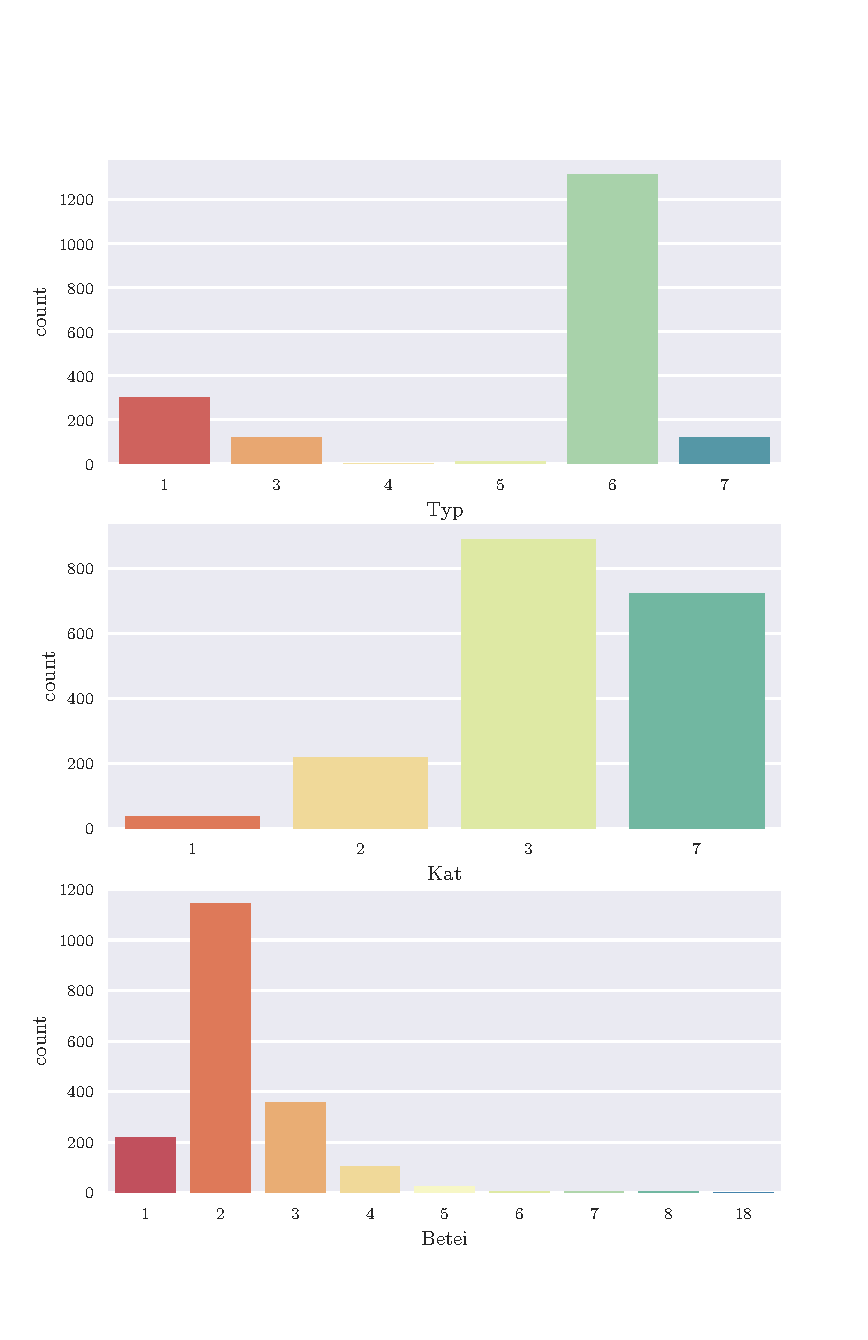
\includegraphics[scale=0.7]{../CorrAnalysis/data/BAYSIS/03_selected_01_startJam/plots/baysis_selected_count_multiple01}
    % 	\caption{Distribution of the accident category '', ...}
    % 	\label{img:appendix_baysis_selected_01_01}
    % \end{figure}
    
    % \begin{figure}[h]
    % 	\centering
    % 	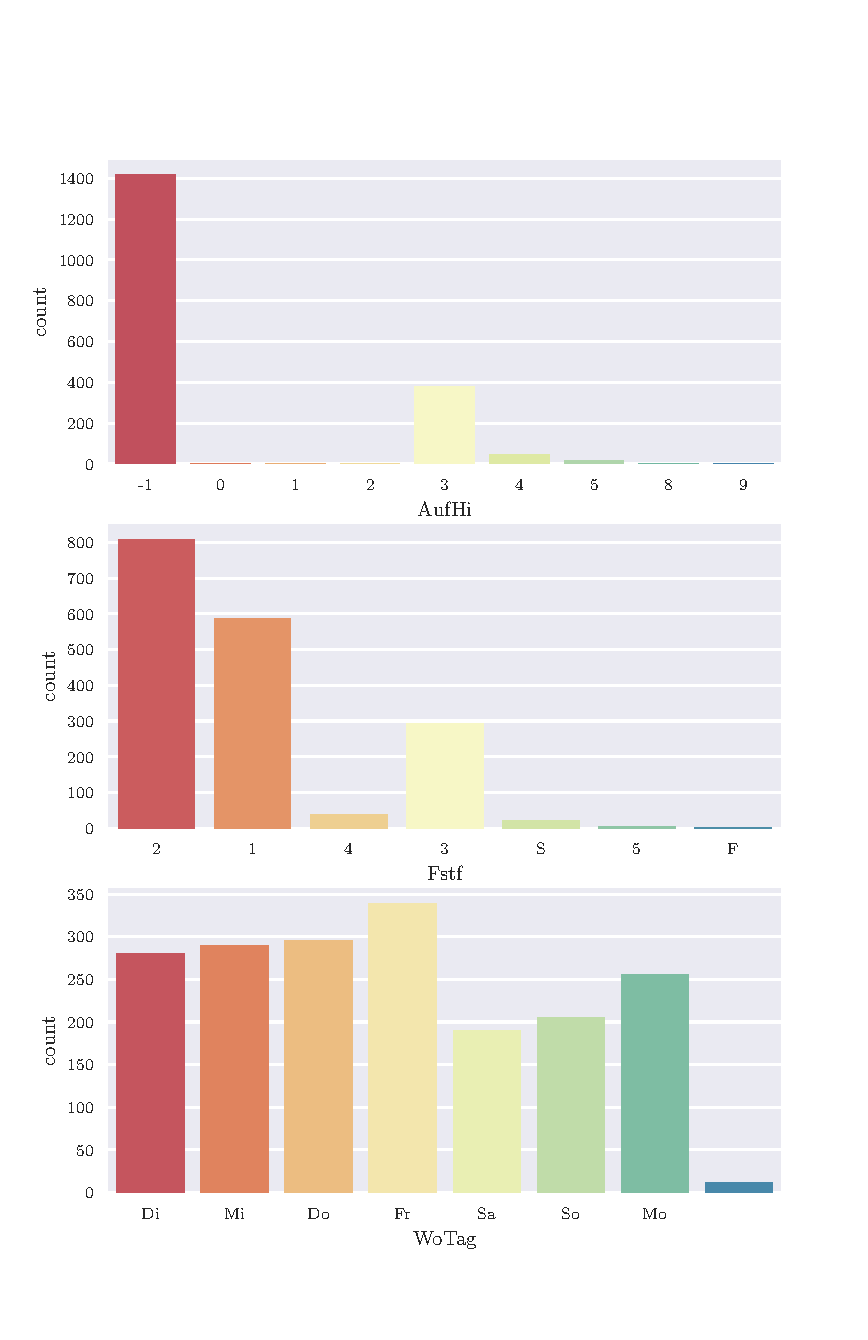
\includegraphics[scale=0.7]{../CorrAnalysis/data/BAYSIS/03_selected_01_startJam/plots/baysis_selected_count_multiple02}
    % 	\caption{Distribution of the accident category '', ..}
    % 	\label{img:appendix_baysis_selected_01_02}
    % \end{figure}
    
    % \begin{figure}[h]
    % 	\centering
    % 	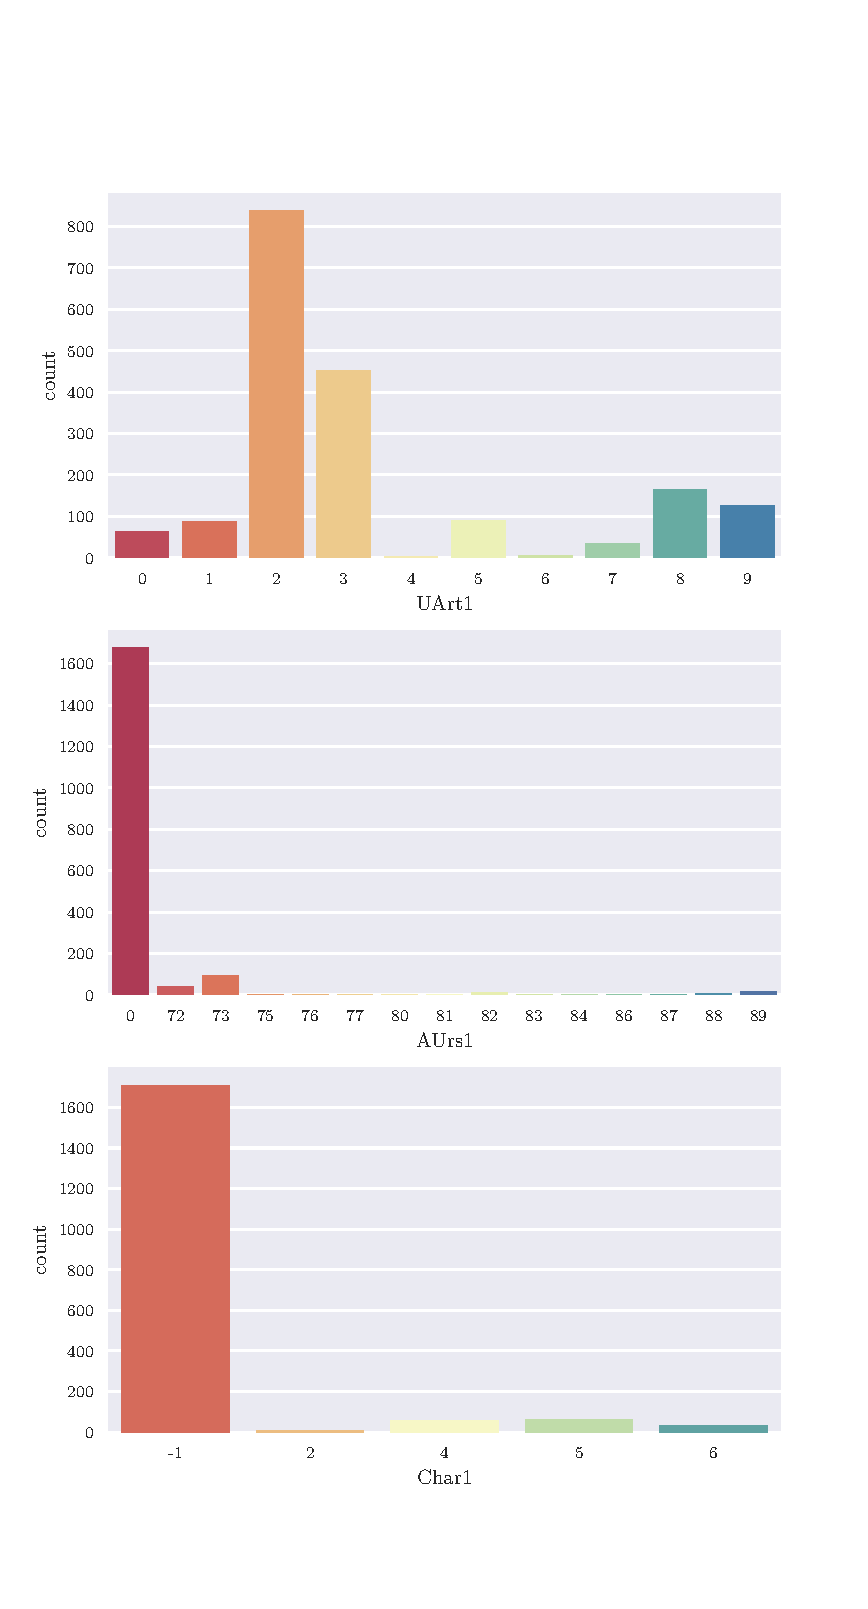
\includegraphics[scale=0.7]{../CorrAnalysis/data/BAYSIS/03_selected_01_startJam/plots/baysis_selected_count_multiple03}
    % 	\caption{Distribution of the accident category '', ..}
    % 	\label{img:appendix_baysis_selected_01_03}
    % \end{figure}
    
    % \begin{figure}[h]
    % 	\centering
    % 	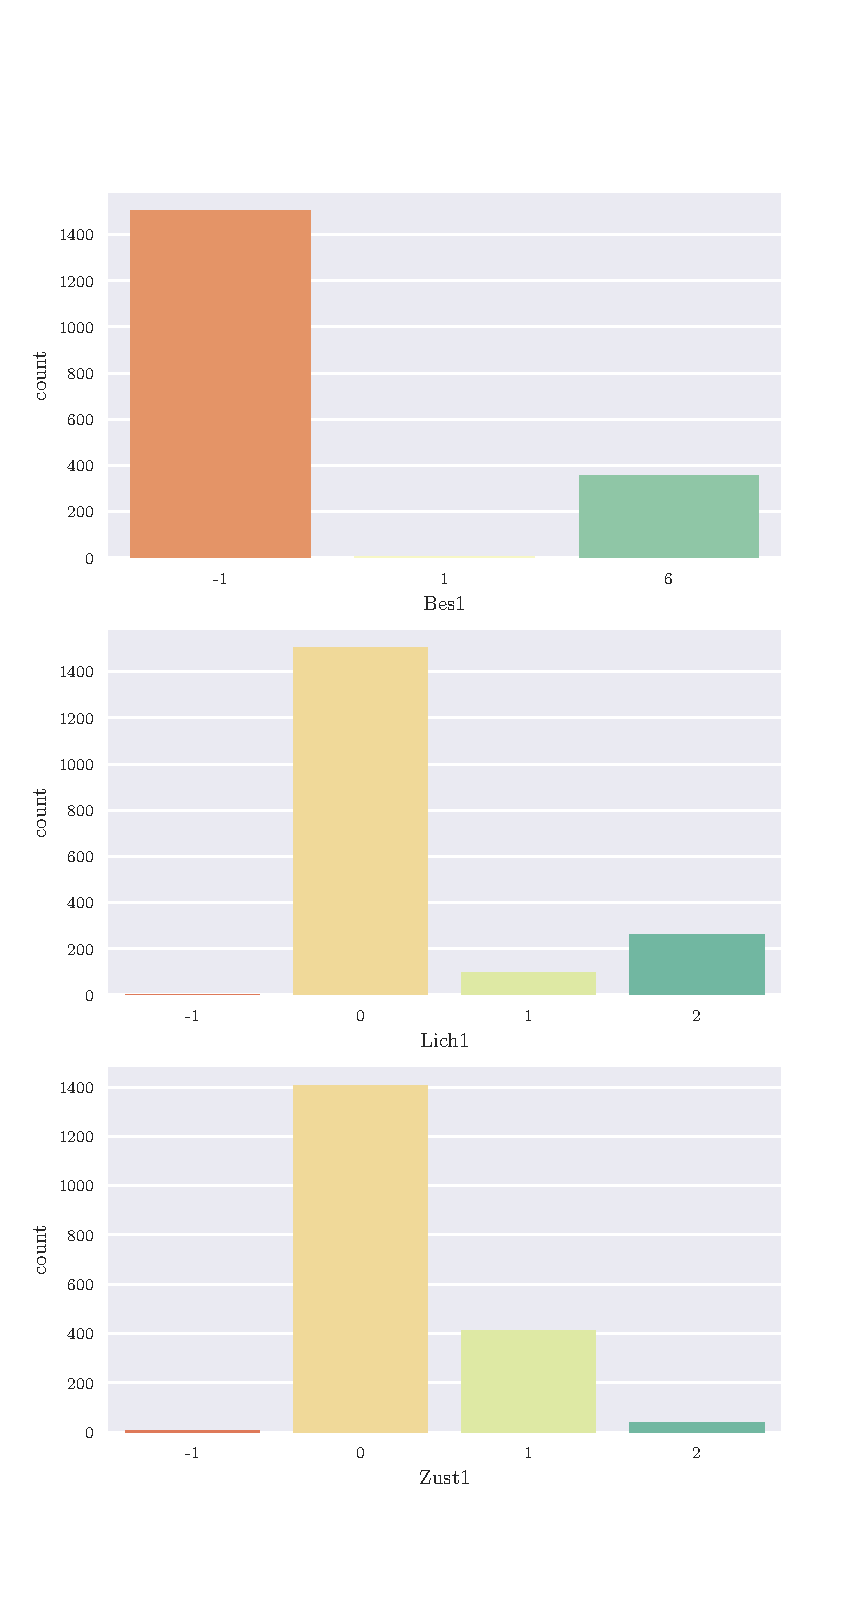
\includegraphics[scale=0.7]{../CorrAnalysis/data/BAYSIS/03_selected_01_startJam/plots/baysis_selected_count_multiple04}
    % 	\caption{Distribution of the accident category '', ...}
    % 	\label{img:appendix_baysis_selected_01_04}
    % \end{figure}
    
    % ------- BAYSIS Selected01 - Matrix --------
    % \newgeometry{left=1cm,right=1cm}
    % \begin{figure}[h]
    % 	\centering
    % 	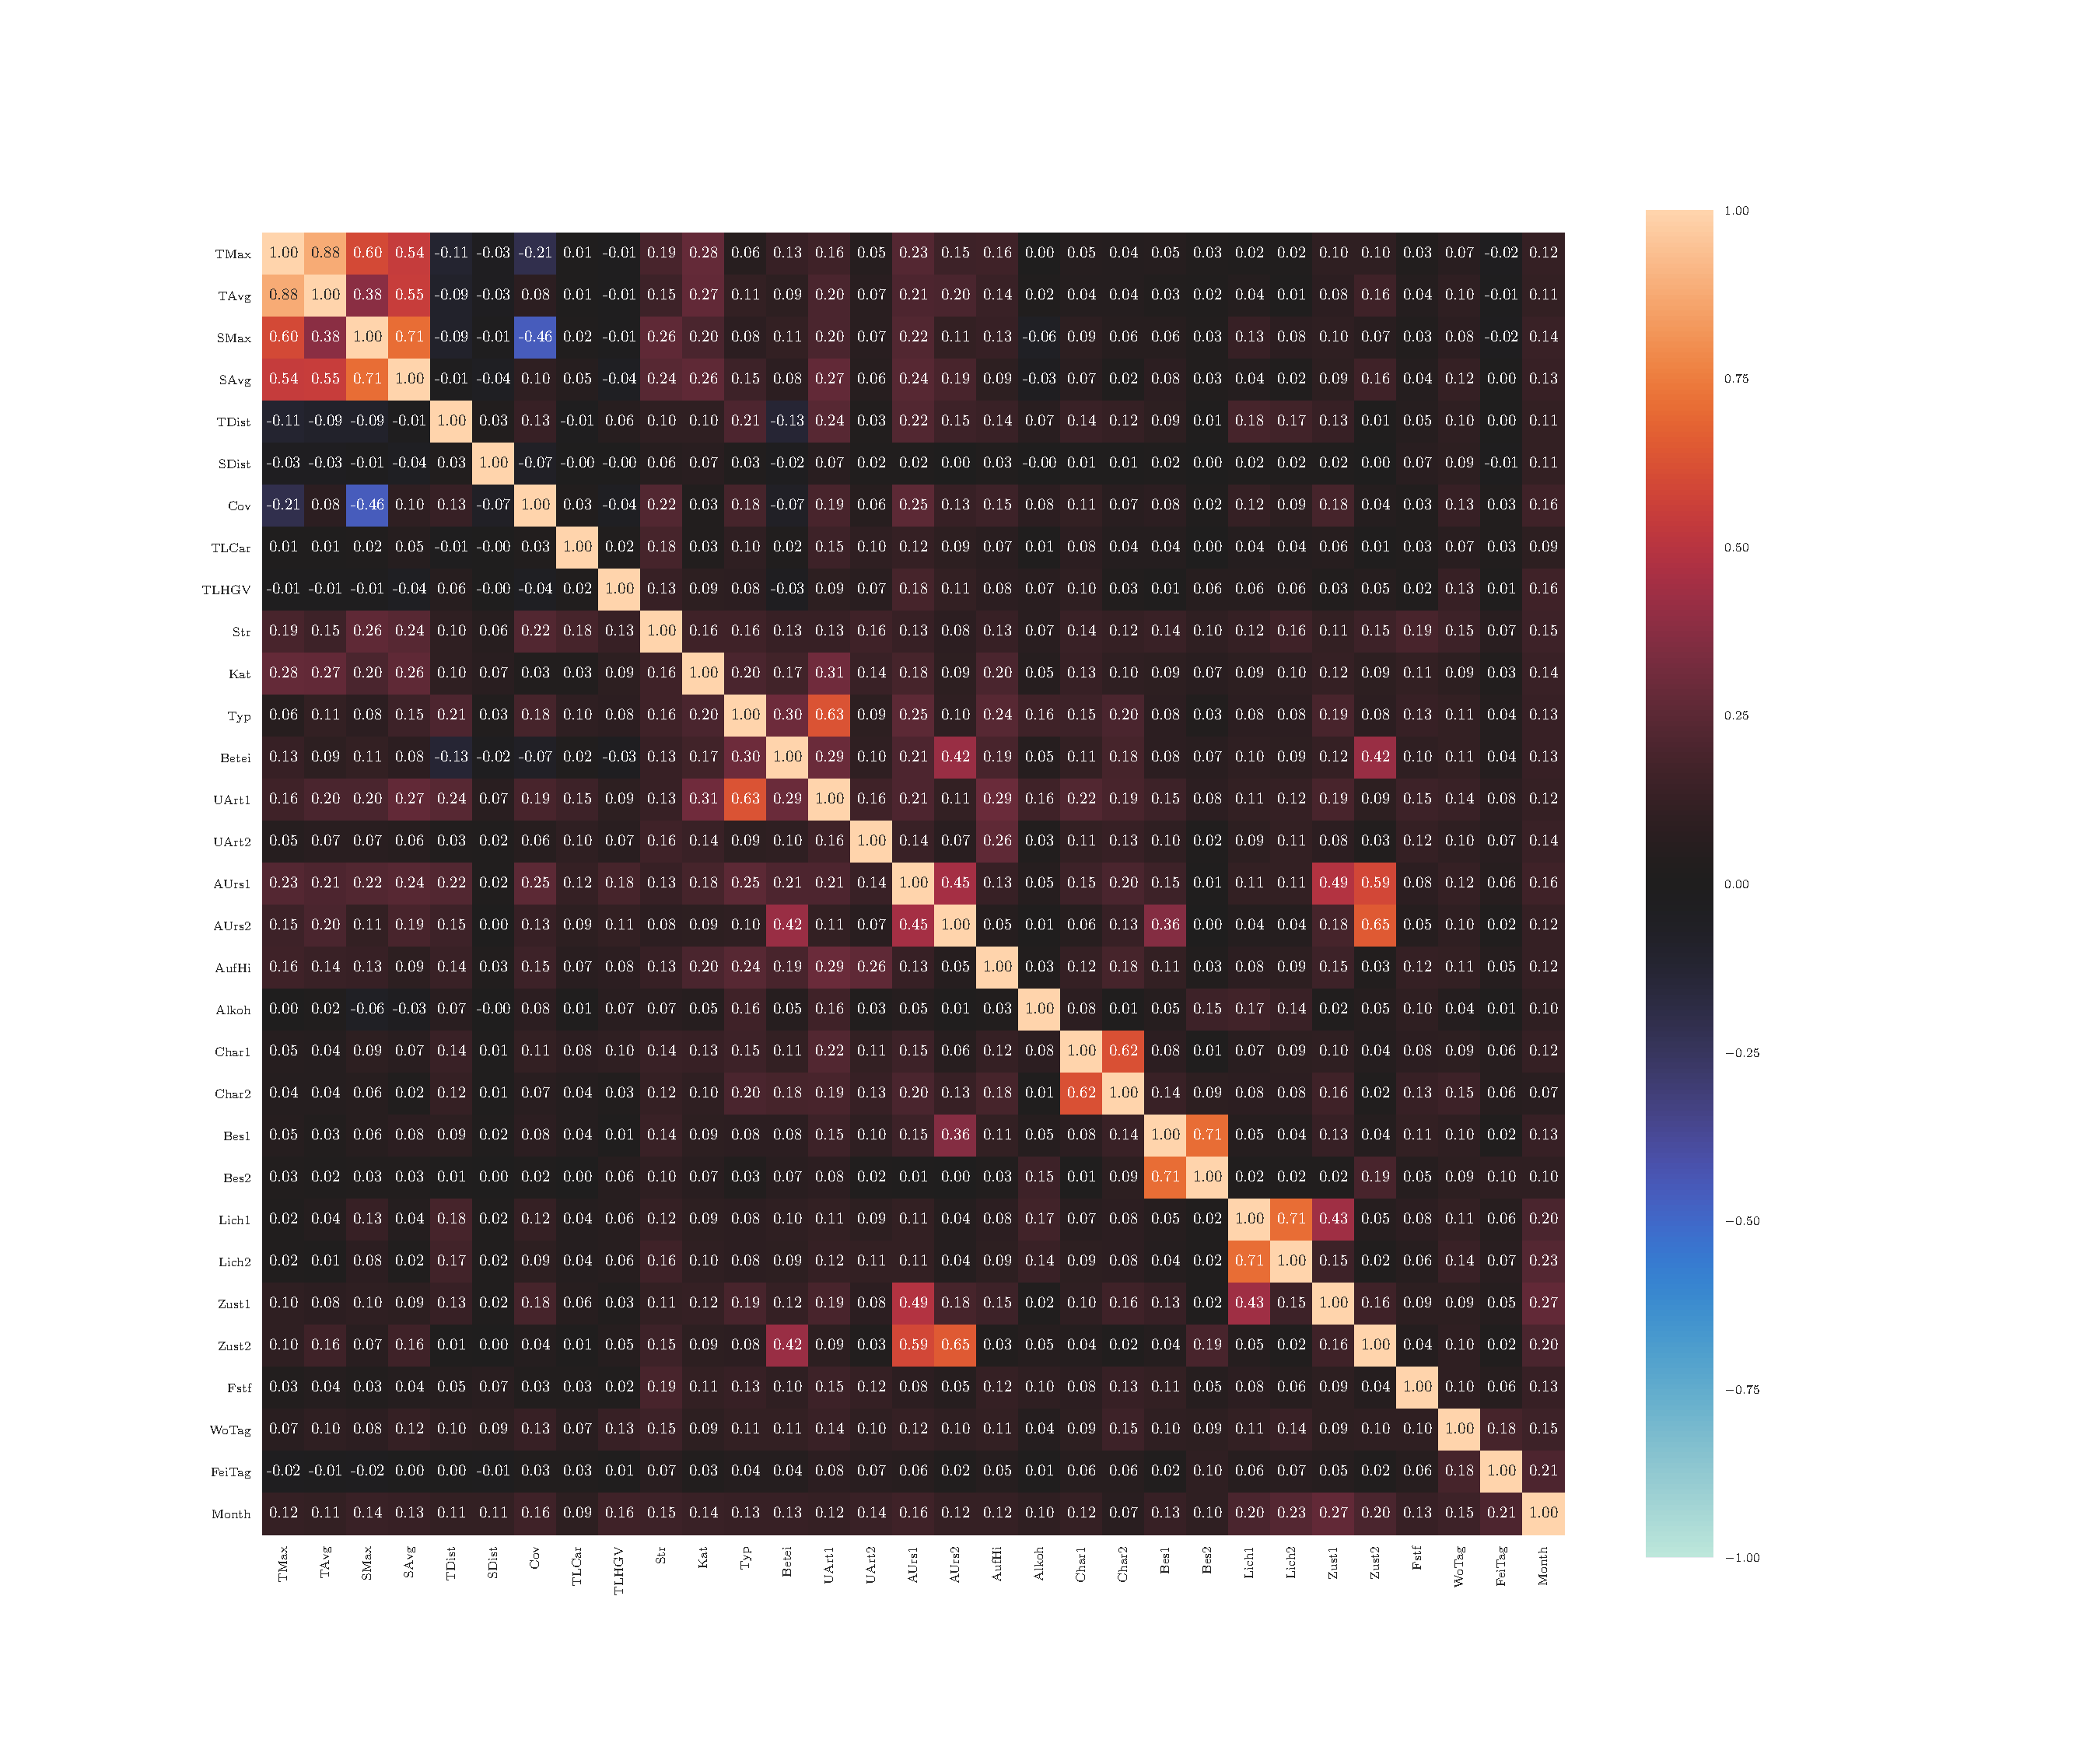
\includegraphics[scale=0.52, trim=2cm 2cm 0cm 0cm]{../CorrAnalysis/data/BAYSIS/03_selected_01_startJam/plots/baysis_selected_corr_cramers}
    % 	\caption{Correlation matrix for BAYSIS selected data (Jam Initiator), with Cramer's $V$}
    % 	\label{img:appendix_correlation_matrix_selected_startJam_cramers}
    % \end{figure}
    % \restoregeometry
    
    % \newgeometry{left=1cm,right=1cm}
    % \label{appendix_baysis_dataset_corr_theils}
    % \begin{figure}[h]
    % 	\centering
    % 	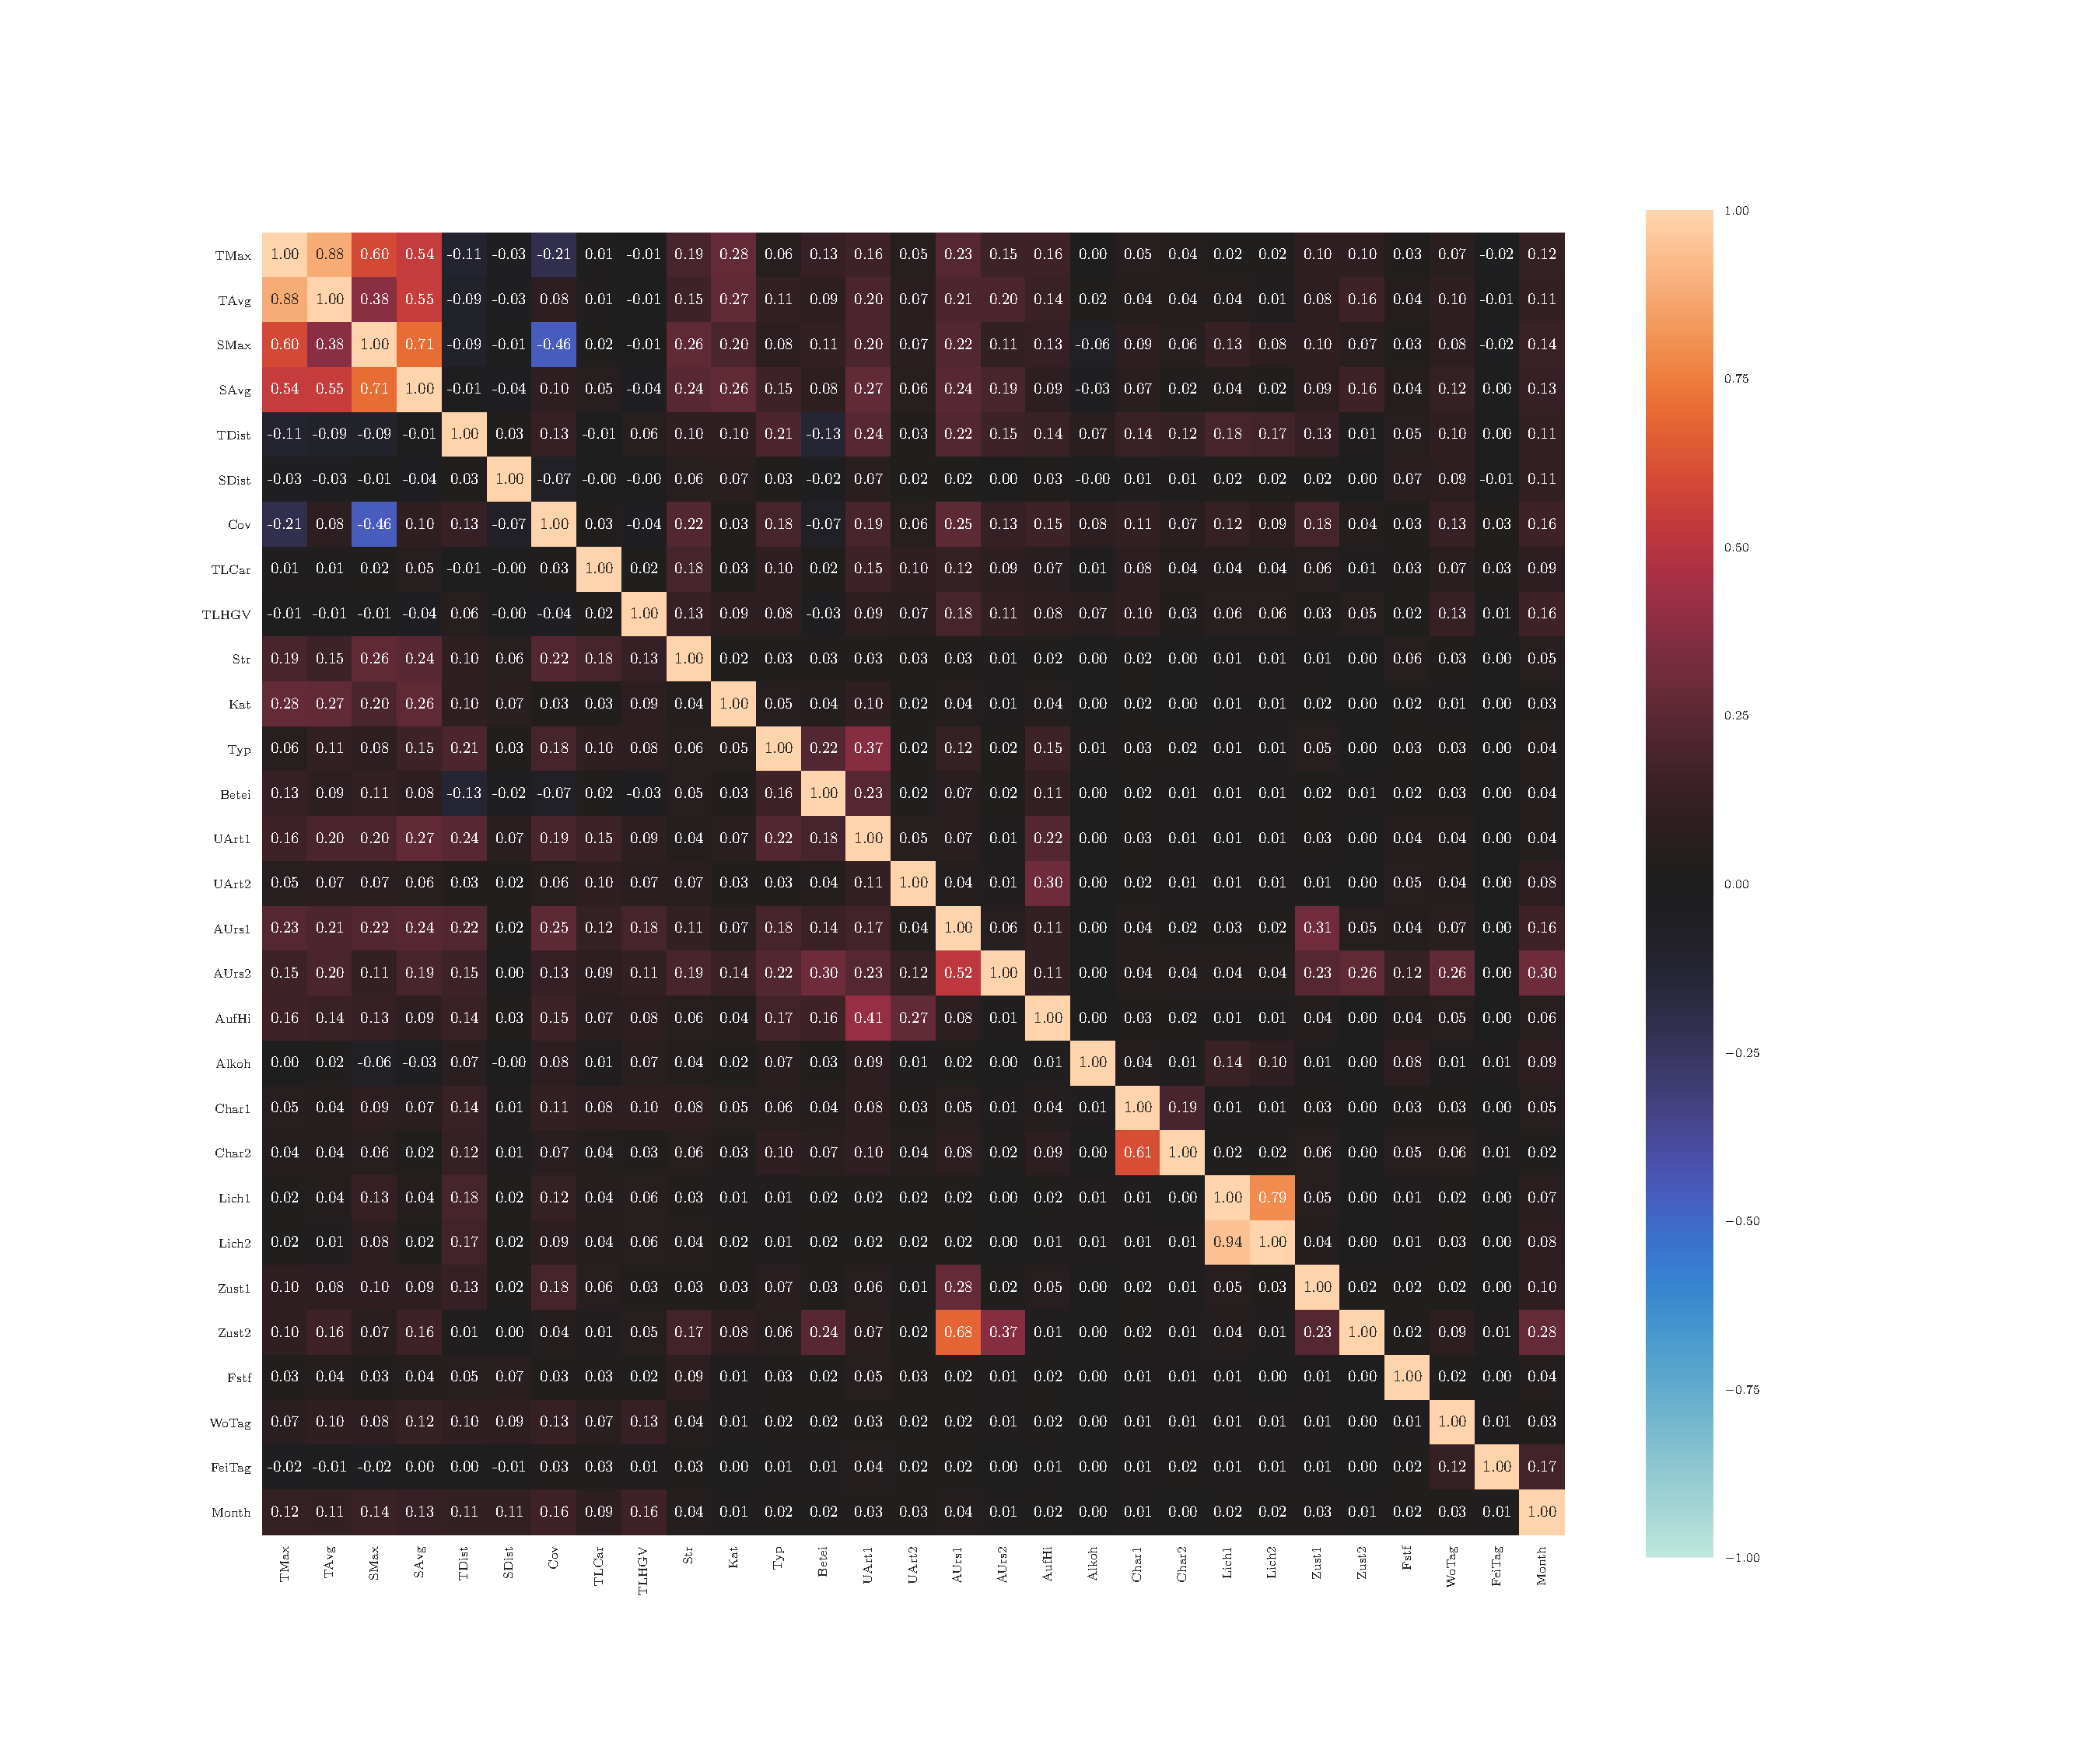
\includegraphics[scale=0.52, trim=2cm 2cm 0cm 0cm]{../CorrAnalysis/data/BAYSIS/03_selected_01_startJam/plots/baysis_selected_corr_theils}
    % 	\caption{Correlation matrix for BAYSIS selected data (Jam Initiator), with Theil's $U$}
    % 	\label{img:appendix_correlation_matrix_selected_startJam_theils}
    % \end{figure}
    % \restoregeometry
    
    % ------- BAYSIS Selected01 - Tables --------
    % \newgeometry{left=1cm,right=1cm,bottom=2cm}
    % \begin{sidewaystable}
    % 	\tiny
    % 	\setlength{\tabcolsep}{2pt}
    % 	\centering
    % 	\begin{tabular}{lrrrrrrrrrrrrrrrrrrrrrrrrrrrrrrr}
\toprule
{} &  TMax &  TAvg &  SMax &  SAvg &  TDist &  SDist &   Cov &  TLCar &  TLHGV &  Str &  Kat &  Typ &  Betei &  UArt1 &  UArt2 &  AUrs1 &  AUrs2 &  AufHi &  Alkoh &  Char1 &  Char2 &  Bes1 &  Bes2 &  Lich1 &  Lich2 &  Zust1 &  Zust2 &  Fstf &  WoTag &  FeiTag &  Month \\
\midrule
TMax   &  1.00 &  0.88 &  0.60 &  0.54 &  -0.11 &  -0.03 & -0.21 &   0.01 &  -0.01 & 0.19 & 0.28 & 0.06 &   0.13 &   0.16 &   0.05 &   0.23 &   0.15 &   0.16 &   0.00 &   0.05 &   0.04 &  0.05 &  0.03 &   0.02 &   0.02 &   0.10 &   0.10 &  0.03 &   0.07 &   -0.02 &   0.12 \\
TAvg   &  0.88 &  1.00 &  0.38 &  0.55 &  -0.09 &  -0.03 &  0.08 &   0.01 &  -0.01 & 0.15 & 0.27 & 0.11 &   0.09 &   0.20 &   0.07 &   0.21 &   0.20 &   0.14 &   0.02 &   0.04 &   0.04 &  0.03 &  0.02 &   0.04 &   0.01 &   0.08 &   0.16 &  0.04 &   0.10 &   -0.01 &   0.11 \\
SMax   &  0.60 &  0.38 &  1.00 &  0.71 &  -0.09 &  -0.01 & -0.46 &   0.02 &  -0.01 & 0.26 & 0.20 & 0.08 &   0.11 &   0.20 &   0.07 &   0.22 &   0.11 &   0.13 &  -0.06 &   0.09 &   0.06 &  0.06 &  0.03 &   0.13 &   0.08 &   0.10 &   0.07 &  0.03 &   0.08 &   -0.02 &   0.14 \\
SAvg   &  0.54 &  0.55 &  0.71 &  1.00 &  -0.01 &  -0.04 &  0.10 &   0.05 &  -0.04 & 0.24 & 0.26 & 0.15 &   0.08 &   0.27 &   0.06 &   0.24 &   0.19 &   0.09 &  -0.03 &   0.07 &   0.02 &  0.08 &  0.03 &   0.04 &   0.02 &   0.09 &   0.16 &  0.04 &   0.12 &    0.00 &   0.13 \\
TDist  & -0.11 & -0.09 & -0.09 & -0.01 &   1.00 &   0.03 &  0.13 &  -0.01 &   0.06 & 0.10 & 0.10 & 0.21 &  -0.13 &   0.24 &   0.03 &   0.22 &   0.15 &   0.14 &   0.07 &   0.14 &   0.12 &  0.09 &  0.01 &   0.18 &   0.17 &   0.13 &   0.01 &  0.05 &   0.10 &    0.00 &   0.11 \\
SDist  & -0.03 & -0.03 & -0.01 & -0.04 &   0.03 &   1.00 & -0.07 &  -0.00 &  -0.00 & 0.06 & 0.07 & 0.03 &  -0.02 &   0.07 &   0.02 &   0.02 &   0.00 &   0.03 &  -0.00 &   0.01 &   0.01 &  0.02 &  0.00 &   0.02 &   0.02 &   0.02 &   0.00 &  0.07 &   0.09 &   -0.01 &   0.11 \\
Cov    & -0.21 &  0.08 & -0.46 &  0.10 &   0.13 &  -0.07 &  1.00 &   0.03 &  -0.04 & 0.22 & 0.03 & 0.18 &  -0.07 &   0.19 &   0.06 &   0.25 &   0.13 &   0.15 &   0.08 &   0.11 &   0.07 &  0.08 &  0.02 &   0.12 &   0.09 &   0.18 &   0.04 &  0.03 &   0.13 &    0.03 &   0.16 \\
TLCar  &  0.01 &  0.01 &  0.02 &  0.05 &  -0.01 &  -0.00 &  0.03 &   1.00 &   0.02 & 0.18 & 0.03 & 0.10 &   0.02 &   0.15 &   0.10 &   0.12 &   0.09 &   0.07 &   0.01 &   0.08 &   0.04 &  0.04 &  0.00 &   0.04 &   0.04 &   0.06 &   0.01 &  0.03 &   0.07 &    0.03 &   0.09 \\
TLHGV  & -0.01 & -0.01 & -0.01 & -0.04 &   0.06 &  -0.00 & -0.04 &   0.02 &   1.00 & 0.13 & 0.09 & 0.08 &  -0.03 &   0.09 &   0.07 &   0.18 &   0.11 &   0.08 &   0.07 &   0.10 &   0.03 &  0.01 &  0.06 &   0.06 &   0.06 &   0.03 &   0.05 &  0.02 &   0.13 &    0.01 &   0.16 \\
Str    &  0.19 &  0.15 &  0.26 &  0.24 &   0.10 &   0.06 &  0.22 &   0.18 &   0.13 & 1.00 & 0.16 & 0.16 &   0.13 &   0.13 &   0.16 &   0.13 &   0.08 &   0.13 &   0.07 &   0.14 &   0.12 &  0.14 &  0.10 &   0.12 &   0.16 &   0.11 &   0.15 &  0.19 &   0.15 &    0.07 &   0.15 \\
Kat    &  0.28 &  0.27 &  0.20 &  0.26 &   0.10 &   0.07 &  0.03 &   0.03 &   0.09 & 0.16 & 1.00 & 0.20 &   0.17 &   0.31 &   0.14 &   0.18 &   0.09 &   0.20 &   0.05 &   0.13 &   0.10 &  0.09 &  0.07 &   0.09 &   0.10 &   0.12 &   0.09 &  0.11 &   0.09 &    0.03 &   0.14 \\
Typ    &  0.06 &  0.11 &  0.08 &  0.15 &   0.21 &   0.03 &  0.18 &   0.10 &   0.08 & 0.16 & 0.20 & 1.00 &   0.30 &   0.63 &   0.09 &   0.25 &   0.10 &   0.24 &   0.16 &   0.15 &   0.20 &  0.08 &  0.03 &   0.08 &   0.08 &   0.19 &   0.08 &  0.13 &   0.11 &    0.04 &   0.13 \\
Betei  &  0.13 &  0.09 &  0.11 &  0.08 &  -0.13 &  -0.02 & -0.07 &   0.02 &  -0.03 & 0.13 & 0.17 & 0.30 &   1.00 &   0.29 &   0.10 &   0.21 &   0.42 &   0.19 &   0.05 &   0.11 &   0.18 &  0.08 &  0.07 &   0.10 &   0.09 &   0.12 &   0.42 &  0.10 &   0.11 &    0.04 &   0.13 \\
UArt1  &  0.16 &  0.20 &  0.20 &  0.27 &   0.24 &   0.07 &  0.19 &   0.15 &   0.09 & 0.13 & 0.31 & 0.63 &   0.29 &   1.00 &   0.16 &   0.21 &   0.11 &   0.29 &   0.16 &   0.22 &   0.19 &  0.15 &  0.08 &   0.11 &   0.12 &   0.19 &   0.09 &  0.15 &   0.14 &    0.08 &   0.12 \\
UArt2  &  0.05 &  0.07 &  0.07 &  0.06 &   0.03 &   0.02 &  0.06 &   0.10 &   0.07 & 0.16 & 0.14 & 0.09 &   0.10 &   0.16 &   1.00 &   0.14 &   0.07 &   0.26 &   0.03 &   0.11 &   0.13 &  0.10 &  0.02 &   0.09 &   0.11 &   0.08 &   0.03 &  0.12 &   0.10 &    0.07 &   0.14 \\
AUrs1  &  0.23 &  0.21 &  0.22 &  0.24 &   0.22 &   0.02 &  0.25 &   0.12 &   0.18 & 0.13 & 0.18 & 0.25 &   0.21 &   0.21 &   0.14 &   1.00 &   0.45 &   0.13 &   0.05 &   0.15 &   0.20 &  0.15 &  0.01 &   0.11 &   0.11 &   0.49 &   0.59 &  0.08 &   0.12 &    0.06 &   0.16 \\
AUrs2  &  0.15 &  0.20 &  0.11 &  0.19 &   0.15 &   0.00 &  0.13 &   0.09 &   0.11 & 0.08 & 0.09 & 0.10 &   0.42 &   0.11 &   0.07 &   0.45 &   1.00 &   0.05 &   0.01 &   0.06 &   0.13 &  0.36 &  0.00 &   0.04 &   0.04 &   0.18 &   0.65 &  0.05 &   0.10 &    0.02 &   0.12 \\
AufHi  &  0.16 &  0.14 &  0.13 &  0.09 &   0.14 &   0.03 &  0.15 &   0.07 &   0.08 & 0.13 & 0.20 & 0.24 &   0.19 &   0.29 &   0.26 &   0.13 &   0.05 &   1.00 &   0.03 &   0.12 &   0.18 &  0.11 &  0.03 &   0.08 &   0.09 &   0.15 &   0.03 &  0.12 &   0.11 &    0.05 &   0.12 \\
Alkoh  &  0.00 &  0.02 & -0.06 & -0.03 &   0.07 &  -0.00 &  0.08 &   0.01 &   0.07 & 0.07 & 0.05 & 0.16 &   0.05 &   0.16 &   0.03 &   0.05 &   0.01 &   0.03 &   1.00 &   0.08 &   0.01 &  0.05 &  0.15 &   0.17 &   0.14 &   0.02 &   0.05 &  0.10 &   0.04 &    0.01 &   0.10 \\
Char1  &  0.05 &  0.04 &  0.09 &  0.07 &   0.14 &   0.01 &  0.11 &   0.08 &   0.10 & 0.14 & 0.13 & 0.15 &   0.11 &   0.22 &   0.11 &   0.15 &   0.06 &   0.12 &   0.08 &   1.00 &   0.62 &  0.08 &  0.01 &   0.07 &   0.09 &   0.10 &   0.04 &  0.08 &   0.09 &    0.06 &   0.12 \\
Char2  &  0.04 &  0.04 &  0.06 &  0.02 &   0.12 &   0.01 &  0.07 &   0.04 &   0.03 & 0.12 & 0.10 & 0.20 &   0.18 &   0.19 &   0.13 &   0.20 &   0.13 &   0.18 &   0.01 &   0.62 &   1.00 &  0.14 &  0.09 &   0.08 &   0.08 &   0.16 &   0.02 &  0.13 &   0.15 &    0.06 &   0.07 \\
Bes1   &  0.05 &  0.03 &  0.06 &  0.08 &   0.09 &   0.02 &  0.08 &   0.04 &   0.01 & 0.14 & 0.09 & 0.08 &   0.08 &   0.15 &   0.10 &   0.15 &   0.36 &   0.11 &   0.05 &   0.08 &   0.14 &  1.00 &  0.71 &   0.05 &   0.04 &   0.13 &   0.04 &  0.11 &   0.10 &    0.02 &   0.13 \\
Bes2   &  0.03 &  0.02 &  0.03 &  0.03 &   0.01 &   0.00 &  0.02 &   0.00 &   0.06 & 0.10 & 0.07 & 0.03 &   0.07 &   0.08 &   0.02 &   0.01 &   0.00 &   0.03 &   0.15 &   0.01 &   0.09 &  0.71 &  1.00 &   0.02 &   0.02 &   0.02 &   0.19 &  0.05 &   0.09 &    0.10 &   0.10 \\
Lich1  &  0.02 &  0.04 &  0.13 &  0.04 &   0.18 &   0.02 &  0.12 &   0.04 &   0.06 & 0.12 & 0.09 & 0.08 &   0.10 &   0.11 &   0.09 &   0.11 &   0.04 &   0.08 &   0.17 &   0.07 &   0.08 &  0.05 &  0.02 &   1.00 &   0.71 &   0.43 &   0.05 &  0.08 &   0.11 &    0.06 &   0.20 \\
Lich2  &  0.02 &  0.01 &  0.08 &  0.02 &   0.17 &   0.02 &  0.09 &   0.04 &   0.06 & 0.16 & 0.10 & 0.08 &   0.09 &   0.12 &   0.11 &   0.11 &   0.04 &   0.09 &   0.14 &   0.09 &   0.08 &  0.04 &  0.02 &   0.71 &   1.00 &   0.15 &   0.02 &  0.06 &   0.14 &    0.07 &   0.23 \\
Zust1  &  0.10 &  0.08 &  0.10 &  0.09 &   0.13 &   0.02 &  0.18 &   0.06 &   0.03 & 0.11 & 0.12 & 0.19 &   0.12 &   0.19 &   0.08 &   0.49 &   0.18 &   0.15 &   0.02 &   0.10 &   0.16 &  0.13 &  0.02 &   0.43 &   0.15 &   1.00 &   0.16 &  0.09 &   0.09 &    0.05 &   0.27 \\
Zust2  &  0.10 &  0.16 &  0.07 &  0.16 &   0.01 &   0.00 &  0.04 &   0.01 &   0.05 & 0.15 & 0.09 & 0.08 &   0.42 &   0.09 &   0.03 &   0.59 &   0.65 &   0.03 &   0.05 &   0.04 &   0.02 &  0.04 &  0.19 &   0.05 &   0.02 &   0.16 &   1.00 &  0.04 &   0.10 &    0.02 &   0.20 \\
Fstf   &  0.03 &  0.04 &  0.03 &  0.04 &   0.05 &   0.07 &  0.03 &   0.03 &   0.02 & 0.19 & 0.11 & 0.13 &   0.10 &   0.15 &   0.12 &   0.08 &   0.05 &   0.12 &   0.10 &   0.08 &   0.13 &  0.11 &  0.05 &   0.08 &   0.06 &   0.09 &   0.04 &  1.00 &   0.10 &    0.06 &   0.13 \\
WoTag  &  0.07 &  0.10 &  0.08 &  0.12 &   0.10 &   0.09 &  0.13 &   0.07 &   0.13 & 0.15 & 0.09 & 0.11 &   0.11 &   0.14 &   0.10 &   0.12 &   0.10 &   0.11 &   0.04 &   0.09 &   0.15 &  0.10 &  0.09 &   0.11 &   0.14 &   0.09 &   0.10 &  0.10 &   1.00 &    0.18 &   0.15 \\
FeiTag & -0.02 & -0.01 & -0.02 &  0.00 &   0.00 &  -0.01 &  0.03 &   0.03 &   0.01 & 0.07 & 0.03 & 0.04 &   0.04 &   0.08 &   0.07 &   0.06 &   0.02 &   0.05 &   0.01 &   0.06 &   0.06 &  0.02 &  0.10 &   0.06 &   0.07 &   0.05 &   0.02 &  0.06 &   0.18 &    1.00 &   0.21 \\
Month  &  0.12 &  0.11 &  0.14 &  0.13 &   0.11 &   0.11 &  0.16 &   0.09 &   0.16 & 0.15 & 0.14 & 0.13 &   0.13 &   0.12 &   0.14 &   0.16 &   0.12 &   0.12 &   0.10 &   0.12 &   0.07 &  0.13 &  0.10 &   0.20 &   0.23 &   0.27 &   0.20 &  0.13 &   0.15 &    0.21 &   1.00 \\
\bottomrule
\end{tabular}

    % 	\caption{Correlation matrix for BAYSIS selected data (Jam Initiator), with Cramer's $V$}
    % 	\label{table:appendix_correlation_matrix_selected_startJam_cramers}
    % \end{sidewaystable}
    
    % \newgeometry{left=1cm,right=1cm,bottom=2cm}
    % \begin{sidewaystable}
    % 	\tiny
    % 	\setlength{\tabcolsep}{2pt}
    % 	\centering
    % 	\begin{tabular}{lrrrrrrrrrrrrrrrrrrrrrrrrrrrrrrr}
\toprule
{} &  TMax &  TAvg &  SMax &  SAvg &  TDist &  SDist &   Cov &  TLCar &  TLHGV &  Str &  Kat &  Typ &  Betei &  UArt1 &  UArt2 &  AUrs1 &  AUrs2 &  AufHi &  Alkoh &  Char1 &  Char2 &  Bes1 &  Bes2 &  Lich1 &  Lich2 &  Zust1 &  Zust2 &  Fstf &  WoTag &  FeiTag &  Month \\
\midrule
TMax   &  1.00 &  0.88 &  0.60 &  0.54 &  -0.11 &  -0.03 & -0.21 &   0.01 &  -0.01 & 0.19 & 0.28 & 0.06 &   0.13 &   0.16 &   0.05 &   0.23 &   0.15 &   0.16 &   0.00 &   0.05 &   0.04 &  0.05 &  0.03 &   0.02 &   0.02 &   0.10 &   0.10 &  0.03 &   0.07 &   -0.02 &   0.12 \\
TAvg   &  0.88 &  1.00 &  0.38 &  0.55 &  -0.09 &  -0.03 &  0.08 &   0.01 &  -0.01 & 0.15 & 0.27 & 0.11 &   0.09 &   0.20 &   0.07 &   0.21 &   0.20 &   0.14 &   0.02 &   0.04 &   0.04 &  0.03 &  0.02 &   0.04 &   0.01 &   0.08 &   0.16 &  0.04 &   0.10 &   -0.01 &   0.11 \\
SMax   &  0.60 &  0.38 &  1.00 &  0.71 &  -0.09 &  -0.01 & -0.46 &   0.02 &  -0.01 & 0.26 & 0.20 & 0.08 &   0.11 &   0.20 &   0.07 &   0.22 &   0.11 &   0.13 &  -0.06 &   0.09 &   0.06 &  0.06 &  0.03 &   0.13 &   0.08 &   0.10 &   0.07 &  0.03 &   0.08 &   -0.02 &   0.14 \\
SAvg   &  0.54 &  0.55 &  0.71 &  1.00 &  -0.01 &  -0.04 &  0.10 &   0.05 &  -0.04 & 0.24 & 0.26 & 0.15 &   0.08 &   0.27 &   0.06 &   0.24 &   0.19 &   0.09 &  -0.03 &   0.07 &   0.02 &  0.08 &  0.03 &   0.04 &   0.02 &   0.09 &   0.16 &  0.04 &   0.12 &    0.00 &   0.13 \\
TDist  & -0.11 & -0.09 & -0.09 & -0.01 &   1.00 &   0.03 &  0.13 &  -0.01 &   0.06 & 0.10 & 0.10 & 0.21 &  -0.13 &   0.24 &   0.03 &   0.22 &   0.15 &   0.14 &   0.07 &   0.14 &   0.12 &  0.09 &  0.01 &   0.18 &   0.17 &   0.13 &   0.01 &  0.05 &   0.10 &    0.00 &   0.11 \\
SDist  & -0.03 & -0.03 & -0.01 & -0.04 &   0.03 &   1.00 & -0.07 &  -0.00 &  -0.00 & 0.06 & 0.07 & 0.03 &  -0.02 &   0.07 &   0.02 &   0.02 &   0.00 &   0.03 &  -0.00 &   0.01 &   0.01 &  0.02 &  0.00 &   0.02 &   0.02 &   0.02 &   0.00 &  0.07 &   0.09 &   -0.01 &   0.11 \\
Cov    & -0.21 &  0.08 & -0.46 &  0.10 &   0.13 &  -0.07 &  1.00 &   0.03 &  -0.04 & 0.22 & 0.03 & 0.18 &  -0.07 &   0.19 &   0.06 &   0.25 &   0.13 &   0.15 &   0.08 &   0.11 &   0.07 &  0.08 &  0.02 &   0.12 &   0.09 &   0.18 &   0.04 &  0.03 &   0.13 &    0.03 &   0.16 \\
TLCar  &  0.01 &  0.01 &  0.02 &  0.05 &  -0.01 &  -0.00 &  0.03 &   1.00 &   0.02 & 0.18 & 0.03 & 0.10 &   0.02 &   0.15 &   0.10 &   0.12 &   0.09 &   0.07 &   0.01 &   0.08 &   0.04 &  0.04 &  0.00 &   0.04 &   0.04 &   0.06 &   0.01 &  0.03 &   0.07 &    0.03 &   0.09 \\
TLHGV  & -0.01 & -0.01 & -0.01 & -0.04 &   0.06 &  -0.00 & -0.04 &   0.02 &   1.00 & 0.13 & 0.09 & 0.08 &  -0.03 &   0.09 &   0.07 &   0.18 &   0.11 &   0.08 &   0.07 &   0.10 &   0.03 &  0.01 &  0.06 &   0.06 &   0.06 &   0.03 &   0.05 &  0.02 &   0.13 &    0.01 &   0.16 \\
Str    &  0.19 &  0.15 &  0.26 &  0.24 &   0.10 &   0.06 &  0.22 &   0.18 &   0.13 & 1.00 & 0.02 & 0.03 &   0.03 &   0.03 &   0.03 &   0.03 &   0.01 &   0.02 &   0.00 &   0.02 &   0.00 &  0.01 &  0.00 &   0.01 &   0.01 &   0.01 &   0.00 &  0.06 &   0.03 &    0.00 &   0.05 \\
Kat    &  0.28 &  0.27 &  0.20 &  0.26 &   0.10 &   0.07 &  0.03 &   0.03 &   0.09 & 0.04 & 1.00 & 0.05 &   0.04 &   0.10 &   0.02 &   0.04 &   0.01 &   0.04 &   0.00 &   0.02 &   0.00 &  0.01 &  0.00 &   0.01 &   0.01 &   0.02 &   0.00 &  0.02 &   0.01 &    0.00 &   0.03 \\
Typ    &  0.06 &  0.11 &  0.08 &  0.15 &   0.21 &   0.03 &  0.18 &   0.10 &   0.08 & 0.06 & 0.05 & 1.00 &   0.22 &   0.37 &   0.02 &   0.12 &   0.02 &   0.15 &   0.01 &   0.03 &   0.02 &  0.01 &  0.00 &   0.01 &   0.01 &   0.05 &   0.00 &  0.03 &   0.03 &    0.00 &   0.04 \\
Betei  &  0.13 &  0.09 &  0.11 &  0.08 &  -0.13 &  -0.02 & -0.07 &   0.02 &  -0.03 & 0.05 & 0.03 & 0.16 &   1.00 &   0.23 &   0.02 &   0.07 &   0.02 &   0.11 &   0.00 &   0.02 &   0.01 &  0.01 &  0.00 &   0.01 &   0.01 &   0.02 &   0.01 &  0.02 &   0.03 &    0.00 &   0.04 \\
UArt1  &  0.16 &  0.20 &  0.20 &  0.27 &   0.24 &   0.07 &  0.19 &   0.15 &   0.09 & 0.04 & 0.07 & 0.22 &   0.18 &   1.00 &   0.05 &   0.07 &   0.01 &   0.22 &   0.00 &   0.03 &   0.01 &  0.01 &  0.00 &   0.01 &   0.01 &   0.03 &   0.00 &  0.04 &   0.04 &    0.00 &   0.04 \\
UArt2  &  0.05 &  0.07 &  0.07 &  0.06 &   0.03 &   0.02 &  0.06 &   0.10 &   0.07 & 0.07 & 0.03 & 0.03 &   0.04 &   0.11 &   1.00 &   0.04 &   0.01 &   0.30 &   0.00 &   0.02 &   0.01 &  0.02 &  0.00 &   0.01 &   0.01 &   0.01 &   0.00 &  0.05 &   0.04 &    0.00 &   0.08 \\
AUrs1  &  0.23 &  0.21 &  0.22 &  0.24 &   0.22 &   0.02 &  0.25 &   0.12 &   0.18 & 0.11 & 0.07 & 0.18 &   0.14 &   0.17 &   0.04 &   1.00 &   0.06 &   0.11 &   0.00 &   0.04 &   0.02 &  0.03 &  0.00 &   0.03 &   0.02 &   0.31 &   0.05 &  0.04 &   0.07 &    0.00 &   0.16 \\
AUrs2  &  0.15 &  0.20 &  0.11 &  0.19 &   0.15 &   0.00 &  0.13 &   0.09 &   0.11 & 0.19 & 0.14 & 0.22 &   0.30 &   0.23 &   0.12 &   0.52 &   1.00 &   0.11 &   0.00 &   0.04 &   0.04 &  0.13 &  0.00 &   0.04 &   0.04 &   0.23 &   0.26 &  0.12 &   0.26 &    0.00 &   0.30 \\
AufHi  &  0.16 &  0.14 &  0.13 &  0.09 &   0.14 &   0.03 &  0.15 &   0.07 &   0.08 & 0.06 & 0.04 & 0.17 &   0.16 &   0.41 &   0.27 &   0.08 &   0.01 &   1.00 &   0.00 &   0.03 &   0.02 &  0.01 &  0.00 &   0.01 &   0.01 &   0.04 &   0.00 &  0.04 &   0.05 &    0.00 &   0.06 \\
Alkoh  &  0.00 &  0.02 & -0.06 & -0.03 &   0.07 &  -0.00 &  0.08 &   0.01 &   0.07 & 0.04 & 0.02 & 0.07 &   0.03 &   0.09 &   0.01 &   0.02 &   0.00 &   0.01 &   1.00 &   0.04 &   0.01 &  0.01 &  0.00 &   0.14 &   0.10 &   0.01 &   0.00 &  0.08 &   0.01 &    0.01 &   0.09 \\
Char1  &  0.05 &  0.04 &  0.09 &  0.07 &   0.14 &   0.01 &  0.11 &   0.08 &   0.10 & 0.08 & 0.05 & 0.06 &   0.04 &   0.08 &   0.03 &   0.05 &   0.01 &   0.04 &   0.01 &   1.00 &   0.19 &  0.01 &  0.00 &   0.01 &   0.01 &   0.03 &   0.00 &  0.03 &   0.03 &    0.00 &   0.05 \\
Char2  &  0.04 &  0.04 &  0.06 &  0.02 &   0.12 &   0.01 &  0.07 &   0.04 &   0.03 & 0.06 & 0.03 & 0.10 &   0.07 &   0.10 &   0.04 &   0.08 &   0.02 &   0.09 &   0.00 &   0.61 &   1.00 &  0.03 &  0.00 &   0.02 &   0.02 &   0.06 &   0.00 &  0.05 &   0.06 &    0.01 &   0.02 \\
Bes1   &  0.05 &  0.03 &  0.06 &  0.08 &   0.09 &   0.02 &  0.08 &   0.04 &   0.01 & 0.05 & 0.02 & 0.01 &   0.02 &   0.05 &   0.03 &   0.04 &   0.02 &   0.03 &   0.00 &   0.01 &   0.01 &  1.00 &  0.02 &   0.01 &   0.00 &   0.02 &   0.00 &  0.04 &   0.03 &    0.00 &   0.04 \\
Bes2   &  0.03 &  0.02 &  0.03 &  0.03 &   0.01 &   0.00 &  0.02 &   0.00 &   0.06 & 0.29 & 0.19 & 0.06 &   0.20 &   0.22 &   0.03 &   0.02 &   0.00 &   0.06 &   0.00 &   0.02 &   0.00 &  0.82 &  1.00 &   0.04 &   0.04 &   0.05 &   0.00 &  0.14 &   0.26 &    0.00 &   0.28 \\
Lich1  &  0.02 &  0.04 &  0.13 &  0.04 &   0.18 &   0.02 &  0.12 &   0.04 &   0.06 & 0.03 & 0.01 & 0.01 &   0.02 &   0.02 &   0.02 &   0.02 &   0.00 &   0.02 &   0.01 &   0.01 &   0.00 &  0.00 &  0.00 &   1.00 &   0.79 &   0.05 &   0.00 &  0.01 &   0.02 &    0.00 &   0.07 \\
Lich2  &  0.02 &  0.01 &  0.08 &  0.02 &   0.17 &   0.02 &  0.09 &   0.04 &   0.06 & 0.04 & 0.02 & 0.01 &   0.02 &   0.02 &   0.02 &   0.02 &   0.00 &   0.01 &   0.01 &   0.01 &   0.01 &  0.00 &  0.00 &   0.94 &   1.00 &   0.04 &   0.00 &  0.01 &   0.03 &    0.00 &   0.08 \\
Zust1  &  0.10 &  0.08 &  0.10 &  0.09 &   0.13 &   0.02 &  0.18 &   0.06 &   0.03 & 0.03 & 0.03 & 0.07 &   0.03 &   0.06 &   0.01 &   0.28 &   0.02 &   0.05 &   0.00 &   0.02 &   0.01 &  0.01 &  0.00 &   0.05 &   0.03 &   1.00 &   0.02 &  0.02 &   0.02 &    0.00 &   0.10 \\
Zust2  &  0.10 &  0.16 &  0.07 &  0.16 &   0.01 &   0.00 &  0.04 &   0.01 &   0.05 & 0.17 & 0.08 & 0.06 &   0.24 &   0.07 &   0.02 &   0.68 &   0.37 &   0.01 &   0.00 &   0.02 &   0.01 &  0.03 &  0.00 &   0.04 &   0.01 &   0.23 &   1.00 &  0.02 &   0.09 &    0.01 &   0.28 \\
Fstf   &  0.03 &  0.04 &  0.03 &  0.04 &   0.05 &   0.07 &  0.03 &   0.03 &   0.02 & 0.09 & 0.01 & 0.03 &   0.02 &   0.05 &   0.03 &   0.02 &   0.01 &   0.02 &   0.00 &   0.01 &   0.01 &  0.01 &  0.00 &   0.01 &   0.00 &   0.01 &   0.00 &  1.00 &   0.02 &    0.00 &   0.04 \\
WoTag  &  0.07 &  0.10 &  0.08 &  0.12 &   0.10 &   0.09 &  0.13 &   0.07 &   0.13 & 0.04 & 0.01 & 0.02 &   0.02 &   0.03 &   0.02 &   0.02 &   0.01 &   0.02 &   0.00 &   0.01 &   0.01 &  0.01 &  0.00 &   0.01 &   0.01 &   0.01 &   0.00 &  0.01 &   1.00 &    0.01 &   0.03 \\
FeiTag & -0.02 & -0.01 & -0.02 &  0.00 &   0.00 &  -0.01 &  0.03 &   0.03 &   0.01 & 0.03 & 0.00 & 0.01 &   0.01 &   0.04 &   0.02 &   0.02 &   0.00 &   0.01 &   0.00 &   0.01 &   0.02 &  0.00 &  0.00 &   0.01 &   0.01 &   0.01 &   0.00 &  0.02 &   0.12 &    1.00 &   0.17 \\
Month  &  0.12 &  0.11 &  0.14 &  0.13 &   0.11 &   0.11 &  0.16 &   0.09 &   0.16 & 0.04 & 0.01 & 0.02 &   0.02 &   0.03 &   0.03 &   0.04 &   0.01 &   0.02 &   0.00 &   0.01 &   0.00 &  0.01 &  0.00 &   0.02 &   0.02 &   0.03 &   0.01 &  0.02 &   0.03 &    0.01 &   1.00 \\
\bottomrule
\end{tabular}

    % 	\caption{Correlation matrix for BAYSIS selected data (Jam Initiator), with Theil's $U$}
    % 	\label{table:appendix_correlation_matrix_selected_startJam_cramers}
    % \end{sidewaystable}
    
    % \newgeometry{left=1cm,right=1cm,bottom=2cm}
    % \begin{sidewaystable}
    % 	\tiny
    % 	\setlength{\tabcolsep}{2pt}
    % 	\centering
    % 	\begin{tabular}{lrrrrrrrrrrrrrrrrrrrrrrrrrrrrrrr}
\toprule
{} &  TMax &  TAvg &  SMax &  SAvg &  TDist &  SDist &   Cov &  TLCar &  TLHGV &   Str &   Kat &   Typ &  Betei &  UArt1 &  UArt2 &  AUrs1 &  AUrs2 &  AufHi &  Alkoh &  Char1 &  Char2 &  Bes1 &  Bes2 &  Lich1 &  Lich2 &  Zust1 &  Zust2 &  Fstf &  WoTag &  FeiTag &  Month \\
\midrule
TMax   &   nan & 0.000 & 0.000 & 0.000 &  0.002 &  0.361 & 0.000 &  0.696 &  0.883 & 0.000 & 0.000 & 0.000 &  0.000 &  0.000 &  0.000 &  0.000 &  0.000 &  0.000 &  0.975 &  0.000 &  0.000 & 0.000 & 0.000 &  0.000 &  0.000 &  0.000 &  0.000 & 0.302 &  0.000 &   0.569 &  0.000 \\
TAvg   & 0.000 &   nan & 0.000 & 0.000 &  0.011 &  0.334 & 0.023 &  0.684 &  0.718 & 0.000 & 0.000 & 0.000 &  0.001 &  0.000 &  0.000 &  0.000 &  0.000 &  0.000 &  0.528 &  0.000 &  0.000 & 0.000 & 0.000 &  0.000 &  0.000 &  0.000 &  0.000 & 0.193 &  0.000 &   0.709 &  0.000 \\
SMax   & 0.000 & 0.000 &   nan & 0.000 &  0.017 &  0.865 & 0.000 &  0.625 &  0.874 & 0.000 & 0.000 & 0.000 &  0.000 &  0.000 &  0.000 &  0.000 &  0.000 &  0.000 &  0.119 &  0.000 &  0.000 & 0.000 & 0.000 &  0.000 &  0.000 &  0.000 &  0.000 & 0.321 &  0.000 &   0.581 &  0.000 \\
SAvg   & 0.000 & 0.000 & 0.000 &   nan &  0.727 &  0.273 & 0.006 &  0.179 &  0.274 & 0.000 & 0.000 & 0.000 &  0.003 &  0.000 &  0.000 &  0.000 &  0.000 &  0.000 &  0.466 &  0.000 &  0.000 & 0.000 & 0.000 &  0.000 &  0.000 &  0.000 &  0.000 & 0.182 &  0.000 &   0.960 &  0.000 \\
TDist  & 0.002 & 0.011 & 0.017 & 0.727 &    nan &  0.448 & 0.000 &  0.830 &  0.108 & 0.000 & 0.000 & 0.000 &  0.000 &  0.000 &  0.000 &  0.000 &  0.000 &  0.000 &  0.043 &  0.000 &  0.000 & 0.000 & 0.000 &  0.000 &  0.000 &  0.000 &  0.000 & 0.095 &  0.000 &   0.968 &  0.000 \\
SDist  & 0.361 & 0.334 & 0.865 & 0.273 &  0.448 &    nan & 0.061 &  0.946 &  0.904 & 0.000 & 0.000 & 0.000 &  0.615 &  0.000 &  0.000 &  0.000 &  0.130 &  0.000 &  0.901 &  0.000 &  0.000 & 0.000 & 0.000 &  0.000 &  0.000 &  0.000 &  0.000 & 0.044 &  0.000 &   0.757 &  0.000 \\
Cov    & 0.000 & 0.023 & 0.000 & 0.006 &  0.000 &  0.061 &   nan &  0.481 &  0.259 & 0.000 & 0.000 & 0.000 &  0.010 &  0.000 &  0.000 &  0.000 &  0.000 &  0.000 &  0.023 &  0.000 &  0.000 & 0.000 & 0.000 &  0.000 &  0.000 &  0.000 &  0.000 & 0.242 &  0.000 &   0.331 &  0.000 \\
TLCar  & 0.696 & 0.684 & 0.625 & 0.179 &  0.830 &  0.946 & 0.481 &    nan &  0.591 & 0.000 & 0.000 & 0.000 &  0.397 &  0.000 &  0.000 &  0.000 &  0.000 &  0.000 &  0.807 &  0.000 &  0.000 & 0.000 & 0.000 &  0.000 &  0.000 &  0.000 &  0.000 & 0.311 &  0.000 &   0.359 &  0.000 \\
TLHGV  & 0.883 & 0.718 & 0.874 & 0.274 &  0.108 &  0.904 & 0.259 &  0.591 &    nan & 0.000 & 0.000 & 0.000 &  0.319 &  0.000 &  0.000 &  0.000 &  0.000 &  0.000 &  0.043 &  0.000 &  0.000 & 0.000 & 0.000 &  0.000 &  0.000 &  0.000 &  0.000 & 0.437 &  0.000 &   0.859 &  0.000 \\
Str    & 0.000 & 0.000 & 0.000 & 0.000 &  0.000 &  0.000 & 0.000 &  0.000 &  0.000 &   nan & 0.042 & 0.021 &  0.807 &  0.804 &  0.015 &  0.711 &  1.000 &  0.605 &  0.995 &  0.227 &  0.698 & 0.319 & 0.897 &  0.751 &  0.108 &  0.913 &  0.186 & 0.000 &  0.120 &   0.995 &  0.016 \\
Kat    & 0.000 & 0.000 & 0.000 & 0.000 &  0.000 &  0.000 & 0.000 &  0.000 &  0.000 & 0.042 &   nan & 0.000 &  0.000 &  0.000 &  0.004 &  0.000 &  0.532 &  0.000 &  0.515 &  0.000 &  0.036 & 0.043 & 0.348 &  0.049 &  0.028 &  0.000 &  0.123 & 0.161 &  0.689 &   0.844 &  0.038 \\
Typ    & 0.000 & 0.000 & 0.000 & 0.000 &  0.000 &  0.000 & 0.000 &  0.000 &  0.000 & 0.021 & 0.000 &   nan &  0.000 &  0.000 &  0.617 &  0.000 &  0.167 &  0.000 &  0.001 &  0.000 &  0.000 & 0.548 & 0.990 &  0.587 &  0.435 &  0.000 &  0.432 & 0.002 &  0.077 &   0.930 &  0.248 \\
Betei  & 0.000 & 0.001 & 0.000 & 0.003 &  0.000 &  0.615 & 0.010 &  0.397 &  0.319 & 0.807 & 0.000 & 0.000 &    nan &  0.000 &  0.541 &  0.000 &  0.000 &  0.000 &  0.980 &  0.317 &  0.002 & 0.823 & 0.880 &  0.492 &  0.599 &  0.054 &  0.000 & 0.594 &  0.144 &   0.992 &  0.186 \\
UArt1  & 0.000 & 0.000 & 0.000 & 0.000 &  0.000 &  0.000 & 0.000 &  0.000 &  0.000 & 0.804 & 0.000 & 0.000 &  0.000 &    nan &  0.000 &  0.000 &  0.279 &  0.000 &  0.018 &  0.000 &  0.001 & 0.011 & 0.883 &  0.284 &  0.204 &  0.000 &  0.755 & 0.000 &  0.002 &   0.819 &  0.398 \\
UArt2  & 0.000 & 0.000 & 0.000 & 0.000 &  0.000 &  0.000 & 0.000 &  0.000 &  0.000 & 0.015 & 0.004 & 0.617 &  0.541 &  0.000 &    nan &  0.021 &  0.997 &  0.000 &  0.999 &  0.114 &  0.079 & 0.367 & 1.000 &  0.581 &  0.158 &  0.836 &  0.996 & 0.011 &  0.449 &   0.778 &  0.008 \\
AUrs1  & 0.000 & 0.000 & 0.000 & 0.000 &  0.000 &  0.000 & 0.000 &  0.000 &  0.000 & 0.711 & 0.000 & 0.000 &  0.000 &  0.000 &  0.021 &    nan &  0.000 &  0.158 &  0.999 &  0.013 &  0.003 & 0.042 & 1.000 &  0.769 &  0.771 &  0.000 &  0.000 & 1.000 &  0.468 &   0.998 &  0.000 \\
AUrs2  & 0.000 & 0.000 & 0.000 & 0.000 &  0.000 &  0.130 & 0.000 &  0.000 &  0.000 & 1.000 & 0.532 & 0.167 &  0.000 &  0.279 &  0.997 &  0.000 &    nan &  1.000 &  1.000 &  0.996 &  0.058 & 0.000 & 1.000 &  1.000 &  0.997 &  0.000 &  0.000 & 1.000 &  0.316 &   1.000 &  0.378 \\
AufHi  & 0.000 & 0.000 & 0.000 & 0.000 &  0.000 &  0.000 & 0.000 &  0.000 &  0.000 & 0.605 & 0.000 & 0.000 &  0.000 &  0.000 &  0.000 &  0.158 &  1.000 &    nan &  0.999 &  0.035 &  0.002 & 0.338 & 1.000 &  0.910 &  0.773 &  0.002 &  0.999 & 0.020 &  0.117 &   0.975 &  0.521 \\
Alkoh  & 0.975 & 0.528 & 0.119 & 0.466 &  0.043 &  0.901 & 0.023 &  0.807 &  0.043 & 0.995 & 0.515 & 0.001 &  0.980 &  0.018 &  0.999 &  0.999 &  1.000 &  0.999 &    nan &  0.296 &  0.886 & 0.411 & 0.000 &  0.000 &  0.001 &  0.961 &  0.198 & 0.308 &  0.993 &   0.778 &  0.719 \\
Char1  & 0.000 & 0.000 & 0.000 & 0.000 &  0.000 &  0.000 & 0.000 &  0.000 &  0.000 & 0.227 & 0.000 & 0.000 &  0.317 &  0.000 &  0.114 &  0.013 &  0.996 &  0.035 &  0.296 &    nan &  0.000 & 0.207 & 0.998 &  0.380 &  0.139 &  0.026 &  0.909 & 0.908 &  0.534 &   0.653 &  0.511 \\
Char2  & 0.000 & 0.000 & 0.000 & 0.000 &  0.000 &  0.000 & 0.000 &  0.000 &  0.000 & 0.698 & 0.036 & 0.000 &  0.002 &  0.001 &  0.079 &  0.003 &  0.058 &  0.002 &  0.886 &  0.000 &    nan & 0.001 & 0.015 &  0.148 &  0.078 &  0.000 &  0.632 & 0.084 &  0.011 &   0.079 &  0.969 \\
Bes1   & 0.000 & 0.000 & 0.000 & 0.000 &  0.000 &  0.000 & 0.000 &  0.000 &  0.000 & 0.319 & 0.043 & 0.548 &  0.823 &  0.011 &  0.367 &  0.042 &  0.000 &  0.338 &  0.411 &  0.207 &  0.001 &   nan & 0.000 &  0.702 &  0.642 &  0.000 &  0.565 & 0.126 &  0.376 &   0.882 &  0.237 \\
Bes2   & 0.000 & 0.000 & 0.000 & 0.000 &  0.000 &  0.000 & 0.000 &  0.000 &  0.000 & 0.897 & 0.348 & 0.990 &  0.880 &  0.883 &  1.000 &  1.000 &  1.000 &  1.000 &  0.000 &  0.998 &  0.015 & 0.000 &   nan &  0.953 &  0.847 &  0.937 &  0.000 & 0.964 &  0.501 &   0.007 &  0.761 \\
Lich1  & 0.000 & 0.000 & 0.000 & 0.000 &  0.000 &  0.000 & 0.000 &  0.000 &  0.000 & 0.751 & 0.049 & 0.587 &  0.492 &  0.284 &  0.581 &  0.769 &  1.000 &  0.910 &  0.000 &  0.380 &  0.148 & 0.702 & 0.953 &    nan &  0.000 &  0.000 &  0.560 & 0.813 &  0.217 &   0.483 &  0.000 \\
Lich2  & 0.000 & 0.000 & 0.000 & 0.000 &  0.000 &  0.000 & 0.000 &  0.000 &  0.000 & 0.108 & 0.028 & 0.435 &  0.599 &  0.204 &  0.158 &  0.771 &  0.997 &  0.773 &  0.001 &  0.139 &  0.078 & 0.642 & 0.847 &  0.000 &    nan &  0.000 &  0.798 & 0.968 &  0.004 &   0.115 &  0.000 \\
Zust1  & 0.000 & 0.000 & 0.000 & 0.000 &  0.000 &  0.000 & 0.000 &  0.000 &  0.000 & 0.913 & 0.000 & 0.000 &  0.054 &  0.000 &  0.836 &  0.000 &  0.000 &  0.002 &  0.961 &  0.026 &  0.000 & 0.000 & 0.937 &  0.000 &  0.000 &    nan &  0.000 & 0.696 &  0.609 &   0.586 &  0.000 \\
Zust2  & 0.000 & 0.000 & 0.000 & 0.000 &  0.000 &  0.000 & 0.000 &  0.000 &  0.000 & 0.186 & 0.123 & 0.432 &  0.000 &  0.755 &  0.996 &  0.000 &  0.000 &  0.999 &  0.198 &  0.909 &  0.632 & 0.565 & 0.000 &  0.560 &  0.798 &  0.000 &    nan & 0.990 &  0.426 &   0.533 &  0.001 \\
Fstf   & 0.302 & 0.193 & 0.321 & 0.182 &  0.095 &  0.044 & 0.242 &  0.311 &  0.437 & 0.000 & 0.161 & 0.002 &  0.594 &  0.000 &  0.011 &  1.000 &  1.000 &  0.020 &  0.308 &  0.908 &  0.084 & 0.126 & 0.964 &  0.813 &  0.968 &  0.696 &  0.990 &   nan &  0.414 &   0.873 &  0.164 \\
WoTag  & 0.000 & 0.000 & 0.000 & 0.000 &  0.000 &  0.000 & 0.000 &  0.000 &  0.000 & 0.120 & 0.689 & 0.077 &  0.144 &  0.002 &  0.449 &  0.468 &  0.316 &  0.117 &  0.993 &  0.534 &  0.011 & 0.376 & 0.501 &  0.217 &  0.004 &  0.609 &  0.426 & 0.414 &    nan &   0.001 &  0.002 \\
FeiTag & 0.569 & 0.709 & 0.581 & 0.960 &  0.968 &  0.757 & 0.331 &  0.359 &  0.859 & 0.995 & 0.844 & 0.930 &  0.992 &  0.819 &  0.778 &  0.998 &  1.000 &  0.975 &  0.778 &  0.653 &  0.079 & 0.882 & 0.007 &  0.483 &  0.115 &  0.586 &  0.533 & 0.873 &  0.001 &     nan &  0.000 \\
Month  & 0.000 & 0.000 & 0.000 & 0.000 &  0.000 &  0.000 & 0.000 &  0.000 &  0.000 & 0.016 & 0.038 & 0.248 &  0.186 &  0.398 &  0.008 &  0.000 &  0.378 &  0.521 &  0.719 &  0.511 &  0.969 & 0.237 & 0.761 &  0.000 &  0.000 &  0.000 &  0.001 & 0.164 &  0.002 &   0.000 &    nan \\
\bottomrule
\end{tabular}

    % 	\caption{Significancy matrix for BAYSIS selected data (Jam Initiator)}
    % 	\label{table:appendix_significancy_matrix_selected_startJam}
    % \end{sidewaystable}
    % \restoregeometry
    
    % \newgeometry{left=1cm,right=1cm,bottom=2cm}
    % \begin{sidewaystable}
    % 	\tiny
    % 	\setlength{\tabcolsep}{2pt}
    % 	\centering
    % 	\begin{tabular}{llllllllllllllllllllllllllllllll}
\toprule
{} &      TMax &      TAvg &      SMax &      SAvg &     TDist &     SDist &       Cov &     TLCar &     TLHGV &     Str &     Kat &     Typ &   Betei &   UArt1 &   UArt2 &   AUrs1 &   AUrs2 &   AufHi &     Alkoh &   Char1 &   Char2 &    Bes1 &    Bes2 &   Lich1 &   Lich2 &   Zust1 &   Zust2 &    Fstf &   WoTag &  FeiTag &   Month \\
\midrule
TMax   &       NaN &       $r$ &       $r$ &       $r$ &       $r$ &       $r$ &       $r$ &       $r$ &       $r$ &  $\eta$ &  $\eta$ &  $\eta$ &  $\tau$ &  $\eta$ &  $\eta$ &  $\eta$ &  $\eta$ &  $\eta$ &  $r_{pq}$ &  $\eta$ &  $\eta$ &  $\eta$ &  $\eta$ &  $\eta$ &  $\eta$ &  $\eta$ &  $\eta$ &  $\tau$ &  $\eta$ &  $\tau$ &  $\eta$ \\
TAvg   &       $r$ &       NaN &       $r$ &       $r$ &       $r$ &       $r$ &       $r$ &       $r$ &       $r$ &  $\eta$ &  $\eta$ &  $\eta$ &  $\tau$ &  $\eta$ &  $\eta$ &  $\eta$ &  $\eta$ &  $\eta$ &  $r_{pq}$ &  $\eta$ &  $\eta$ &  $\eta$ &  $\eta$ &  $\eta$ &  $\eta$ &  $\eta$ &  $\eta$ &  $\tau$ &  $\eta$ &  $\tau$ &  $\eta$ \\
SMax   &       $r$ &       $r$ &       NaN &       $r$ &       $r$ &       $r$ &       $r$ &       $r$ &       $r$ &  $\eta$ &  $\eta$ &  $\eta$ &  $\tau$ &  $\eta$ &  $\eta$ &  $\eta$ &  $\eta$ &  $\eta$ &  $r_{pq}$ &  $\eta$ &  $\eta$ &  $\eta$ &  $\eta$ &  $\eta$ &  $\eta$ &  $\eta$ &  $\eta$ &  $\tau$ &  $\eta$ &  $\tau$ &  $\eta$ \\
SAvg   &       $r$ &       $r$ &       $r$ &       NaN &       $r$ &       $r$ &       $r$ &       $r$ &       $r$ &  $\eta$ &  $\eta$ &  $\eta$ &  $\tau$ &  $\eta$ &  $\eta$ &  $\eta$ &  $\eta$ &  $\eta$ &  $r_{pq}$ &  $\eta$ &  $\eta$ &  $\eta$ &  $\eta$ &  $\eta$ &  $\eta$ &  $\eta$ &  $\eta$ &  $\tau$ &  $\eta$ &  $\tau$ &  $\eta$ \\
TDist  &       $r$ &       $r$ &       $r$ &       $r$ &       NaN &       $r$ &       $r$ &       $r$ &       $r$ &  $\eta$ &  $\eta$ &  $\eta$ &  $\tau$ &  $\eta$ &  $\eta$ &  $\eta$ &  $\eta$ &  $\eta$ &  $r_{pq}$ &  $\eta$ &  $\eta$ &  $\eta$ &  $\eta$ &  $\eta$ &  $\eta$ &  $\eta$ &  $\eta$ &  $\tau$ &  $\eta$ &  $\tau$ &  $\eta$ \\
SDist  &       $r$ &       $r$ &       $r$ &       $r$ &       $r$ &       NaN &       $r$ &       $r$ &       $r$ &  $\eta$ &  $\eta$ &  $\eta$ &  $\tau$ &  $\eta$ &  $\eta$ &  $\eta$ &  $\eta$ &  $\eta$ &  $r_{pq}$ &  $\eta$ &  $\eta$ &  $\eta$ &  $\eta$ &  $\eta$ &  $\eta$ &  $\eta$ &  $\eta$ &  $\tau$ &  $\eta$ &  $\tau$ &  $\eta$ \\
Cov    &       $r$ &       $r$ &       $r$ &       $r$ &       $r$ &       $r$ &       NaN &       $r$ &       $r$ &  $\eta$ &  $\eta$ &  $\eta$ &  $\tau$ &  $\eta$ &  $\eta$ &  $\eta$ &  $\eta$ &  $\eta$ &  $r_{pq}$ &  $\eta$ &  $\eta$ &  $\eta$ &  $\eta$ &  $\eta$ &  $\eta$ &  $\eta$ &  $\eta$ &  $\tau$ &  $\eta$ &  $\tau$ &  $\eta$ \\
TLCar  &       $r$ &       $r$ &       $r$ &       $r$ &       $r$ &       $r$ &       $r$ &       NaN &       $r$ &  $\eta$ &  $\eta$ &  $\eta$ &  $\tau$ &  $\eta$ &  $\eta$ &  $\eta$ &  $\eta$ &  $\eta$ &  $r_{pq}$ &  $\eta$ &  $\eta$ &  $\eta$ &  $\eta$ &  $\eta$ &  $\eta$ &  $\eta$ &  $\eta$ &  $\tau$ &  $\eta$ &  $\tau$ &  $\eta$ \\
TLHGV  &       $r$ &       $r$ &       $r$ &       $r$ &       $r$ &       $r$ &       $r$ &       $r$ &       NaN &  $\eta$ &  $\eta$ &  $\eta$ &  $\tau$ &  $\eta$ &  $\eta$ &  $\eta$ &  $\eta$ &  $\eta$ &  $r_{pq}$ &  $\eta$ &  $\eta$ &  $\eta$ &  $\eta$ &  $\eta$ &  $\eta$ &  $\eta$ &  $\eta$ &  $\tau$ &  $\eta$ &  $\tau$ &  $\eta$ \\
Str    &    $\eta$ &    $\eta$ &    $\eta$ &    $\eta$ &    $\eta$ &    $\eta$ &    $\eta$ &    $\eta$ &    $\eta$ &     NaN &     $U$ &     $U$ &     $U$ &     $U$ &     $U$ &     $U$ &     $U$ &     $U$ &       $U$ &     $U$ &     $U$ &     $U$ &     $U$ &     $U$ &     $U$ &     $U$ &     $U$ &     $U$ &     $U$ &     $U$ &     $U$ \\
Kat    &    $\eta$ &    $\eta$ &    $\eta$ &    $\eta$ &    $\eta$ &    $\eta$ &    $\eta$ &    $\eta$ &    $\eta$ &     $U$ &     NaN &     $U$ &     $U$ &     $U$ &     $U$ &     $U$ &     $U$ &     $U$ &       $U$ &     $U$ &     $U$ &     $U$ &     $U$ &     $U$ &     $U$ &     $U$ &     $U$ &     $U$ &     $U$ &     $U$ &     $U$ \\
Typ    &    $\eta$ &    $\eta$ &    $\eta$ &    $\eta$ &    $\eta$ &    $\eta$ &    $\eta$ &    $\eta$ &    $\eta$ &     $U$ &     $U$ &     NaN &     $U$ &     $U$ &     $U$ &     $U$ &     $U$ &     $U$ &       $U$ &     $U$ &     $U$ &     $U$ &     $U$ &     $U$ &     $U$ &     $U$ &     $U$ &     $U$ &     $U$ &     $U$ &     $U$ \\
Betei  &    $\tau$ &    $\tau$ &    $\tau$ &    $\tau$ &    $\tau$ &    $\tau$ &    $\tau$ &    $\tau$ &    $\tau$ &     $U$ &     $U$ &     $U$ &     NaN &     $U$ &     $U$ &     $U$ &     $U$ &     $U$ &       $U$ &     $U$ &     $U$ &     $U$ &     $U$ &     $U$ &     $U$ &     $U$ &     $U$ &     $U$ &     $U$ &     $U$ &     $U$ \\
UArt1  &    $\eta$ &    $\eta$ &    $\eta$ &    $\eta$ &    $\eta$ &    $\eta$ &    $\eta$ &    $\eta$ &    $\eta$ &     $U$ &     $U$ &     $U$ &     $U$ &     NaN &     $U$ &     $U$ &     $U$ &     $U$ &       $U$ &     $U$ &     $U$ &     $U$ &     $U$ &     $U$ &     $U$ &     $U$ &     $U$ &     $U$ &     $U$ &     $U$ &     $U$ \\
UArt2  &    $\eta$ &    $\eta$ &    $\eta$ &    $\eta$ &    $\eta$ &    $\eta$ &    $\eta$ &    $\eta$ &    $\eta$ &     $U$ &     $U$ &     $U$ &     $U$ &     $U$ &     NaN &     $U$ &     $U$ &     $U$ &       $U$ &     $U$ &     $U$ &     $U$ &     $U$ &     $U$ &     $U$ &     $U$ &     $U$ &     $U$ &     $U$ &     $U$ &     $U$ \\
AUrs1  &    $\eta$ &    $\eta$ &    $\eta$ &    $\eta$ &    $\eta$ &    $\eta$ &    $\eta$ &    $\eta$ &    $\eta$ &     $U$ &     $U$ &     $U$ &     $U$ &     $U$ &     $U$ &     NaN &     $U$ &     $U$ &       $U$ &     $U$ &     $U$ &     $U$ &     $U$ &     $U$ &     $U$ &     $U$ &     $U$ &     $U$ &     $U$ &     $U$ &     $U$ \\
AUrs2  &    $\eta$ &    $\eta$ &    $\eta$ &    $\eta$ &    $\eta$ &    $\eta$ &    $\eta$ &    $\eta$ &    $\eta$ &     $U$ &     $U$ &     $U$ &     $U$ &     $U$ &     $U$ &     $U$ &     NaN &     $U$ &       $U$ &     $U$ &     $U$ &     $U$ &     $U$ &     $U$ &     $U$ &     $U$ &     $U$ &     $U$ &     $U$ &     $U$ &     $U$ \\
AufHi  &    $\eta$ &    $\eta$ &    $\eta$ &    $\eta$ &    $\eta$ &    $\eta$ &    $\eta$ &    $\eta$ &    $\eta$ &     $U$ &     $U$ &     $U$ &     $U$ &     $U$ &     $U$ &     $U$ &     $U$ &     NaN &       $U$ &     $U$ &     $U$ &     $U$ &     $U$ &     $U$ &     $U$ &     $U$ &     $U$ &     $U$ &     $U$ &     $U$ &     $U$ \\
Alkoh  &  $r_{pq}$ &  $r_{pq}$ &  $r_{pq}$ &  $r_{pq}$ &  $r_{pq}$ &  $r_{pq}$ &  $r_{pq}$ &  $r_{pq}$ &  $r_{pq}$ &     $U$ &     $U$ &     $U$ &     $U$ &     $U$ &     $U$ &     $U$ &     $U$ &     $U$ &       NaN &     $U$ &     $U$ &     $U$ &     $U$ &     $U$ &     $U$ &     $U$ &     $U$ &     $U$ &     $U$ &     $U$ &     $U$ \\
Char1  &    $\eta$ &    $\eta$ &    $\eta$ &    $\eta$ &    $\eta$ &    $\eta$ &    $\eta$ &    $\eta$ &    $\eta$ &     $U$ &     $U$ &     $U$ &     $U$ &     $U$ &     $U$ &     $U$ &     $U$ &     $U$ &       $U$ &     NaN &     $U$ &     $U$ &     $U$ &     $U$ &     $U$ &     $U$ &     $U$ &     $U$ &     $U$ &     $U$ &     $U$ \\
Char2  &    $\eta$ &    $\eta$ &    $\eta$ &    $\eta$ &    $\eta$ &    $\eta$ &    $\eta$ &    $\eta$ &    $\eta$ &     $U$ &     $U$ &     $U$ &     $U$ &     $U$ &     $U$ &     $U$ &     $U$ &     $U$ &       $U$ &     $U$ &     NaN &     $U$ &     $U$ &     $U$ &     $U$ &     $U$ &     $U$ &     $U$ &     $U$ &     $U$ &     $U$ \\
Bes1   &    $\eta$ &    $\eta$ &    $\eta$ &    $\eta$ &    $\eta$ &    $\eta$ &    $\eta$ &    $\eta$ &    $\eta$ &     $U$ &     $U$ &     $U$ &     $U$ &     $U$ &     $U$ &     $U$ &     $U$ &     $U$ &       $U$ &     $U$ &     $U$ &     NaN &     $U$ &     $U$ &     $U$ &     $U$ &     $U$ &     $U$ &     $U$ &     $U$ &     $U$ \\
Bes2   &    $\eta$ &    $\eta$ &    $\eta$ &    $\eta$ &    $\eta$ &    $\eta$ &    $\eta$ &    $\eta$ &    $\eta$ &     $U$ &     $U$ &     $U$ &     $U$ &     $U$ &     $U$ &     $U$ &     $U$ &     $U$ &       $U$ &     $U$ &     $U$ &     $U$ &     NaN &     $U$ &     $U$ &     $U$ &     $U$ &     $U$ &     $U$ &     $U$ &     $U$ \\
Lich1  &    $\eta$ &    $\eta$ &    $\eta$ &    $\eta$ &    $\eta$ &    $\eta$ &    $\eta$ &    $\eta$ &    $\eta$ &     $U$ &     $U$ &     $U$ &     $U$ &     $U$ &     $U$ &     $U$ &     $U$ &     $U$ &       $U$ &     $U$ &     $U$ &     $U$ &     $U$ &     NaN &     $U$ &     $U$ &     $U$ &     $U$ &     $U$ &     $U$ &     $U$ \\
Lich2  &    $\eta$ &    $\eta$ &    $\eta$ &    $\eta$ &    $\eta$ &    $\eta$ &    $\eta$ &    $\eta$ &    $\eta$ &     $U$ &     $U$ &     $U$ &     $U$ &     $U$ &     $U$ &     $U$ &     $U$ &     $U$ &       $U$ &     $U$ &     $U$ &     $U$ &     $U$ &     $U$ &     NaN &     $U$ &     $U$ &     $U$ &     $U$ &     $U$ &     $U$ \\
Zust1  &    $\eta$ &    $\eta$ &    $\eta$ &    $\eta$ &    $\eta$ &    $\eta$ &    $\eta$ &    $\eta$ &    $\eta$ &     $U$ &     $U$ &     $U$ &     $U$ &     $U$ &     $U$ &     $U$ &     $U$ &     $U$ &       $U$ &     $U$ &     $U$ &     $U$ &     $U$ &     $U$ &     $U$ &     NaN &     $U$ &     $U$ &     $U$ &     $U$ &     $U$ \\
Zust2  &    $\eta$ &    $\eta$ &    $\eta$ &    $\eta$ &    $\eta$ &    $\eta$ &    $\eta$ &    $\eta$ &    $\eta$ &     $U$ &     $U$ &     $U$ &     $U$ &     $U$ &     $U$ &     $U$ &     $U$ &     $U$ &       $U$ &     $U$ &     $U$ &     $U$ &     $U$ &     $U$ &     $U$ &     $U$ &     NaN &     $U$ &     $U$ &     $U$ &     $U$ \\
Fstf   &    $\tau$ &    $\tau$ &    $\tau$ &    $\tau$ &    $\tau$ &    $\tau$ &    $\tau$ &    $\tau$ &    $\tau$ &     $U$ &     $U$ &     $U$ &     $U$ &     $U$ &     $U$ &     $U$ &     $U$ &     $U$ &       $U$ &     $U$ &     $U$ &     $U$ &     $U$ &     $U$ &     $U$ &     $U$ &     $U$ &     NaN &     $U$ &     $U$ &     $U$ \\
WoTag  &    $\eta$ &    $\eta$ &    $\eta$ &    $\eta$ &    $\eta$ &    $\eta$ &    $\eta$ &    $\eta$ &    $\eta$ &     $U$ &     $U$ &     $U$ &     $U$ &     $U$ &     $U$ &     $U$ &     $U$ &     $U$ &       $U$ &     $U$ &     $U$ &     $U$ &     $U$ &     $U$ &     $U$ &     $U$ &     $U$ &     $U$ &     NaN &     $U$ &     $U$ \\
FeiTag &    $\tau$ &    $\tau$ &    $\tau$ &    $\tau$ &    $\tau$ &    $\tau$ &    $\tau$ &    $\tau$ &    $\tau$ &     $U$ &     $U$ &     $U$ &     $U$ &     $U$ &     $U$ &     $U$ &     $U$ &     $U$ &       $U$ &     $U$ &     $U$ &     $U$ &     $U$ &     $U$ &     $U$ &     $U$ &     $U$ &     $U$ &     $U$ &     NaN &     $U$ \\
Month  &    $\eta$ &    $\eta$ &    $\eta$ &    $\eta$ &    $\eta$ &    $\eta$ &    $\eta$ &    $\eta$ &    $\eta$ &     $U$ &     $U$ &     $U$ &     $U$ &     $U$ &     $U$ &     $U$ &     $U$ &     $U$ &       $U$ &     $U$ &     $U$ &     $U$ &     $U$ &     $U$ &     $U$ &     $U$ &     $U$ &     $U$ &     $U$ &     $U$ &     NaN \\
\bottomrule
\end{tabular}

    % 	\caption{Coefficient matrix for BAYSIS selected data (Jam Initiator)}
    % 		\label{table:appendix_coefficient_matrix_selected_startJam}
    % \end{sidewaystable}
    % \restoregeometry
    
    % -----------------------------------------------
    % ------- BAYSIS Selected - Jam Effector --------
    % -----------------------------------------------
    \tocless\section{BAYSIS Selected Data - Jam Effector}
    \label{appendix_baysis_selected_duringJam}
    
    Explanation...
    
    % \newgeometry{left=1cm,right=1cm}
    % \begin{figure}[h]
    % 	\centering
    % 	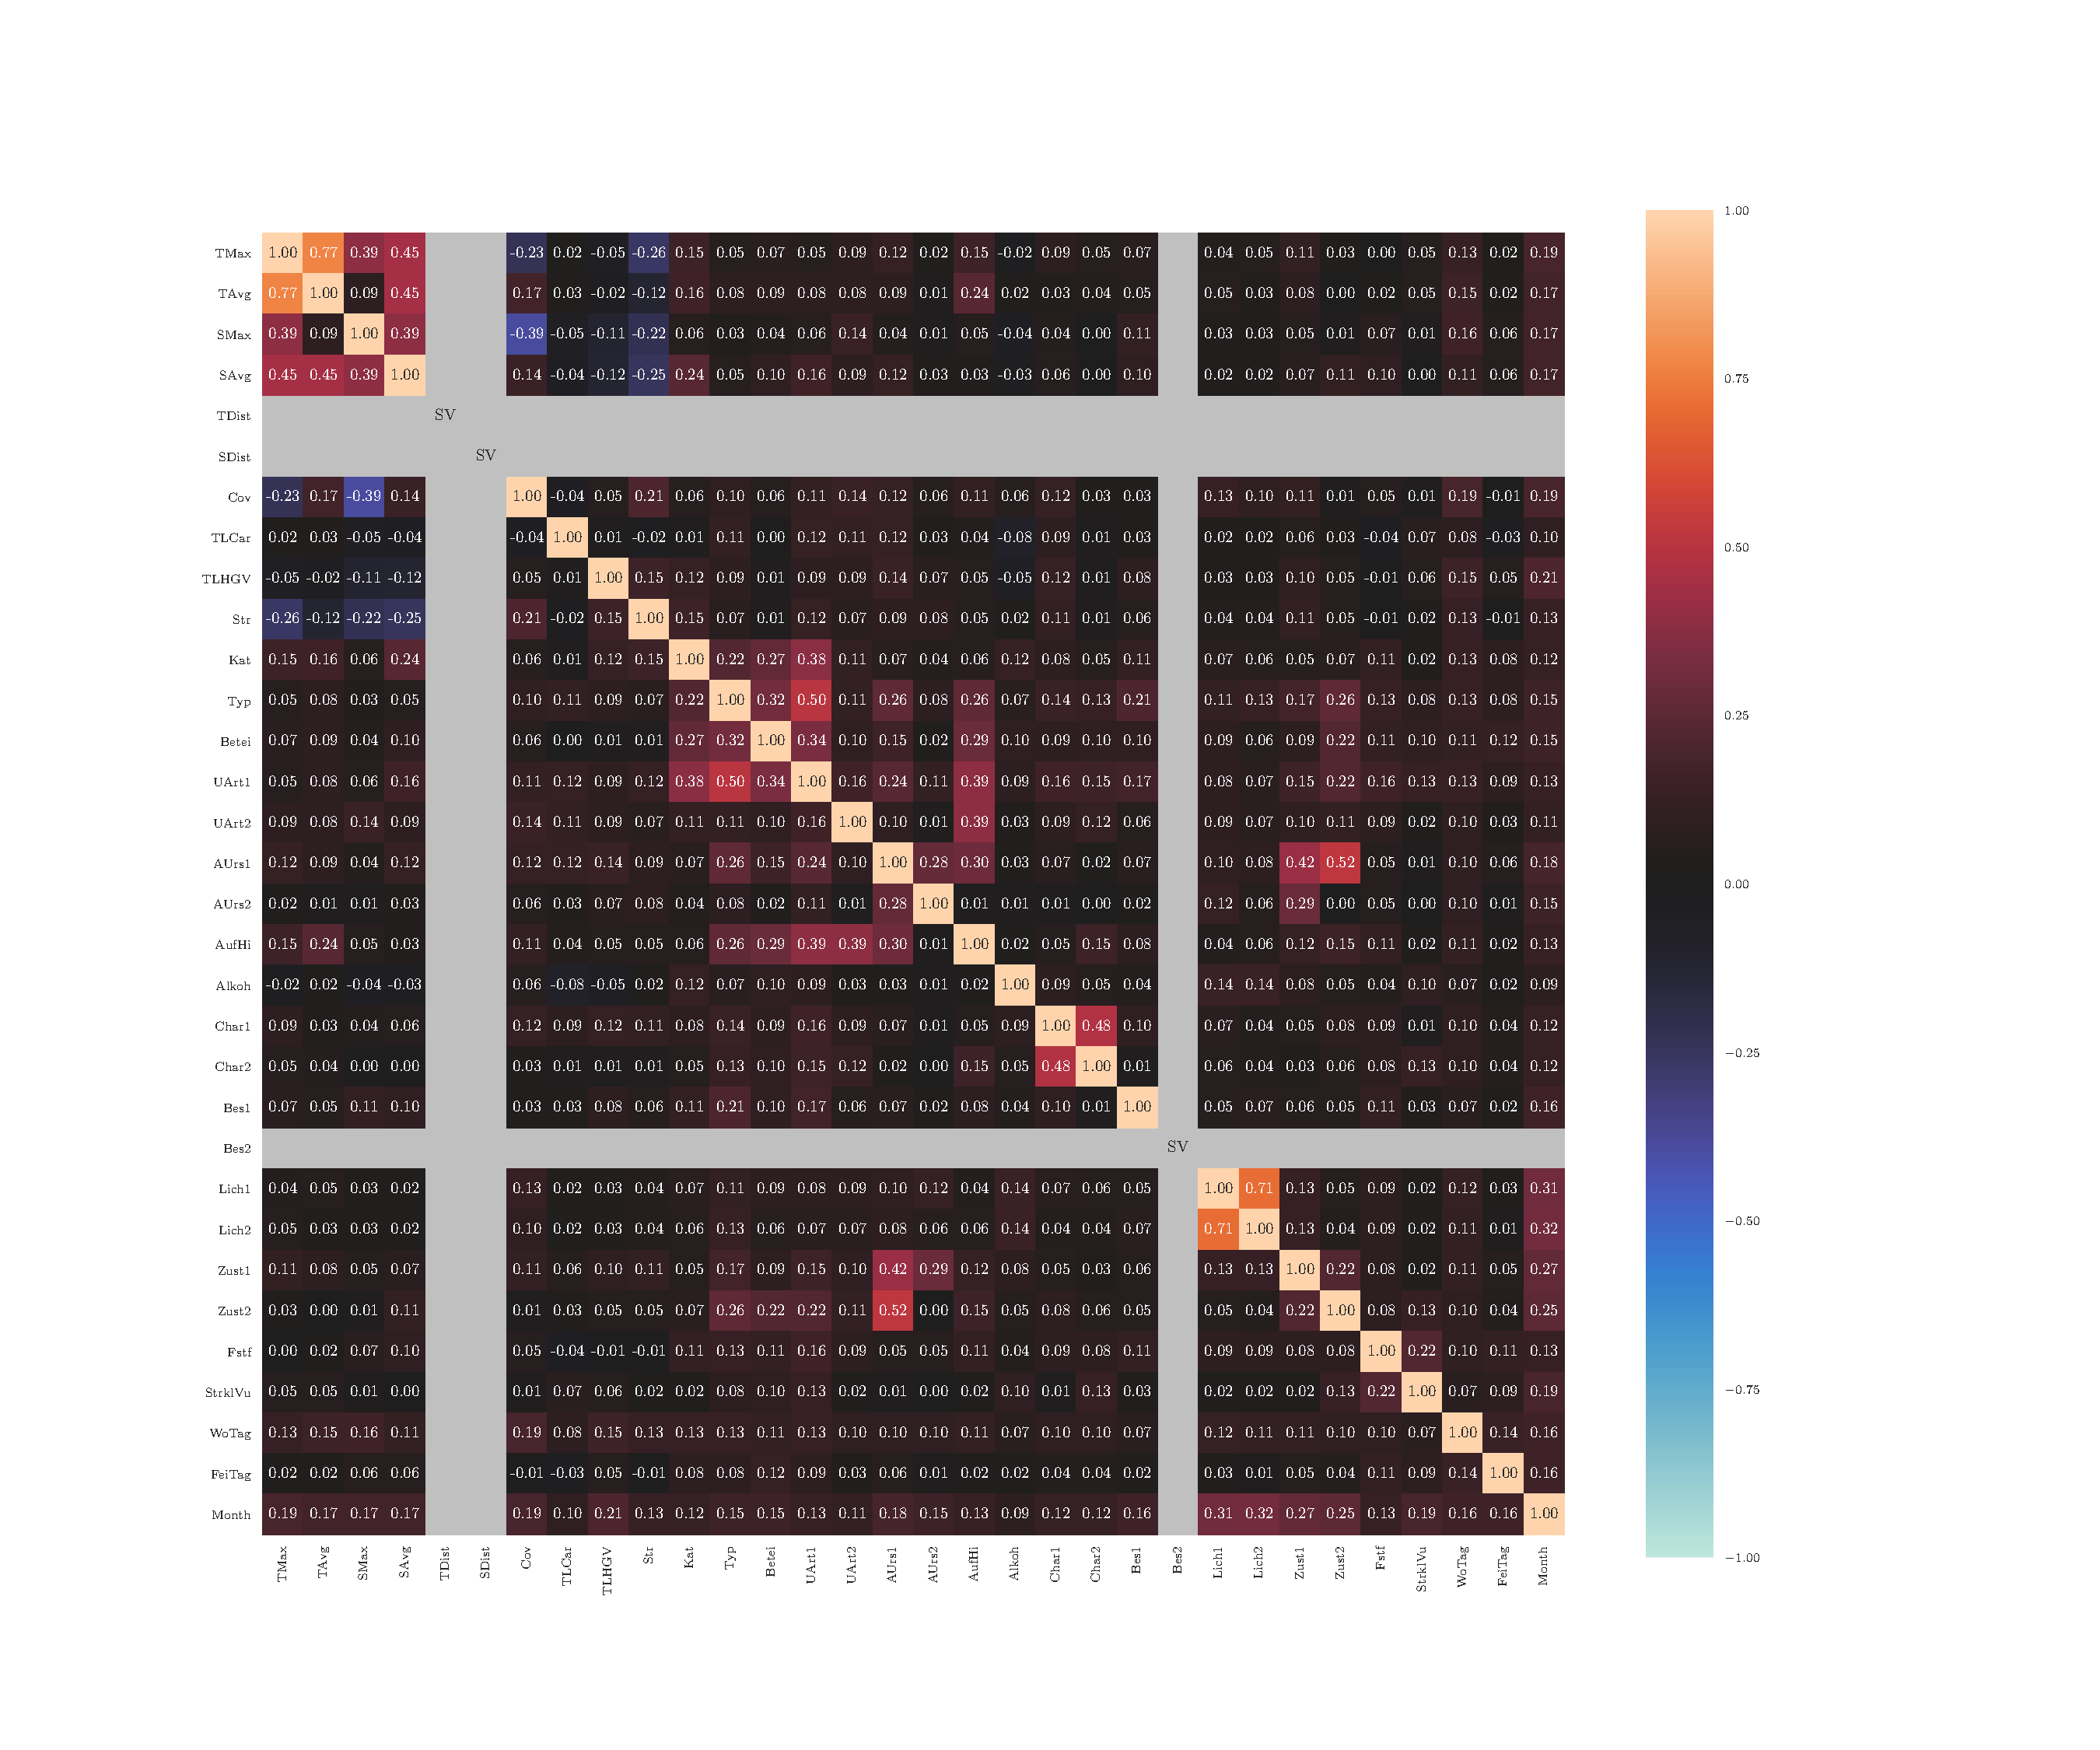
\includegraphics[scale=0.52, trim=2cm 2cm 0cm 0cm]{../CorrAnalysis/data/BAYSIS/03_selected_02_duringJam/plots/baysis_selected_corr_cramers}
    % 	\caption{Correlation matrix for BAYSIS selected data (Jam Effector), with Cramer's $V$}
    % 	\label{img:appendix_correlation_matrix_selected_startJam_cramers}
    % \end{figure}
    % \restoregeometry
    
    % \newgeometry{left=1cm,right=1cm,}
    % \label{appendix_baysis_dataset_corr_theils}
    % \begin{figure}[h]
    % 	\centering
    % 	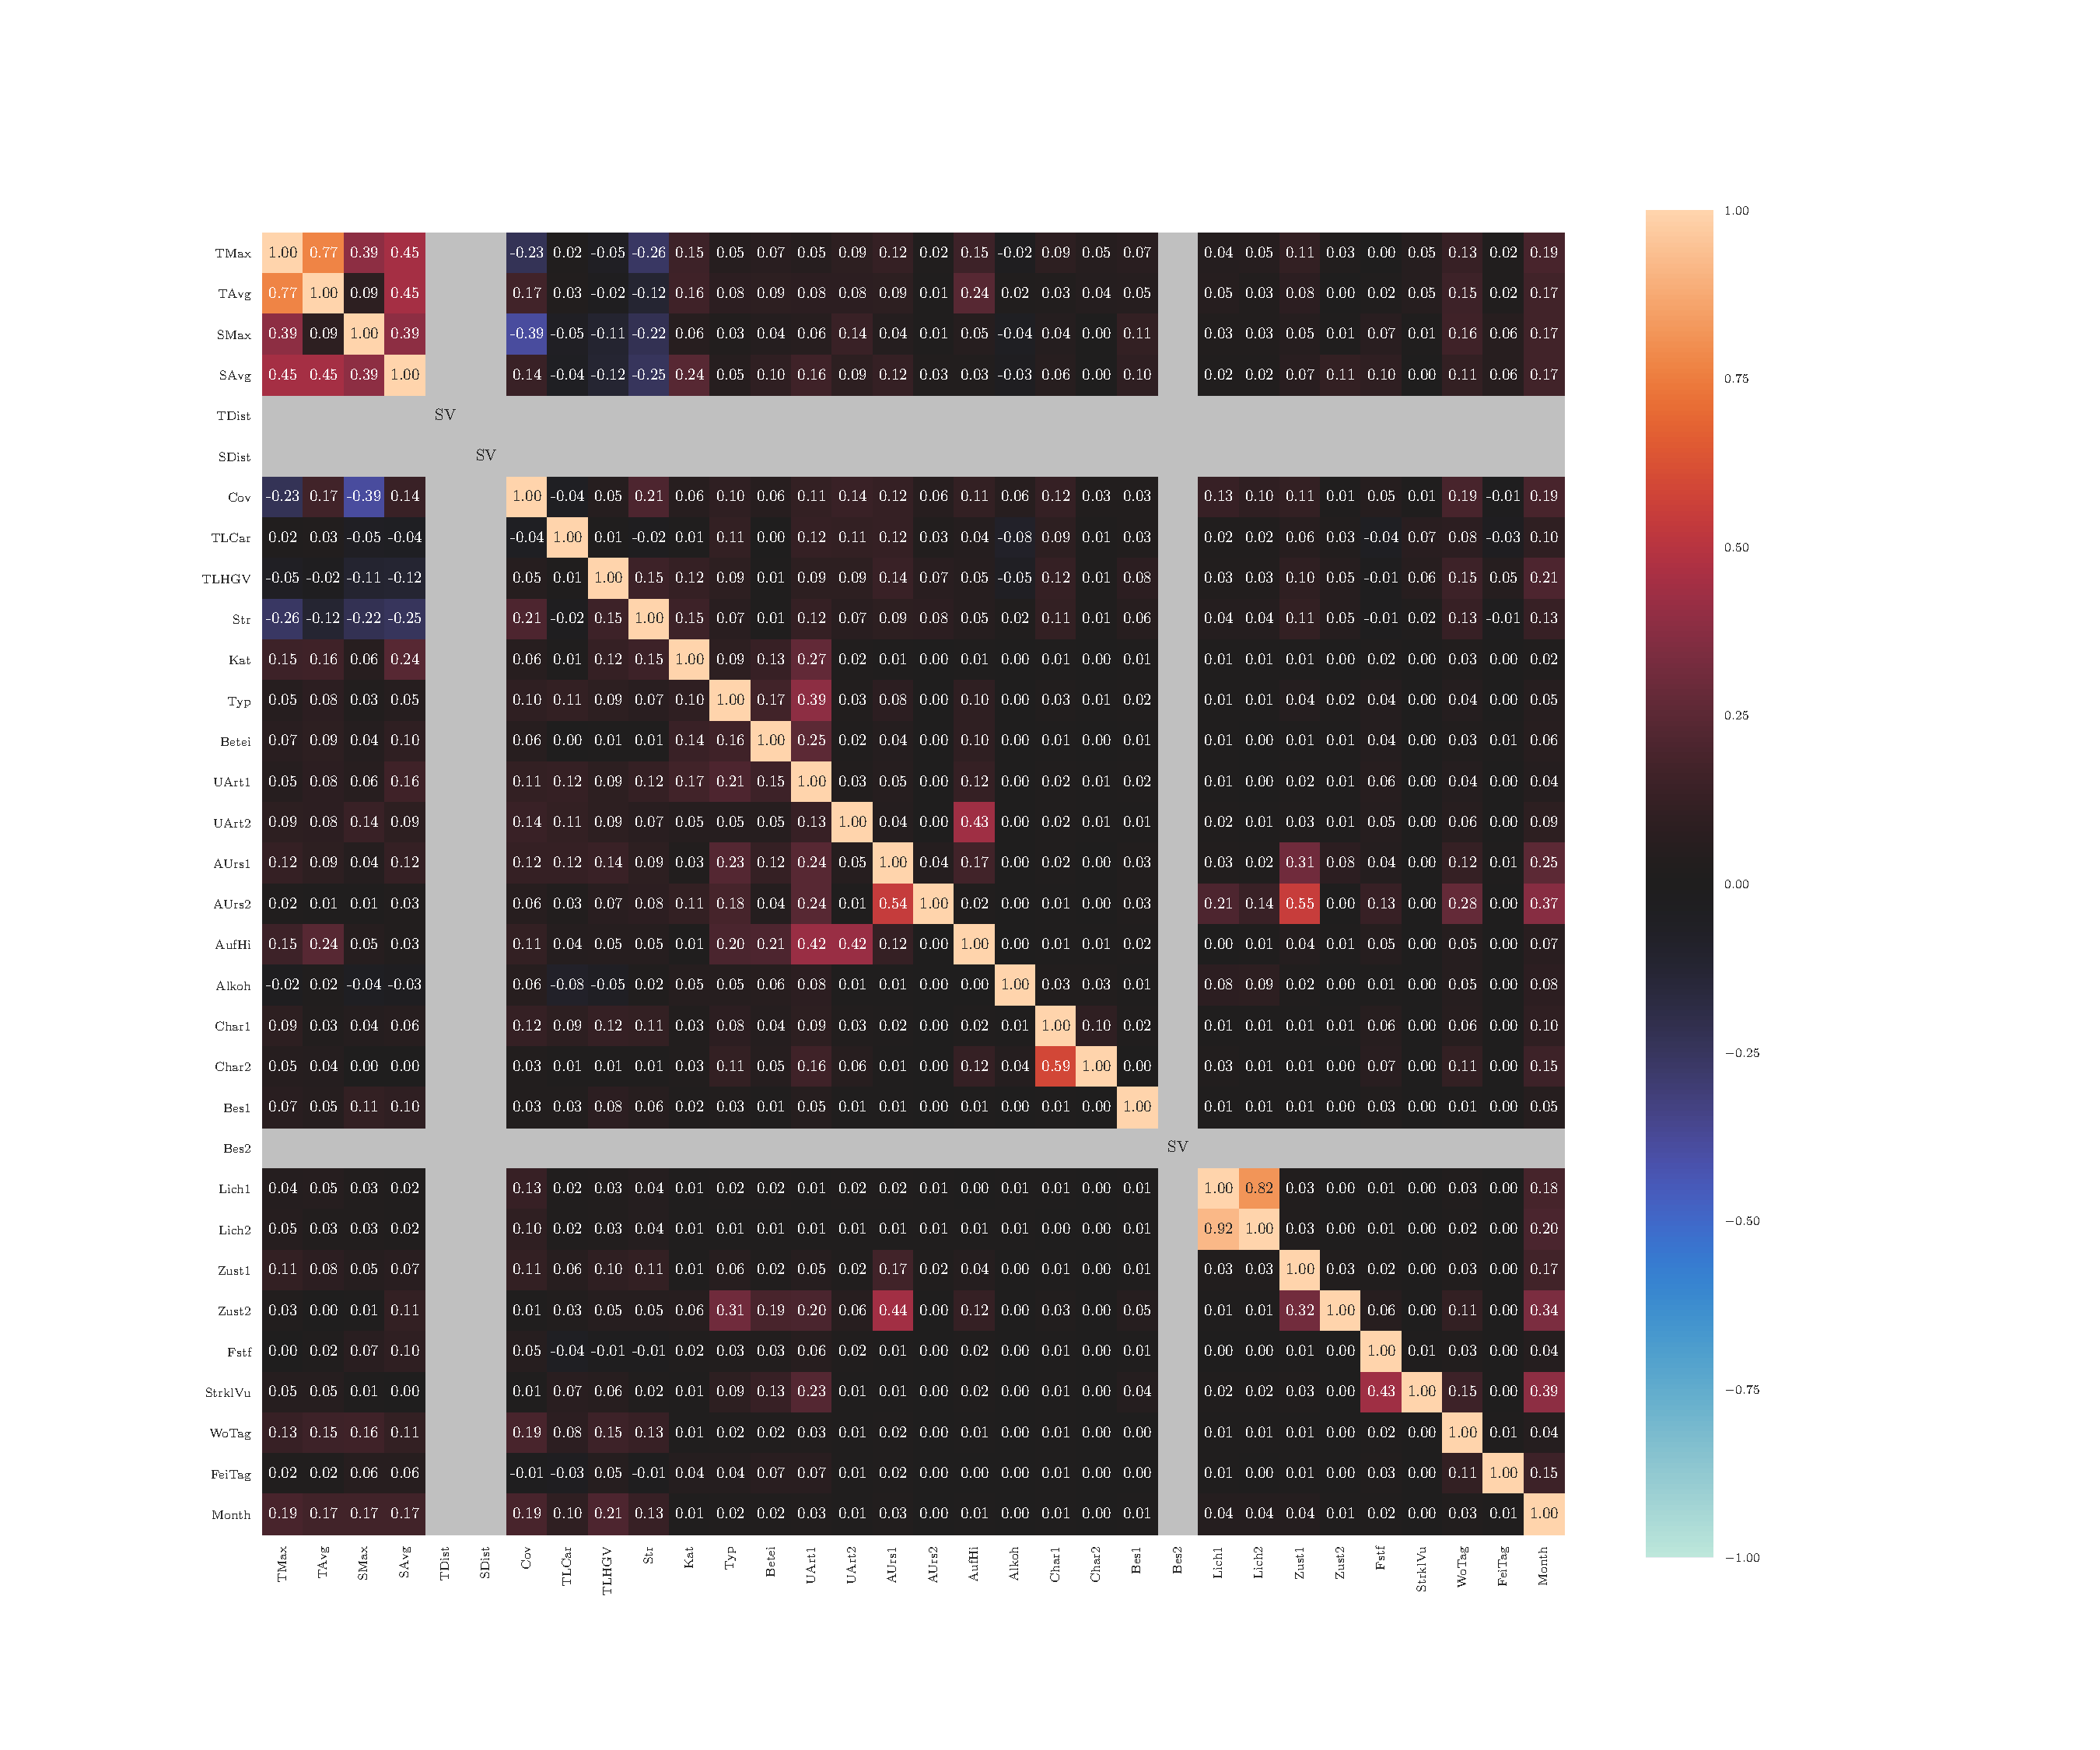
\includegraphics[scale=0.52, trim=2cm 2cm 0cm 0cm]{../CorrAnalysis/data/BAYSIS/03_selected_02_duringJam/plots/baysis_selected_corr_theils}
    % 	\caption{Correlation matrix for BAYSIS selected data (Jam Effector), with Theil's $U$}
    % 	\label{img:appendix_correlation_matrix_selected_startJam_theils}
    % \end{figure}
    % \restoregeometry
    
    % ------- BAYSIS Selected - Tables --------
    \newgeometry{left=1cm,right=1cm,top=1cm}
    \begin{sidewaystable}
    	\tiny
    	\setlength{\tabcolsep}{2pt}
    	\centering
    	\begin{tabular}{lrrrrrrrrrrrrrrrrrrrrrrrrrrrrrrrr}
\toprule
{} &  TMax &  TAvg &  SMax &  SAvg &  TDist &  SDist &   Cov &  TLCar &  TLHGV &   Str &  Kat &  Typ &  Betei &  UArt1 &  UArt2 &  AUrs1 &  AUrs2 &  AufHi &  Alkoh &  Char1 &  Char2 &  Bes1 &  Bes2 &  Lich1 &  Lich2 &  Zust1 &  Zust2 &  Fstf &  StrklVu &  WoTag &  FeiTag &  Month \\
\midrule
TMax    &  1.00 &  0.77 &  0.39 &  0.45 &   0.00 &   0.00 & -0.23 &   0.02 &  -0.05 & -0.26 & 0.15 & 0.05 &   0.07 &   0.05 &   0.09 &   0.12 &   0.02 &   0.15 &  -0.02 &   0.09 &   0.05 &  0.07 &  0.00 &   0.04 &   0.05 &   0.11 &   0.03 &  0.00 &     0.05 &   0.13 &    0.02 &   0.19 \\
TAvg    &  0.77 &  1.00 &  0.09 &  0.45 &   0.00 &   0.00 &  0.17 &   0.03 &  -0.02 & -0.12 & 0.16 & 0.08 &   0.09 &   0.08 &   0.08 &   0.09 &   0.01 &   0.24 &   0.02 &   0.03 &   0.04 &  0.05 &  0.00 &   0.05 &   0.03 &   0.08 &   0.00 &  0.02 &     0.05 &   0.15 &    0.02 &   0.17 \\
SMax    &  0.39 &  0.09 &  1.00 &  0.39 &   0.00 &   0.00 & -0.39 &  -0.05 &  -0.11 & -0.22 & 0.06 & 0.03 &   0.04 &   0.06 &   0.14 &   0.04 &   0.01 &   0.05 &  -0.04 &   0.04 &   0.00 &  0.11 &  0.00 &   0.03 &   0.03 &   0.05 &   0.01 &  0.07 &     0.01 &   0.16 &    0.06 &   0.17 \\
SAvg    &  0.45 &  0.45 &  0.39 &  1.00 &   0.00 &   0.00 &  0.14 &  -0.04 &  -0.12 & -0.25 & 0.24 & 0.05 &   0.10 &   0.16 &   0.09 &   0.12 &   0.03 &   0.03 &  -0.03 &   0.06 &   0.00 &  0.10 &  0.00 &   0.02 &   0.02 &   0.07 &   0.11 &  0.10 &     0.00 &   0.11 &    0.06 &   0.17 \\
TDist   &  0.00 &  0.00 &  0.00 &  0.00 &   0.00 &   0.00 &  0.00 &   0.00 &   0.00 &  0.00 & 0.00 & 0.00 &   0.00 &   0.00 &   0.00 &   0.00 &   0.00 &   0.00 &   0.00 &   0.00 &   0.00 &  0.00 &  0.00 &   0.00 &   0.00 &   0.00 &   0.00 &  0.00 &     0.00 &   0.00 &    0.00 &   0.00 \\
SDist   &  0.00 &  0.00 &  0.00 &  0.00 &   0.00 &   0.00 &  0.00 &   0.00 &   0.00 &  0.00 & 0.00 & 0.00 &   0.00 &   0.00 &   0.00 &   0.00 &   0.00 &   0.00 &   0.00 &   0.00 &   0.00 &  0.00 &  0.00 &   0.00 &   0.00 &   0.00 &   0.00 &  0.00 &     0.00 &   0.00 &    0.00 &   0.00 \\
Cov     & -0.23 &  0.17 & -0.39 &  0.14 &   0.00 &   0.00 &  1.00 &  -0.04 &   0.05 &  0.21 & 0.06 & 0.10 &   0.06 &   0.11 &   0.14 &   0.12 &   0.06 &   0.11 &   0.06 &   0.12 &   0.03 &  0.03 &  0.00 &   0.13 &   0.10 &   0.11 &   0.01 &  0.05 &     0.01 &   0.19 &   -0.01 &   0.19 \\
TLCar   &  0.02 &  0.03 & -0.05 & -0.04 &   0.00 &   0.00 & -0.04 &   1.00 &   0.01 & -0.02 & 0.01 & 0.11 &   0.00 &   0.12 &   0.11 &   0.12 &   0.03 &   0.04 &  -0.08 &   0.09 &   0.01 &  0.03 &  0.00 &   0.02 &   0.02 &   0.06 &   0.03 & -0.04 &     0.07 &   0.08 &   -0.03 &   0.10 \\
TLHGV   & -0.05 & -0.02 & -0.11 & -0.12 &   0.00 &   0.00 &  0.05 &   0.01 &   1.00 &  0.15 & 0.12 & 0.09 &   0.01 &   0.09 &   0.09 &   0.14 &   0.07 &   0.05 &  -0.05 &   0.12 &   0.01 &  0.08 &  0.00 &   0.03 &   0.03 &   0.10 &   0.05 & -0.01 &     0.06 &   0.15 &    0.05 &   0.21 \\
Str     & -0.26 & -0.12 & -0.22 & -0.25 &   0.00 &   0.00 &  0.21 &  -0.02 &   0.15 &  1.00 & 0.15 & 0.07 &   0.01 &   0.12 &   0.07 &   0.09 &   0.08 &   0.05 &   0.02 &   0.11 &   0.01 &  0.06 &  0.00 &   0.04 &   0.04 &   0.11 &   0.05 & -0.01 &     0.02 &   0.13 &   -0.01 &   0.13 \\
Kat     &  0.15 &  0.16 &  0.06 &  0.24 &   0.00 &   0.00 &  0.06 &   0.01 &   0.12 &  0.15 & 1.00 & 0.22 &   0.27 &   0.38 &   0.11 &   0.07 &   0.04 &   0.06 &   0.12 &   0.08 &   0.05 &  0.11 &  0.00 &   0.07 &   0.06 &   0.05 &   0.07 &  0.11 &     0.02 &   0.13 &    0.08 &   0.12 \\
Typ     &  0.05 &  0.08 &  0.03 &  0.05 &   0.00 &   0.00 &  0.10 &   0.11 &   0.09 &  0.07 & 0.22 & 1.00 &   0.32 &   0.50 &   0.11 &   0.26 &   0.08 &   0.26 &   0.07 &   0.14 &   0.13 &  0.21 &  0.00 &   0.11 &   0.13 &   0.17 &   0.26 &  0.13 &     0.08 &   0.13 &    0.08 &   0.15 \\
Betei   &  0.07 &  0.09 &  0.04 &  0.10 &   0.00 &   0.00 &  0.06 &   0.00 &   0.01 &  0.01 & 0.27 & 0.32 &   1.00 &   0.34 &   0.10 &   0.15 &   0.02 &   0.29 &   0.10 &   0.09 &   0.10 &  0.10 &  0.00 &   0.09 &   0.06 &   0.09 &   0.22 &  0.11 &     0.10 &   0.11 &    0.12 &   0.15 \\
UArt1   &  0.05 &  0.08 &  0.06 &  0.16 &   0.00 &   0.00 &  0.11 &   0.12 &   0.09 &  0.12 & 0.38 & 0.50 &   0.34 &   1.00 &   0.16 &   0.24 &   0.11 &   0.39 &   0.09 &   0.16 &   0.15 &  0.17 &  0.00 &   0.08 &   0.07 &   0.15 &   0.22 &  0.16 &     0.13 &   0.13 &    0.09 &   0.13 \\
UArt2   &  0.09 &  0.08 &  0.14 &  0.09 &   0.00 &   0.00 &  0.14 &   0.11 &   0.09 &  0.07 & 0.11 & 0.11 &   0.10 &   0.16 &   1.00 &   0.10 &   0.01 &   0.39 &   0.03 &   0.09 &   0.12 &  0.06 &  0.00 &   0.09 &   0.07 &   0.10 &   0.11 &  0.09 &     0.02 &   0.10 &    0.03 &   0.11 \\
AUrs1   &  0.12 &  0.09 &  0.04 &  0.12 &   0.00 &   0.00 &  0.12 &   0.12 &   0.14 &  0.09 & 0.07 & 0.26 &   0.15 &   0.24 &   0.10 &   1.00 &   0.28 &   0.30 &   0.03 &   0.07 &   0.02 &  0.07 &  0.00 &   0.10 &   0.08 &   0.42 &   0.52 &  0.05 &     0.01 &   0.10 &    0.06 &   0.18 \\
AUrs2   &  0.02 &  0.01 &  0.01 &  0.03 &   0.00 &   0.00 &  0.06 &   0.03 &   0.07 &  0.08 & 0.04 & 0.08 &   0.02 &   0.11 &   0.01 &   0.28 &   1.00 &   0.01 &   0.01 &   0.01 &   0.00 &  0.02 &  0.00 &   0.12 &   0.06 &   0.29 &   0.00 &  0.05 &     0.00 &   0.10 &    0.01 &   0.15 \\
AufHi   &  0.15 &  0.24 &  0.05 &  0.03 &   0.00 &   0.00 &  0.11 &   0.04 &   0.05 &  0.05 & 0.06 & 0.26 &   0.29 &   0.39 &   0.39 &   0.30 &   0.01 &   1.00 &   0.02 &   0.05 &   0.15 &  0.08 &  0.00 &   0.04 &   0.06 &   0.12 &   0.15 &  0.11 &     0.02 &   0.11 &    0.02 &   0.13 \\
Alkoh   & -0.02 &  0.02 & -0.04 & -0.03 &   0.00 &   0.00 &  0.06 &  -0.08 &  -0.05 &  0.02 & 0.12 & 0.07 &   0.10 &   0.09 &   0.03 &   0.03 &   0.01 &   0.02 &   1.00 &   0.09 &   0.05 &  0.04 &  0.00 &   0.14 &   0.14 &   0.08 &   0.05 &  0.04 &     0.10 &   0.07 &    0.02 &   0.09 \\
Char1   &  0.09 &  0.03 &  0.04 &  0.06 &   0.00 &   0.00 &  0.12 &   0.09 &   0.12 &  0.11 & 0.08 & 0.14 &   0.09 &   0.16 &   0.09 &   0.07 &   0.01 &   0.05 &   0.09 &   1.00 &   0.48 &  0.10 &  0.00 &   0.07 &   0.04 &   0.05 &   0.08 &  0.09 &     0.01 &   0.10 &    0.04 &   0.12 \\
Char2   &  0.05 &  0.04 &  0.00 &  0.00 &   0.00 &   0.00 &  0.03 &   0.01 &   0.01 &  0.01 & 0.05 & 0.13 &   0.10 &   0.15 &   0.12 &   0.02 &   0.00 &   0.15 &   0.05 &   0.48 &   1.00 &  0.01 &  0.00 &   0.06 &   0.04 &   0.03 &   0.06 &  0.08 &     0.13 &   0.10 &    0.04 &   0.12 \\
Bes1    &  0.07 &  0.05 &  0.11 &  0.10 &   0.00 &   0.00 &  0.03 &   0.03 &   0.08 &  0.06 & 0.11 & 0.21 &   0.10 &   0.17 &   0.06 &   0.07 &   0.02 &   0.08 &   0.04 &   0.10 &   0.01 &  1.00 &  0.00 &   0.05 &   0.07 &   0.06 &   0.05 &  0.11 &     0.03 &   0.07 &    0.02 &   0.16 \\
Bes2    &  0.00 &  0.00 &  0.00 &  0.00 &   0.00 &   0.00 &  0.00 &   0.00 &   0.00 &  0.00 & 0.00 & 0.00 &   0.00 &   0.00 &   0.00 &   0.00 &   0.00 &   0.00 &   0.00 &   0.00 &   0.00 &  0.00 &  0.00 &   0.00 &   0.00 &   0.00 &   0.00 &  0.00 &     0.00 &   0.00 &    0.00 &   0.00 \\
Lich1   &  0.04 &  0.05 &  0.03 &  0.02 &   0.00 &   0.00 &  0.13 &   0.02 &   0.03 &  0.04 & 0.07 & 0.11 &   0.09 &   0.08 &   0.09 &   0.10 &   0.12 &   0.04 &   0.14 &   0.07 &   0.06 &  0.05 &  0.00 &   1.00 &   0.71 &   0.13 &   0.05 &  0.09 &     0.02 &   0.12 &    0.03 &   0.31 \\
Lich2   &  0.05 &  0.03 &  0.03 &  0.02 &   0.00 &   0.00 &  0.10 &   0.02 &   0.03 &  0.04 & 0.06 & 0.13 &   0.06 &   0.07 &   0.07 &   0.08 &   0.06 &   0.06 &   0.14 &   0.04 &   0.04 &  0.07 &  0.00 &   0.71 &   1.00 &   0.13 &   0.04 &  0.09 &     0.02 &   0.11 &    0.01 &   0.32 \\
Zust1   &  0.11 &  0.08 &  0.05 &  0.07 &   0.00 &   0.00 &  0.11 &   0.06 &   0.10 &  0.11 & 0.05 & 0.17 &   0.09 &   0.15 &   0.10 &   0.42 &   0.29 &   0.12 &   0.08 &   0.05 &   0.03 &  0.06 &  0.00 &   0.13 &   0.13 &   1.00 &   0.22 &  0.08 &     0.02 &   0.11 &    0.05 &   0.27 \\
Zust2   &  0.03 &  0.00 &  0.01 &  0.11 &   0.00 &   0.00 &  0.01 &   0.03 &   0.05 &  0.05 & 0.07 & 0.26 &   0.22 &   0.22 &   0.11 &   0.52 &   0.00 &   0.15 &   0.05 &   0.08 &   0.06 &  0.05 &  0.00 &   0.05 &   0.04 &   0.22 &   1.00 &  0.08 &     0.13 &   0.10 &    0.04 &   0.25 \\
Fstf    &  0.00 &  0.02 &  0.07 &  0.10 &   0.00 &   0.00 &  0.05 &  -0.04 &  -0.01 & -0.01 & 0.11 & 0.13 &   0.11 &   0.16 &   0.09 &   0.05 &   0.05 &   0.11 &   0.04 &   0.09 &   0.08 &  0.11 &  0.00 &   0.09 &   0.09 &   0.08 &   0.08 &  1.00 &     0.22 &   0.10 &    0.11 &   0.13 \\
StrklVu &  0.05 &  0.05 &  0.01 &  0.00 &   0.00 &   0.00 &  0.01 &   0.07 &   0.06 &  0.02 & 0.02 & 0.08 &   0.10 &   0.13 &   0.02 &   0.01 &   0.00 &   0.02 &   0.10 &   0.01 &   0.13 &  0.03 &  0.00 &   0.02 &   0.02 &   0.02 &   0.13 &  0.22 &     1.00 &   0.07 &    0.09 &   0.19 \\
WoTag   &  0.13 &  0.15 &  0.16 &  0.11 &   0.00 &   0.00 &  0.19 &   0.08 &   0.15 &  0.13 & 0.13 & 0.13 &   0.11 &   0.13 &   0.10 &   0.10 &   0.10 &   0.11 &   0.07 &   0.10 &   0.10 &  0.07 &  0.00 &   0.12 &   0.11 &   0.11 &   0.10 &  0.10 &     0.07 &   1.00 &    0.14 &   0.16 \\
FeiTag  &  0.02 &  0.02 &  0.06 &  0.06 &   0.00 &   0.00 & -0.01 &  -0.03 &   0.05 & -0.01 & 0.08 & 0.08 &   0.12 &   0.09 &   0.03 &   0.06 &   0.01 &   0.02 &   0.02 &   0.04 &   0.04 &  0.02 &  0.00 &   0.03 &   0.01 &   0.05 &   0.04 &  0.11 &     0.09 &   0.14 &    1.00 &   0.16 \\
Month   &  0.19 &  0.17 &  0.17 &  0.17 &   0.00 &   0.00 &  0.19 &   0.10 &   0.21 &  0.13 & 0.12 & 0.15 &   0.15 &   0.13 &   0.11 &   0.18 &   0.15 &   0.13 &   0.09 &   0.12 &   0.12 &  0.16 &  0.00 &   0.31 &   0.32 &   0.27 &   0.25 &  0.13 &     0.19 &   0.16 &    0.16 &   1.00 \\
\bottomrule
\end{tabular}

    	\caption{Correlation matrix for BAYSIS selected data (Jam Effector), with Cramer's $V$}
    	\label{table:appendix_correlation_matrix_selected_startJam_cramers}
    \end{sidewaystable}
    
    \newgeometry{left=1cm,right=1cm,top=1cm}
    \begin{sidewaystable}
    	\tiny
    	\setlength{\tabcolsep}{2pt}
    	\centering
    	\begin{tabular}{lrrrrrrrrrrrrrrrrrrrrrrrrrrrrr}
\toprule
{} &  TMax &  TAvg &  SMax &  SAvg &  TDist &  SDist &   Cov &  TLCar &  TLHGV &  Str &  Kat &  Typ &  Betei &  UArt1 &  UArt2 &  AUrs1 &  AUrs2 &  AufHi &  Alkoh &  Char1 &  Char2 &  Lich1 &  Lich2 &  Zust1 &  Zust2 &  Fstf &  WoTag &  FeiTag &  Month \\
\midrule
TMax   &  1.00 &  0.77 &  0.39 &  0.45 &   0.00 &   0.00 & -0.23 &   0.02 &  -0.05 & 0.29 & 0.15 & 0.05 &   0.07 &   0.05 &   0.09 &   0.12 &   0.02 &   0.15 &  -0.02 &   0.09 &   0.05 &   0.04 &   0.05 &   0.11 &   0.03 &  0.00 &   0.13 &    0.02 &   0.19 \\
TAvg   &  0.77 &  1.00 &  0.09 &  0.45 &   0.00 &   0.00 &  0.17 &   0.03 &  -0.02 & 0.24 & 0.16 & 0.08 &   0.09 &   0.08 &   0.08 &   0.09 &   0.01 &   0.24 &   0.02 &   0.03 &   0.04 &   0.05 &   0.03 &   0.08 &   0.00 &  0.02 &   0.15 &    0.02 &   0.17 \\
SMax   &  0.39 &  0.09 &  1.00 &  0.39 &   0.00 &   0.00 & -0.39 &  -0.05 &  -0.11 & 0.27 & 0.06 & 0.03 &   0.04 &   0.06 &   0.14 &   0.04 &   0.01 &   0.05 &  -0.04 &   0.04 &   0.00 &   0.03 &   0.03 &   0.05 &   0.01 &  0.07 &   0.16 &    0.06 &   0.17 \\
SAvg   &  0.45 &  0.45 &  0.39 &  1.00 &   0.00 &   0.00 &  0.14 &  -0.04 &  -0.12 & 0.32 & 0.24 & 0.05 &   0.10 &   0.16 &   0.09 &   0.12 &   0.03 &   0.03 &  -0.03 &   0.06 &   0.00 &   0.02 &   0.02 &   0.07 &   0.11 &  0.10 &   0.11 &    0.06 &   0.17 \\
TDist  &  0.00 &  0.00 &  0.00 &  0.00 &   0.00 &   0.00 &  0.00 &   0.00 &   0.00 & 0.00 & 0.00 & 0.00 &   0.00 &   0.00 &   0.00 &   0.00 &   0.00 &   0.00 &   0.00 &   0.00 &   0.00 &   0.00 &   0.00 &   0.00 &   0.00 &  0.00 &   0.00 &    0.00 &   0.00 \\
SDist  &  0.00 &  0.00 &  0.00 &  0.00 &   0.00 &   0.00 &  0.00 &   0.00 &   0.00 & 0.00 & 0.00 & 0.00 &   0.00 &   0.00 &   0.00 &   0.00 &   0.00 &   0.00 &   0.00 &   0.00 &   0.00 &   0.00 &   0.00 &   0.00 &   0.00 &  0.00 &   0.00 &    0.00 &   0.00 \\
Cov    & -0.23 &  0.17 & -0.39 &  0.14 &   0.00 &   0.00 &  1.00 &  -0.04 &   0.05 & 0.32 & 0.06 & 0.10 &   0.06 &   0.11 &   0.14 &   0.12 &   0.06 &   0.11 &   0.06 &   0.12 &   0.03 &   0.13 &   0.10 &   0.11 &   0.01 &  0.05 &   0.19 &   -0.01 &   0.19 \\
TLCar  &  0.02 &  0.03 & -0.05 & -0.04 &   0.00 &   0.00 & -0.04 &   1.00 &   0.01 & 0.12 & 0.01 & 0.11 &   0.00 &   0.12 &   0.11 &   0.12 &   0.03 &   0.04 &  -0.08 &   0.09 &   0.01 &   0.02 &   0.02 &   0.06 &   0.03 & -0.04 &   0.08 &   -0.03 &   0.10 \\
TLHGV  & -0.05 & -0.02 & -0.11 & -0.12 &   0.00 &   0.00 &  0.05 &   0.01 &   1.00 & 0.21 & 0.12 & 0.09 &   0.01 &   0.09 &   0.09 &   0.14 &   0.07 &   0.05 &  -0.05 &   0.12 &   0.01 &   0.03 &   0.03 &   0.10 &   0.05 & -0.01 &   0.15 &    0.05 &   0.21 \\
Str    &  0.29 &  0.24 &  0.27 &  0.32 &   0.00 &   0.00 &  0.32 &   0.12 &   0.21 & 1.00 & 0.02 & 0.02 &   0.02 &   0.04 &   0.02 &   0.02 &   0.00 &   0.01 &   0.00 &   0.02 &   0.00 &   0.01 &   0.01 &   0.01 &   0.00 &  0.05 &   0.05 &    0.00 &   0.06 \\
Kat    &  0.15 &  0.16 &  0.06 &  0.24 &   0.00 &   0.00 &  0.06 &   0.01 &   0.12 & 0.03 & 1.00 & 0.09 &   0.13 &   0.27 &   0.02 &   0.01 &   0.00 &   0.01 &   0.00 &   0.01 &   0.00 &   0.01 &   0.01 &   0.01 &   0.00 &  0.02 &   0.03 &    0.00 &   0.02 \\
Typ    &  0.05 &  0.08 &  0.03 &  0.05 &   0.00 &   0.00 &  0.10 &   0.11 &   0.09 & 0.05 & 0.10 & 1.00 &   0.17 &   0.39 &   0.03 &   0.08 &   0.00 &   0.10 &   0.00 &   0.03 &   0.01 &   0.01 &   0.01 &   0.04 &   0.02 &  0.04 &   0.04 &    0.00 &   0.05 \\
Betei  &  0.07 &  0.09 &  0.04 &  0.10 &   0.00 &   0.00 &  0.06 &   0.00 &   0.01 & 0.04 & 0.14 & 0.16 &   1.00 &   0.25 &   0.02 &   0.04 &   0.00 &   0.10 &   0.00 &   0.01 &   0.00 &   0.01 &   0.00 &   0.01 &   0.01 &  0.04 &   0.03 &    0.01 &   0.06 \\
UArt1  &  0.05 &  0.08 &  0.06 &  0.16 &   0.00 &   0.00 &  0.11 &   0.12 &   0.09 & 0.05 & 0.17 & 0.21 &   0.15 &   1.00 &   0.03 &   0.05 &   0.00 &   0.12 &   0.00 &   0.02 &   0.01 &   0.01 &   0.00 &   0.02 &   0.01 &  0.06 &   0.04 &    0.00 &   0.04 \\
UArt2  &  0.09 &  0.08 &  0.14 &  0.09 &   0.00 &   0.00 &  0.14 &   0.11 &   0.09 & 0.10 & 0.05 & 0.05 &   0.05 &   0.13 &   1.00 &   0.04 &   0.00 &   0.43 &   0.00 &   0.02 &   0.01 &   0.02 &   0.01 &   0.03 &   0.01 &  0.05 &   0.06 &    0.00 &   0.09 \\
AUrs1  &  0.12 &  0.09 &  0.04 &  0.12 &   0.00 &   0.00 &  0.12 &   0.12 &   0.14 & 0.11 & 0.03 & 0.23 &   0.12 &   0.24 &   0.05 &   1.00 &   0.04 &   0.17 &   0.00 &   0.02 &   0.00 &   0.03 &   0.02 &   0.31 &   0.08 &  0.04 &   0.12 &    0.01 &   0.25 \\
AUrs2  &  0.02 &  0.01 &  0.01 &  0.03 &   0.00 &   0.00 &  0.06 &   0.03 &   0.07 & 0.26 & 0.11 & 0.18 &   0.04 &   0.24 &   0.01 &   0.54 &   1.00 &   0.02 &   0.00 &   0.01 &   0.00 &   0.21 &   0.14 &   0.55 &   0.00 &  0.13 &   0.28 &    0.00 &   0.37 \\
AufHi  &  0.15 &  0.24 &  0.05 &  0.03 &   0.00 &   0.00 &  0.11 &   0.04 &   0.05 & 0.06 & 0.01 & 0.20 &   0.21 &   0.42 &   0.42 &   0.12 &   0.00 &   1.00 &   0.00 &   0.01 &   0.01 &   0.00 &   0.01 &   0.04 &   0.01 &  0.05 &   0.05 &    0.00 &   0.07 \\
Alkoh  & -0.02 &  0.02 & -0.04 & -0.03 &   0.00 &   0.00 &  0.06 &  -0.08 &  -0.05 & 0.04 & 0.05 & 0.05 &   0.06 &   0.08 &   0.01 &   0.01 &   0.00 &   0.00 &   1.00 &   0.03 &   0.03 &   0.08 &   0.09 &   0.02 &   0.00 &  0.01 &   0.05 &    0.00 &   0.08 \\
Char1  &  0.09 &  0.03 &  0.04 &  0.06 &   0.00 &   0.00 &  0.12 &   0.09 &   0.12 & 0.14 & 0.03 & 0.08 &   0.04 &   0.09 &   0.03 &   0.02 &   0.00 &   0.02 &   0.01 &   1.00 &   0.10 &   0.01 &   0.01 &   0.01 &   0.01 &  0.06 &   0.06 &    0.00 &   0.10 \\
Char2  &  0.05 &  0.04 &  0.00 &  0.00 &   0.00 &   0.00 &  0.03 &   0.01 &   0.01 & 0.12 & 0.03 & 0.11 &   0.05 &   0.16 &   0.06 &   0.01 &   0.00 &   0.12 &   0.04 &   0.59 &   1.00 &   0.03 &   0.01 &   0.01 &   0.00 &  0.07 &   0.11 &    0.00 &   0.15 \\
Lich1  &  0.04 &  0.05 &  0.03 &  0.02 &   0.00 &   0.00 &  0.13 &   0.02 &   0.03 & 0.05 & 0.01 & 0.02 &   0.02 &   0.01 &   0.02 &   0.02 &   0.01 &   0.00 &   0.01 &   0.01 &   0.00 &   1.00 &   0.82 &   0.03 &   0.00 &  0.01 &   0.03 &    0.00 &   0.18 \\
Lich2  &  0.05 &  0.03 &  0.03 &  0.02 &   0.00 &   0.00 &  0.10 &   0.02 &   0.03 & 0.05 & 0.01 & 0.01 &   0.01 &   0.01 &   0.01 &   0.01 &   0.01 &   0.01 &   0.01 &   0.00 &   0.00 &   0.92 &   1.00 &   0.03 &   0.00 &  0.01 &   0.02 &    0.00 &   0.20 \\
Zust1  &  0.11 &  0.08 &  0.05 &  0.07 &   0.00 &   0.00 &  0.11 &   0.06 &   0.10 & 0.05 & 0.01 & 0.06 &   0.02 &   0.05 &   0.02 &   0.17 &   0.02 &   0.04 &   0.00 &   0.01 &   0.00 &   0.03 &   0.03 &   1.00 &   0.03 &  0.02 &   0.03 &    0.00 &   0.17 \\
Zust2  &  0.03 &  0.00 &  0.01 &  0.11 &   0.00 &   0.00 &  0.01 &   0.03 &   0.05 & 0.16 & 0.06 & 0.31 &   0.19 &   0.20 &   0.06 &   0.44 &   0.00 &   0.12 &   0.00 &   0.03 &   0.00 &   0.01 &   0.01 &   0.32 &   1.00 &  0.06 &   0.11 &    0.00 &   0.34 \\
Fstf   &  0.00 &  0.02 &  0.07 &  0.10 &   0.00 &   0.00 &  0.05 &  -0.04 &  -0.01 & 0.07 & 0.02 & 0.03 &   0.03 &   0.06 &   0.02 &   0.01 &   0.00 &   0.02 &   0.00 &   0.01 &   0.00 &   0.00 &   0.00 &   0.01 &   0.00 &  1.00 &   0.03 &    0.00 &   0.04 \\
WoTag  &  0.13 &  0.15 &  0.16 &  0.11 &   0.00 &   0.00 &  0.19 &   0.08 &   0.15 & 0.05 & 0.01 & 0.02 &   0.02 &   0.03 &   0.01 &   0.02 &   0.00 &   0.01 &   0.00 &   0.01 &   0.00 &   0.01 &   0.01 &   0.01 &   0.00 &  0.02 &   1.00 &    0.01 &   0.04 \\
FeiTag &  0.02 &  0.02 &  0.06 &  0.06 &   0.00 &   0.00 & -0.01 &  -0.03 &   0.05 & 0.09 & 0.04 & 0.04 &   0.07 &   0.07 &   0.01 &   0.02 &   0.00 &   0.00 &   0.00 &   0.01 &   0.00 &   0.01 &   0.00 &   0.01 &   0.00 &  0.03 &   0.11 &    1.00 &   0.15 \\
Month  &  0.19 &  0.17 &  0.17 &  0.17 &   0.00 &   0.00 &  0.19 &   0.10 &   0.21 & 0.04 & 0.01 & 0.02 &   0.02 &   0.03 &   0.01 &   0.03 &   0.00 &   0.01 &   0.00 &   0.01 &   0.00 &   0.04 &   0.04 &   0.04 &   0.01 &  0.02 &   0.03 &    0.01 &   1.00 \\
\bottomrule
\end{tabular}

    	\caption{Correlation matrix for BAYSIS selected data (Jam Effector), with Theil's $U$}
    	\label{table:appendix_correlation_matrix_selected_startJam_cramers}
    \end{sidewaystable}
    
    \newgeometry{left=1cm,right=1cm,top=1cm}
    \begin{sidewaystable}
    	\tiny
    	\setlength{\tabcolsep}{2pt}
    	\centering
    	\begin{tabular}{lrrrrrrrrrrrrrrrrrrrrrrrrrrrrrrr}
\toprule
{} &  TMax &  TAvg &  SMax &  SAvg &  TDist &  SDist &   Cov &  TLCar &  TLHGV &   Str &   Kat &   Typ &  Betei &  UArt1 &  UArt2 &  AUrs1 &  AUrs2 &  AufHi &  Alkoh &  Char1 &  Char2 &  Bes1 &  Bes2 &  Lich1 &  Lich2 &  Zust1 &  Zust2 &  Fstf &  WoTag &  FeiTag &  Month \\
\midrule
TMax   &   nan & 0.000 & 0.000 & 0.000 &    nan &    nan & 0.000 &  0.538 &  0.185 & 0.000 & 0.000 & 0.000 &  0.015 &  0.000 &  0.000 &  0.000 &  0.000 &  0.000 &  0.521 &  0.000 &  0.000 & 0.000 &   nan &  0.000 &  0.000 &  0.000 &  0.000 & 0.880 &  0.000 &   0.404 &  0.000 \\
TAvg   & 0.000 &   nan & 0.016 & 0.000 &    nan &    nan & 0.000 &  0.469 &  0.525 & 0.000 & 0.000 & 0.000 &  0.002 &  0.000 &  0.000 &  0.000 &  0.000 &  0.000 &  0.593 &  0.000 &  0.000 & 0.000 &   nan &  0.000 &  0.000 &  0.000 &  0.000 & 0.472 &  0.000 &   0.597 &  0.000 \\
SMax   & 0.000 & 0.016 &   nan & 0.000 &    nan &    nan & 0.000 &  0.172 &  0.003 & 0.000 & 0.000 & 0.000 &  0.119 &  0.000 &  0.000 &  0.000 &  0.000 &  0.000 &  0.335 &  0.000 &  0.000 & 0.000 &   nan &  0.000 &  0.000 &  0.000 &  0.000 & 0.014 &  0.000 &   0.043 &  0.000 \\
SAvg   & 0.000 & 0.000 & 0.000 &   nan &    nan &    nan & 0.000 &  0.307 &  0.001 & 0.000 & 0.000 & 0.000 &  0.001 &  0.000 &  0.000 &  0.000 &  0.000 &  0.000 &  0.390 &  0.000 &  0.000 & 0.000 &   nan &  0.000 &  0.000 &  0.000 &  0.000 & 0.001 &  0.000 &   0.030 &  0.000 \\
TDist  &   nan &   nan &   nan &   nan &    nan &    nan &   nan &    nan &    nan &   nan &   nan &   nan &    nan &    nan &    nan &    nan &    nan &    nan &    nan &    nan &    nan &   nan &   nan &    nan &    nan &    nan &    nan &   nan &    nan &     nan &    nan \\
SDist  &   nan &   nan &   nan &   nan &    nan &    nan &   nan &    nan &    nan &   nan &   nan &   nan &    nan &    nan &    nan &    nan &    nan &    nan &    nan &    nan &    nan &   nan &   nan &    nan &    nan &    nan &    nan &   nan &    nan &     nan &    nan \\
Cov    & 0.000 & 0.000 & 0.000 & 0.000 &    nan &    nan &   nan &  0.308 &  0.135 & 0.000 & 0.000 & 0.000 &  0.047 &  0.000 &  0.000 &  0.000 &  0.000 &  0.000 &  0.117 &  0.000 &  0.000 & 0.000 &   nan &  0.000 &  0.000 &  0.000 &  0.000 & 0.066 &  0.000 &   0.867 &  0.000 \\
TLCar  & 0.538 & 0.469 & 0.172 & 0.307 &    nan &    nan & 0.308 &    nan &  0.818 & 0.000 & 0.000 & 0.000 &  0.981 &  0.000 &  0.000 &  0.000 &  0.000 &  0.000 &  0.029 &  0.000 &  0.000 & 0.000 &   nan &  0.000 &  0.000 &  0.000 &  0.000 & 0.105 &  0.000 &   0.245 &  0.000 \\
TLHGV  & 0.185 & 0.525 & 0.003 & 0.001 &    nan &    nan & 0.135 &  0.818 &    nan & 0.000 & 0.000 & 0.000 &  0.754 &  0.000 &  0.000 &  0.000 &  0.000 &  0.000 &  0.211 &  0.000 &  0.000 & 0.000 &   nan &  0.000 &  0.000 &  0.000 &  0.000 & 0.706 &  0.000 &   0.109 &  0.000 \\
Str    & 0.000 & 0.000 & 0.000 & 0.000 &    nan &    nan & 0.000 &  0.000 &  0.000 &   nan & 0.291 & 0.105 &  0.786 &  0.000 &  0.133 &  0.138 &  0.830 &  0.831 &  0.987 &  0.000 &  0.188 & 0.000 &   nan &  0.005 &  0.042 &  0.000 &  0.353 & 0.000 &  0.000 &   0.637 &  0.025 \\
Kat    & 0.000 & 0.000 & 0.000 & 0.000 &    nan &    nan & 0.000 &  0.000 &  0.000 & 0.291 &   nan & 0.000 &  0.000 &  0.000 &  0.055 &  0.935 &  0.848 &  0.846 &  0.011 &  0.234 &  0.668 & 0.005 &   nan &  0.283 &  0.456 &  0.802 &  0.290 & 0.200 &  0.020 &   0.163 &  0.475 \\
Typ    & 0.000 & 0.000 & 0.000 & 0.000 &    nan &    nan & 0.000 &  0.000 &  0.000 & 0.105 & 0.000 &   nan &  0.000 &  0.000 &  0.094 &  0.000 &  0.226 &  0.000 &  0.483 &  0.000 &  0.012 & 0.000 &   nan &  0.011 &  0.003 &  0.000 &  0.000 & 0.002 &  0.011 &   0.324 &  0.028 \\
Betei  & 0.015 & 0.002 & 0.119 & 0.001 &    nan &    nan & 0.047 &  0.981 &  0.754 & 0.786 & 0.000 & 0.000 &    nan &  0.000 &  0.150 &  0.000 &  1.000 &  0.000 &  0.263 &  0.514 &  0.309 & 0.272 &   nan &  0.341 &  0.927 &  0.320 &  0.000 & 0.064 &  0.037 &   0.077 &  0.005 \\
UArt1  & 0.000 & 0.000 & 0.000 & 0.000 &    nan &    nan & 0.000 &  0.000 &  0.000 & 0.000 & 0.000 & 0.000 &  0.000 &    nan &  0.000 &  0.000 &  0.342 &  0.000 &  0.580 &  0.000 &  0.029 & 0.000 &   nan &  0.856 &  0.970 &  0.001 &  0.000 & 0.000 &  0.004 &   0.568 &  0.243 \\
UArt2  & 0.000 & 0.000 & 0.000 & 0.000 &    nan &    nan & 0.000 &  0.000 &  0.000 & 0.133 & 0.055 & 0.094 &  0.150 &  0.000 &    nan &  0.216 &  1.000 &  0.000 &  0.993 &  0.479 &  0.100 & 0.901 &   nan &  0.468 &  0.885 &  0.170 &  0.214 & 0.580 &  0.283 &   0.995 &  0.819 \\
AUrs1  & 0.000 & 0.000 & 0.000 & 0.000 &    nan &    nan & 0.000 &  0.000 &  0.000 & 0.138 & 0.935 & 0.000 &  0.000 &  0.000 &  0.216 &    nan &  0.000 &  0.000 &  0.999 &  0.959 &  1.000 & 0.927 &   nan &  0.376 &  0.831 &  0.000 &  0.000 & 1.000 &  0.181 &   0.890 &  0.000 \\
AUrs2  & 0.000 & 0.000 & 0.000 & 0.000 &    nan &    nan & 0.000 &  0.000 &  0.000 & 0.830 & 0.848 & 0.226 &  1.000 &  0.342 &  1.000 &  0.000 &    nan &  1.000 &  0.985 &  1.000 &  0.991 & 0.963 &   nan &  0.000 &  0.200 &  0.000 &  0.991 & 0.997 &  0.378 &   0.981 &  0.066 \\
AufHi  & 0.000 & 0.000 & 0.000 & 0.000 &    nan &    nan & 0.000 &  0.000 &  0.000 & 0.831 & 0.846 & 0.000 &  0.000 &  0.000 &  0.000 &  0.000 &  1.000 &    nan &  0.995 &  0.926 &  0.003 & 0.229 &   nan &  0.942 &  0.798 &  0.001 &  0.003 & 0.140 &  0.067 &   0.981 &  0.153 \\
Alkoh  & 0.521 & 0.593 & 0.335 & 0.390 &    nan &    nan & 0.117 &  0.029 &  0.211 & 0.987 & 0.011 & 0.483 &  0.263 &  0.580 &  0.993 &  0.999 &  0.985 &  0.995 &    nan &  0.228 &  0.207 & 0.540 &   nan &  0.001 &  0.001 &  0.228 &  0.207 & 0.989 &  0.762 &   0.505 &  0.824 \\
Char1  & 0.000 & 0.000 & 0.000 & 0.000 &    nan &    nan & 0.000 &  0.000 &  0.000 & 0.000 & 0.234 & 0.000 &  0.514 &  0.000 &  0.479 &  0.959 &  1.000 &  0.926 &  0.228 &    nan &  0.000 & 0.047 &   nan &  0.494 &  0.947 &  0.914 &  0.341 & 0.593 &  0.238 &   0.921 &  0.525 \\
Char2  & 0.000 & 0.000 & 0.000 & 0.000 &    nan &    nan & 0.000 &  0.000 &  0.000 & 0.188 & 0.668 & 0.012 &  0.309 &  0.029 &  0.100 &  1.000 &  0.991 &  0.003 &  0.207 &  0.000 &    nan & 0.921 &   nan &  0.301 &  0.566 &  0.837 &  0.085 & 0.651 &  0.420 &   0.297 &  0.474 \\
Bes1   & 0.000 & 0.000 & 0.000 & 0.000 &    nan &    nan & 0.000 &  0.000 &  0.000 & 0.000 & 0.005 & 0.000 &  0.272 &  0.000 &  0.901 &  0.927 &  0.963 &  0.229 &  0.540 &  0.047 &  0.921 &   nan &   nan &  0.354 &  0.136 &  0.583 &  0.347 & 0.229 &  0.934 &   0.846 &  0.019 \\
Bes2   &   nan &   nan &   nan &   nan &    nan &    nan &   nan &    nan &    nan &   nan &   nan &   nan &    nan &    nan &    nan &    nan &    nan &    nan &    nan &    nan &    nan &   nan &   nan &    nan &    nan &    nan &    nan &   nan &    nan &     nan &    nan \\
Lich1  & 0.000 & 0.000 & 0.000 & 0.000 &    nan &    nan & 0.000 &  0.000 &  0.000 & 0.005 & 0.283 & 0.011 &  0.341 &  0.856 &  0.468 &  0.376 &  0.000 &  0.942 &  0.001 &  0.494 &  0.301 & 0.354 &   nan &    nan &  0.000 &  0.001 &  0.445 & 0.584 &  0.062 &   0.673 &  0.000 \\
Lich2  & 0.000 & 0.000 & 0.000 & 0.000 &    nan &    nan & 0.000 &  0.000 &  0.000 & 0.042 & 0.456 & 0.003 &  0.927 &  0.970 &  0.885 &  0.831 &  0.200 &  0.798 &  0.001 &  0.947 &  0.566 & 0.136 &   nan &  0.000 &    nan &  0.000 &  0.566 & 0.675 &  0.176 &   0.925 &  0.000 \\
Zust1  & 0.000 & 0.000 & 0.000 & 0.000 &    nan &    nan & 0.000 &  0.000 &  0.000 & 0.000 & 0.802 & 0.000 &  0.320 &  0.001 &  0.170 &  0.000 &  0.000 &  0.001 &  0.228 &  0.914 &  0.837 & 0.583 &   nan &  0.001 &  0.000 &    nan &  0.000 & 0.905 &  0.124 &   0.633 &  0.000 \\
Zust2  & 0.000 & 0.000 & 0.000 & 0.000 &    nan &    nan & 0.000 &  0.000 &  0.000 & 0.353 & 0.290 & 0.000 &  0.000 &  0.000 &  0.214 &  0.000 &  0.991 &  0.003 &  0.207 &  0.341 &  0.085 & 0.347 &   nan &  0.445 &  0.566 &  0.000 &    nan & 0.746 &  0.409 &   0.297 &  0.000 \\
Fstf   & 0.880 & 0.472 & 0.014 & 0.001 &    nan &    nan & 0.066 &  0.105 &  0.706 & 0.000 & 0.200 & 0.002 &  0.064 &  0.000 &  0.580 &  1.000 &  0.997 &  0.140 &  0.989 &  0.593 &  0.651 & 0.229 &   nan &  0.584 &  0.675 &  0.905 &  0.746 &   nan &  0.380 &   0.212 &  0.150 \\
WoTag  & 0.000 & 0.000 & 0.000 & 0.000 &    nan &    nan & 0.000 &  0.000 &  0.000 & 0.000 & 0.020 & 0.011 &  0.037 &  0.004 &  0.283 &  0.181 &  0.378 &  0.067 &  0.762 &  0.238 &  0.420 & 0.934 &   nan &  0.062 &  0.176 &  0.124 &  0.409 & 0.380 &    nan &   0.042 &  0.000 \\
FeiTag & 0.404 & 0.597 & 0.043 & 0.030 &    nan &    nan & 0.867 &  0.245 &  0.109 & 0.637 & 0.163 & 0.324 &  0.077 &  0.568 &  0.995 &  0.890 &  0.981 &  0.981 &  0.505 &  0.921 &  0.297 & 0.846 &   nan &  0.673 &  0.925 &  0.633 &  0.297 & 0.212 &  0.042 &     nan &  0.066 \\
Month  & 0.000 & 0.000 & 0.000 & 0.000 &    nan &    nan & 0.000 &  0.000 &  0.000 & 0.025 & 0.475 & 0.028 &  0.005 &  0.243 &  0.819 &  0.000 &  0.066 &  0.153 &  0.824 &  0.525 &  0.474 & 0.019 &   nan &  0.000 &  0.000 &  0.000 &  0.000 & 0.150 &  0.000 &   0.066 &    nan \\
\bottomrule
\end{tabular}

    	\caption{Significancy matrix for BAYSIS selected data (Jam Effector)}
    	\label{table:appendix_significancy_matrix_selected_startJam}
    \end{sidewaystable}
    \restoregeometry
    
    \newgeometry{left=1cm,right=1cm,top=1cm}
    \begin{sidewaystable}
    	\tiny
    	\setlength{\tabcolsep}{2pt}
    	\centering
    	\begin{tabular}{llllllllllllllllllllllllllllll}
\toprule
{} &      TMax &      TAvg &      SMax &      SAvg & TDist & SDist &       Cov &     TLCar &     TLHGV &     Str &     Kat &     Typ &   Betei &   UArt1 &   UArt2 &   AUrs1 &   AUrs2 &   AufHi &     Alkoh &   Char1 &   Char2 &   Lich1 &   Lich2 &   Zust1 &   Zust2 &    Fstf &   WoTag &  FeiTag &   Month \\
\midrule
TMax   &       NaN &       $r$ &       $r$ &       $r$ &   NaN &   NaN &       $r$ &       $r$ &       $r$ &  $\eta$ &  $\eta$ &  $\eta$ &  $\tau$ &  $\eta$ &  $\eta$ &  $\eta$ &  $\eta$ &  $\eta$ &  $r_{pq}$ &  $\eta$ &  $\eta$ &  $\eta$ &  $\eta$ &  $\eta$ &  $\eta$ &  $\tau$ &  $\eta$ &  $\tau$ &  $\eta$ \\
TAvg   &       $r$ &       NaN &       $r$ &       $r$ &   NaN &   NaN &       $r$ &       $r$ &       $r$ &  $\eta$ &  $\eta$ &  $\eta$ &  $\tau$ &  $\eta$ &  $\eta$ &  $\eta$ &  $\eta$ &  $\eta$ &  $r_{pq}$ &  $\eta$ &  $\eta$ &  $\eta$ &  $\eta$ &  $\eta$ &  $\eta$ &  $\tau$ &  $\eta$ &  $\tau$ &  $\eta$ \\
SMax   &       $r$ &       $r$ &       NaN &       $r$ &   NaN &   NaN &       $r$ &       $r$ &       $r$ &  $\eta$ &  $\eta$ &  $\eta$ &  $\tau$ &  $\eta$ &  $\eta$ &  $\eta$ &  $\eta$ &  $\eta$ &  $r_{pq}$ &  $\eta$ &  $\eta$ &  $\eta$ &  $\eta$ &  $\eta$ &  $\eta$ &  $\tau$ &  $\eta$ &  $\tau$ &  $\eta$ \\
SAvg   &       $r$ &       $r$ &       $r$ &       NaN &   NaN &   NaN &       $r$ &       $r$ &       $r$ &  $\eta$ &  $\eta$ &  $\eta$ &  $\tau$ &  $\eta$ &  $\eta$ &  $\eta$ &  $\eta$ &  $\eta$ &  $r_{pq}$ &  $\eta$ &  $\eta$ &  $\eta$ &  $\eta$ &  $\eta$ &  $\eta$ &  $\tau$ &  $\eta$ &  $\tau$ &  $\eta$ \\
TDist  &       NaN &       NaN &       NaN &       NaN &   NaN &   NaN &       NaN &       NaN &       NaN &     NaN &     NaN &     NaN &     NaN &     NaN &     NaN &     NaN &     NaN &     NaN &       NaN &     NaN &     NaN &     NaN &     NaN &     NaN &     NaN &     NaN &     NaN &     NaN &     NaN \\
SDist  &       NaN &       NaN &       NaN &       NaN &   NaN &   NaN &       NaN &       NaN &       NaN &     NaN &     NaN &     NaN &     NaN &     NaN &     NaN &     NaN &     NaN &     NaN &       NaN &     NaN &     NaN &     NaN &     NaN &     NaN &     NaN &     NaN &     NaN &     NaN &     NaN \\
Cov    &       $r$ &       $r$ &       $r$ &       $r$ &   NaN &   NaN &       NaN &       $r$ &       $r$ &  $\eta$ &  $\eta$ &  $\eta$ &  $\tau$ &  $\eta$ &  $\eta$ &  $\eta$ &  $\eta$ &  $\eta$ &  $r_{pq}$ &  $\eta$ &  $\eta$ &  $\eta$ &  $\eta$ &  $\eta$ &  $\eta$ &  $\tau$ &  $\eta$ &  $\tau$ &  $\eta$ \\
TLCar  &       $r$ &       $r$ &       $r$ &       $r$ &   NaN &   NaN &       $r$ &       NaN &       $r$ &  $\eta$ &  $\eta$ &  $\eta$ &  $\tau$ &  $\eta$ &  $\eta$ &  $\eta$ &  $\eta$ &  $\eta$ &  $r_{pq}$ &  $\eta$ &  $\eta$ &  $\eta$ &  $\eta$ &  $\eta$ &  $\eta$ &  $\tau$ &  $\eta$ &  $\tau$ &  $\eta$ \\
TLHGV  &       $r$ &       $r$ &       $r$ &       $r$ &   NaN &   NaN &       $r$ &       $r$ &       NaN &  $\eta$ &  $\eta$ &  $\eta$ &  $\tau$ &  $\eta$ &  $\eta$ &  $\eta$ &  $\eta$ &  $\eta$ &  $r_{pq}$ &  $\eta$ &  $\eta$ &  $\eta$ &  $\eta$ &  $\eta$ &  $\eta$ &  $\tau$ &  $\eta$ &  $\tau$ &  $\eta$ \\
Str    &    $\eta$ &    $\eta$ &    $\eta$ &    $\eta$ &   NaN &   NaN &    $\eta$ &    $\eta$ &    $\eta$ &     NaN &     $U$ &     $U$ &     $U$ &     $U$ &     $U$ &     $U$ &     $U$ &     $U$ &       $U$ &     $U$ &     $U$ &     $U$ &     $U$ &     $U$ &     $U$ &     $U$ &     $U$ &     $U$ &     $U$ \\
Kat    &    $\eta$ &    $\eta$ &    $\eta$ &    $\eta$ &   NaN &   NaN &    $\eta$ &    $\eta$ &    $\eta$ &     $U$ &     NaN &     $U$ &     $U$ &     $U$ &     $U$ &     $U$ &     $U$ &     $U$ &       $U$ &     $U$ &     $U$ &     $U$ &     $U$ &     $U$ &     $U$ &     $U$ &     $U$ &     $U$ &     $U$ \\
Typ    &    $\eta$ &    $\eta$ &    $\eta$ &    $\eta$ &   NaN &   NaN &    $\eta$ &    $\eta$ &    $\eta$ &     $U$ &     $U$ &     NaN &     $U$ &     $U$ &     $U$ &     $U$ &     $U$ &     $U$ &       $U$ &     $U$ &     $U$ &     $U$ &     $U$ &     $U$ &     $U$ &     $U$ &     $U$ &     $U$ &     $U$ \\
Betei  &    $\tau$ &    $\tau$ &    $\tau$ &    $\tau$ &   NaN &   NaN &    $\tau$ &    $\tau$ &    $\tau$ &     $U$ &     $U$ &     $U$ &     NaN &     $U$ &     $U$ &     $U$ &     $U$ &     $U$ &       $U$ &     $U$ &     $U$ &     $U$ &     $U$ &     $U$ &     $U$ &     $U$ &     $U$ &     $U$ &     $U$ \\
UArt1  &    $\eta$ &    $\eta$ &    $\eta$ &    $\eta$ &   NaN &   NaN &    $\eta$ &    $\eta$ &    $\eta$ &     $U$ &     $U$ &     $U$ &     $U$ &     NaN &     $U$ &     $U$ &     $U$ &     $U$ &       $U$ &     $U$ &     $U$ &     $U$ &     $U$ &     $U$ &     $U$ &     $U$ &     $U$ &     $U$ &     $U$ \\
UArt2  &    $\eta$ &    $\eta$ &    $\eta$ &    $\eta$ &   NaN &   NaN &    $\eta$ &    $\eta$ &    $\eta$ &     $U$ &     $U$ &     $U$ &     $U$ &     $U$ &     NaN &     $U$ &     $U$ &     $U$ &       $U$ &     $U$ &     $U$ &     $U$ &     $U$ &     $U$ &     $U$ &     $U$ &     $U$ &     $U$ &     $U$ \\
AUrs1  &    $\eta$ &    $\eta$ &    $\eta$ &    $\eta$ &   NaN &   NaN &    $\eta$ &    $\eta$ &    $\eta$ &     $U$ &     $U$ &     $U$ &     $U$ &     $U$ &     $U$ &     NaN &     $U$ &     $U$ &       $U$ &     $U$ &     $U$ &     $U$ &     $U$ &     $U$ &     $U$ &     $U$ &     $U$ &     $U$ &     $U$ \\
AUrs2  &    $\eta$ &    $\eta$ &    $\eta$ &    $\eta$ &   NaN &   NaN &    $\eta$ &    $\eta$ &    $\eta$ &     $U$ &     $U$ &     $U$ &     $U$ &     $U$ &     $U$ &     $U$ &     NaN &     $U$ &       $U$ &     $U$ &     $U$ &     $U$ &     $U$ &     $U$ &     $U$ &     $U$ &     $U$ &     $U$ &     $U$ \\
AufHi  &    $\eta$ &    $\eta$ &    $\eta$ &    $\eta$ &   NaN &   NaN &    $\eta$ &    $\eta$ &    $\eta$ &     $U$ &     $U$ &     $U$ &     $U$ &     $U$ &     $U$ &     $U$ &     $U$ &     NaN &       $U$ &     $U$ &     $U$ &     $U$ &     $U$ &     $U$ &     $U$ &     $U$ &     $U$ &     $U$ &     $U$ \\
Alkoh  &  $r_{pq}$ &  $r_{pq}$ &  $r_{pq}$ &  $r_{pq}$ &   NaN &   NaN &  $r_{pq}$ &  $r_{pq}$ &  $r_{pq}$ &     $U$ &     $U$ &     $U$ &     $U$ &     $U$ &     $U$ &     $U$ &     $U$ &     $U$ &       NaN &     $U$ &     $U$ &     $U$ &     $U$ &     $U$ &     $U$ &     $U$ &     $U$ &     $U$ &     $U$ \\
Char1  &    $\eta$ &    $\eta$ &    $\eta$ &    $\eta$ &   NaN &   NaN &    $\eta$ &    $\eta$ &    $\eta$ &     $U$ &     $U$ &     $U$ &     $U$ &     $U$ &     $U$ &     $U$ &     $U$ &     $U$ &       $U$ &     NaN &     $U$ &     $U$ &     $U$ &     $U$ &     $U$ &     $U$ &     $U$ &     $U$ &     $U$ \\
Char2  &    $\eta$ &    $\eta$ &    $\eta$ &    $\eta$ &   NaN &   NaN &    $\eta$ &    $\eta$ &    $\eta$ &     $U$ &     $U$ &     $U$ &     $U$ &     $U$ &     $U$ &     $U$ &     $U$ &     $U$ &       $U$ &     $U$ &     NaN &     $U$ &     $U$ &     $U$ &     $U$ &     $U$ &     $U$ &     $U$ &     $U$ \\
Lich1  &    $\eta$ &    $\eta$ &    $\eta$ &    $\eta$ &   NaN &   NaN &    $\eta$ &    $\eta$ &    $\eta$ &     $U$ &     $U$ &     $U$ &     $U$ &     $U$ &     $U$ &     $U$ &     $U$ &     $U$ &       $U$ &     $U$ &     $U$ &     NaN &     $U$ &     $U$ &     $U$ &     $U$ &     $U$ &     $U$ &     $U$ \\
Lich2  &    $\eta$ &    $\eta$ &    $\eta$ &    $\eta$ &   NaN &   NaN &    $\eta$ &    $\eta$ &    $\eta$ &     $U$ &     $U$ &     $U$ &     $U$ &     $U$ &     $U$ &     $U$ &     $U$ &     $U$ &       $U$ &     $U$ &     $U$ &     $U$ &     NaN &     $U$ &     $U$ &     $U$ &     $U$ &     $U$ &     $U$ \\
Zust1  &    $\eta$ &    $\eta$ &    $\eta$ &    $\eta$ &   NaN &   NaN &    $\eta$ &    $\eta$ &    $\eta$ &     $U$ &     $U$ &     $U$ &     $U$ &     $U$ &     $U$ &     $U$ &     $U$ &     $U$ &       $U$ &     $U$ &     $U$ &     $U$ &     $U$ &     NaN &     $U$ &     $U$ &     $U$ &     $U$ &     $U$ \\
Zust2  &    $\eta$ &    $\eta$ &    $\eta$ &    $\eta$ &   NaN &   NaN &    $\eta$ &    $\eta$ &    $\eta$ &     $U$ &     $U$ &     $U$ &     $U$ &     $U$ &     $U$ &     $U$ &     $U$ &     $U$ &       $U$ &     $U$ &     $U$ &     $U$ &     $U$ &     $U$ &     NaN &     $U$ &     $U$ &     $U$ &     $U$ \\
Fstf   &    $\tau$ &    $\tau$ &    $\tau$ &    $\tau$ &   NaN &   NaN &    $\tau$ &    $\tau$ &    $\tau$ &     $U$ &     $U$ &     $U$ &     $U$ &     $U$ &     $U$ &     $U$ &     $U$ &     $U$ &       $U$ &     $U$ &     $U$ &     $U$ &     $U$ &     $U$ &     $U$ &     NaN &     $U$ &     $U$ &     $U$ \\
WoTag  &    $\eta$ &    $\eta$ &    $\eta$ &    $\eta$ &   NaN &   NaN &    $\eta$ &    $\eta$ &    $\eta$ &     $U$ &     $U$ &     $U$ &     $U$ &     $U$ &     $U$ &     $U$ &     $U$ &     $U$ &       $U$ &     $U$ &     $U$ &     $U$ &     $U$ &     $U$ &     $U$ &     $U$ &     NaN &     $U$ &     $U$ \\
FeiTag &    $\tau$ &    $\tau$ &    $\tau$ &    $\tau$ &   NaN &   NaN &    $\tau$ &    $\tau$ &    $\tau$ &     $U$ &     $U$ &     $U$ &     $U$ &     $U$ &     $U$ &     $U$ &     $U$ &     $U$ &       $U$ &     $U$ &     $U$ &     $U$ &     $U$ &     $U$ &     $U$ &     $U$ &     $U$ &     NaN &     $U$ \\
Month  &    $\eta$ &    $\eta$ &    $\eta$ &    $\eta$ &   NaN &   NaN &    $\eta$ &    $\eta$ &    $\eta$ &     $U$ &     $U$ &     $U$ &     $U$ &     $U$ &     $U$ &     $U$ &     $U$ &     $U$ &       $U$ &     $U$ &     $U$ &     $U$ &     $U$ &     $U$ &     $U$ &     $U$ &     $U$ &     $U$ &     NaN \\
\bottomrule
\end{tabular}

    	\caption{Coefficient matrix for BAYSIS selected data (Jam Effector)}
    		\label{table:appendix_coefficient_matrix_selected_startJam}
    \end{sidewaystable}
    \restoregeometry
    
    % -----------------------------------------------
    % ------- BAYSIS Selected - Jam Follower --------
    % -----------------------------------------------
    \tocless\section{BAYSIS Selected Data - Jam Follower}
    \label{appendix_baysis_selected_endJam}
    
    Explanation...
    
    % -------------------------------
    % -------------------------------
    % ------- ArbIS Appendix --------
    % -------------------------------
    % -------------------------------
    \chapter{ArbIS Figures and Tables}
    \label{appendix_arbis}
    % -------------------------------
    % ------- ArbIS Dataset ---------
    % -------------------------------
    \tocless\section{ArbIS Data Foundation}
    \label{appendix_arbis_dataset}
    % ------- ArbIS Dataset - Figures --------
    
    
    % ------- ArbIS Dataset - Matrix --------
    % \newgeometry{left=1cm,right=1cm}
    % \begin{figure}[h]
    % 	\centering
    % 	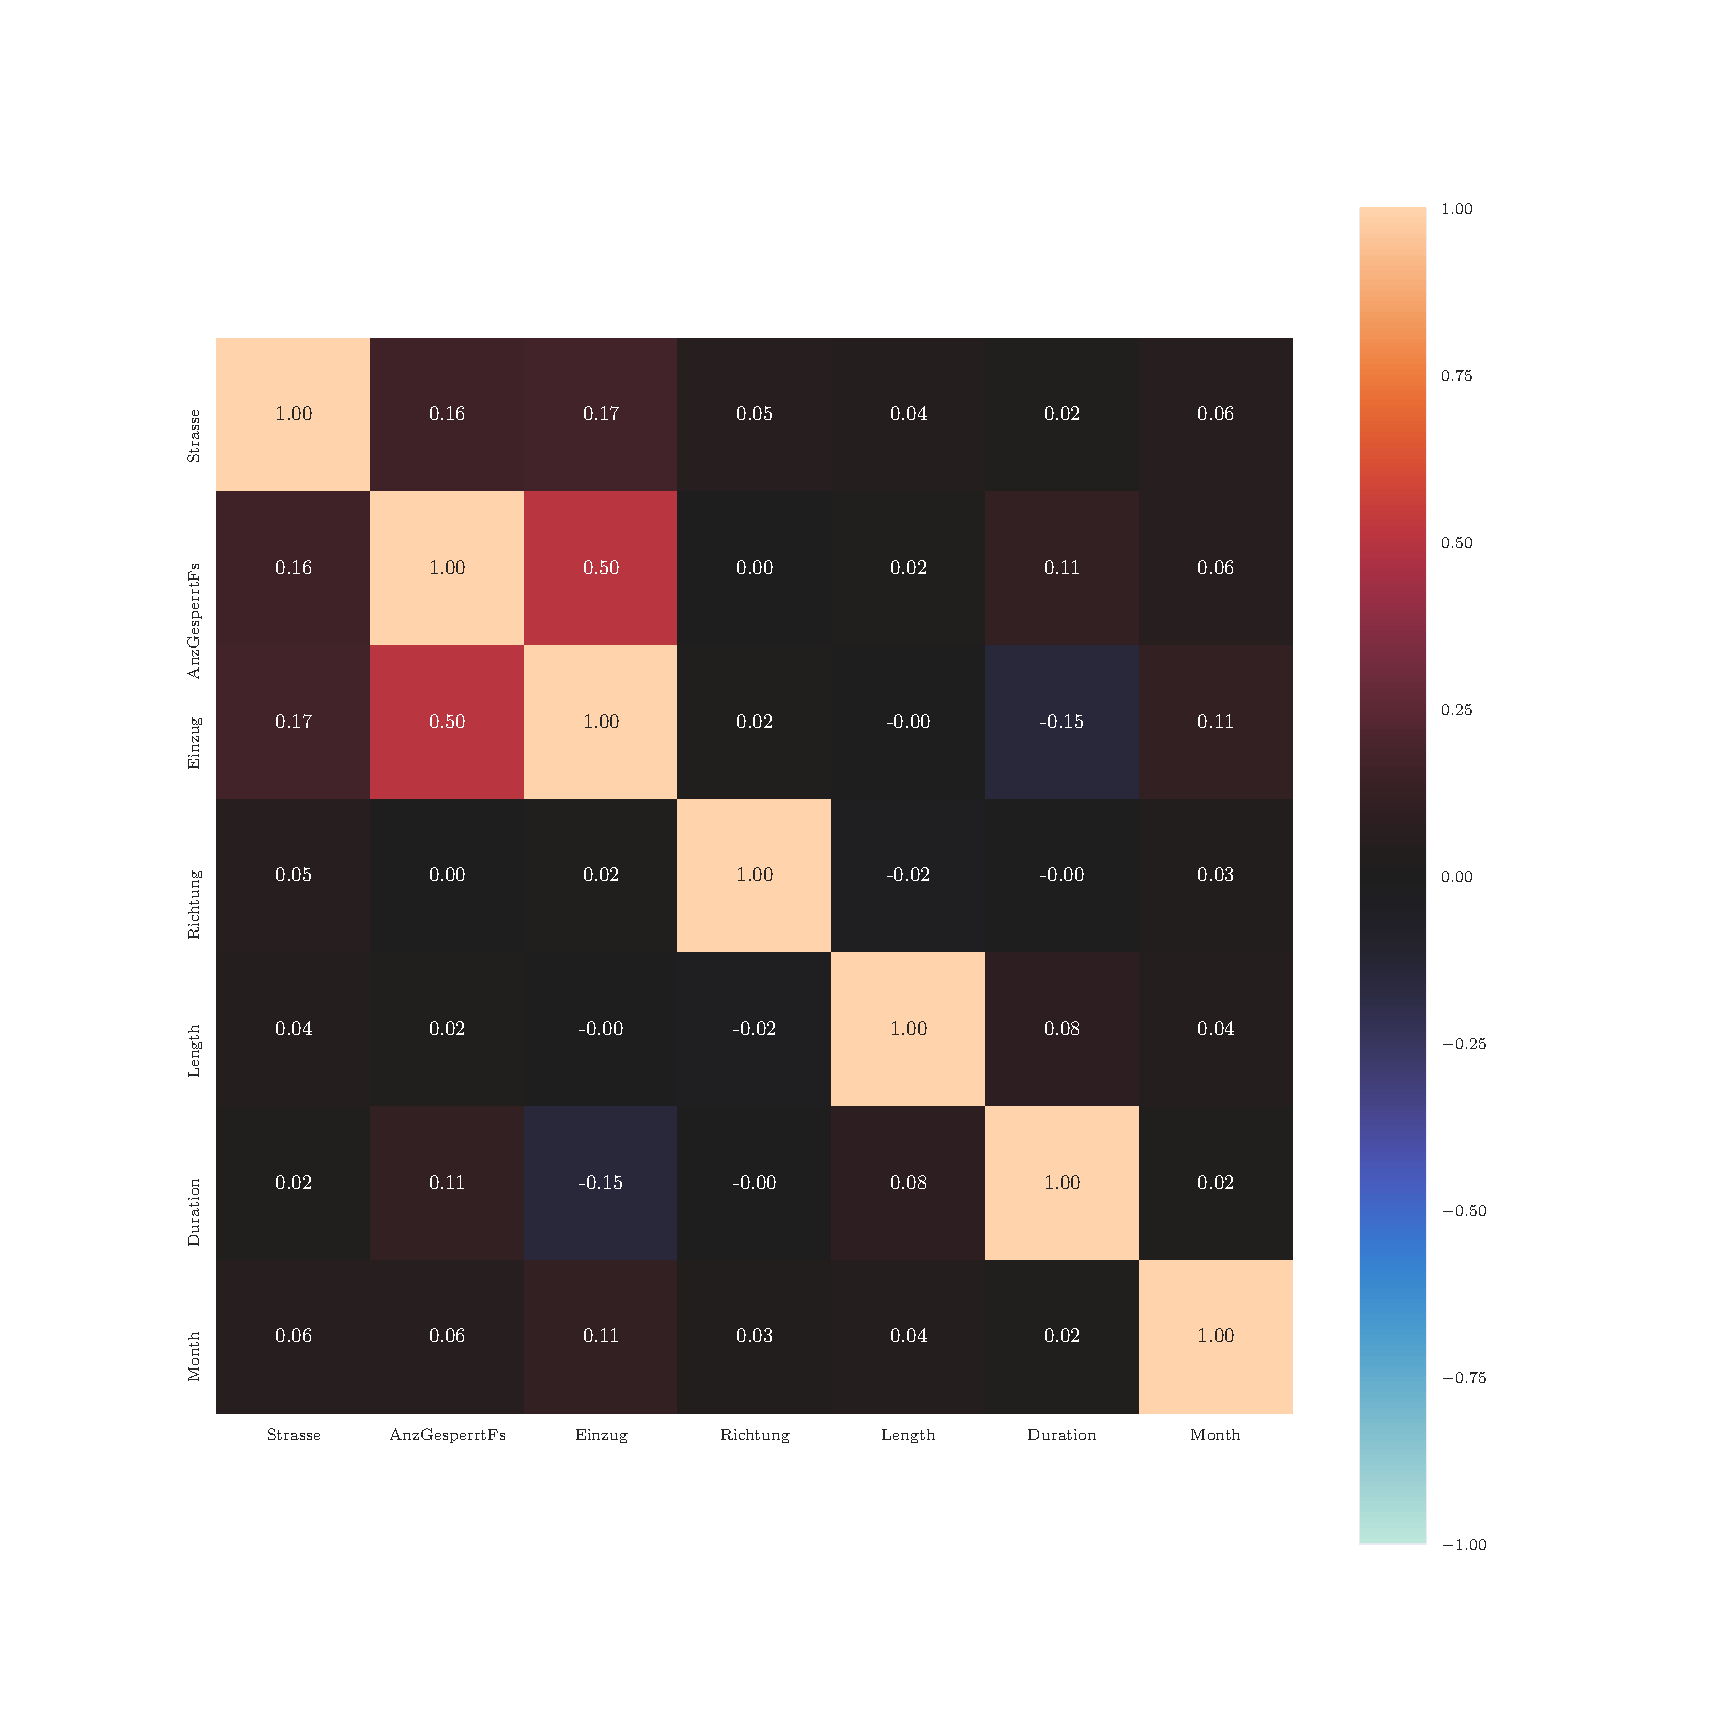
\includegraphics[scale=0.7, trim=0cm 2cm 0cm 0cm]{../CorrAnalysis/data/ArbIS/01_dataset/plots/arbis_dataset_corr_cramers}
    % 	\caption{Correlation matrix for ArbIS dataset, with Cramers's $V$}
    % 	\label{img:appendix_arbis_correlation_matrix_dataset_cramers}
    % \end{figure}
    % \restoregeometry
    
    % \newgeometry{left=1cm,right=1cm}
    % \begin{figure}[h]
    % 	\centering
    % 	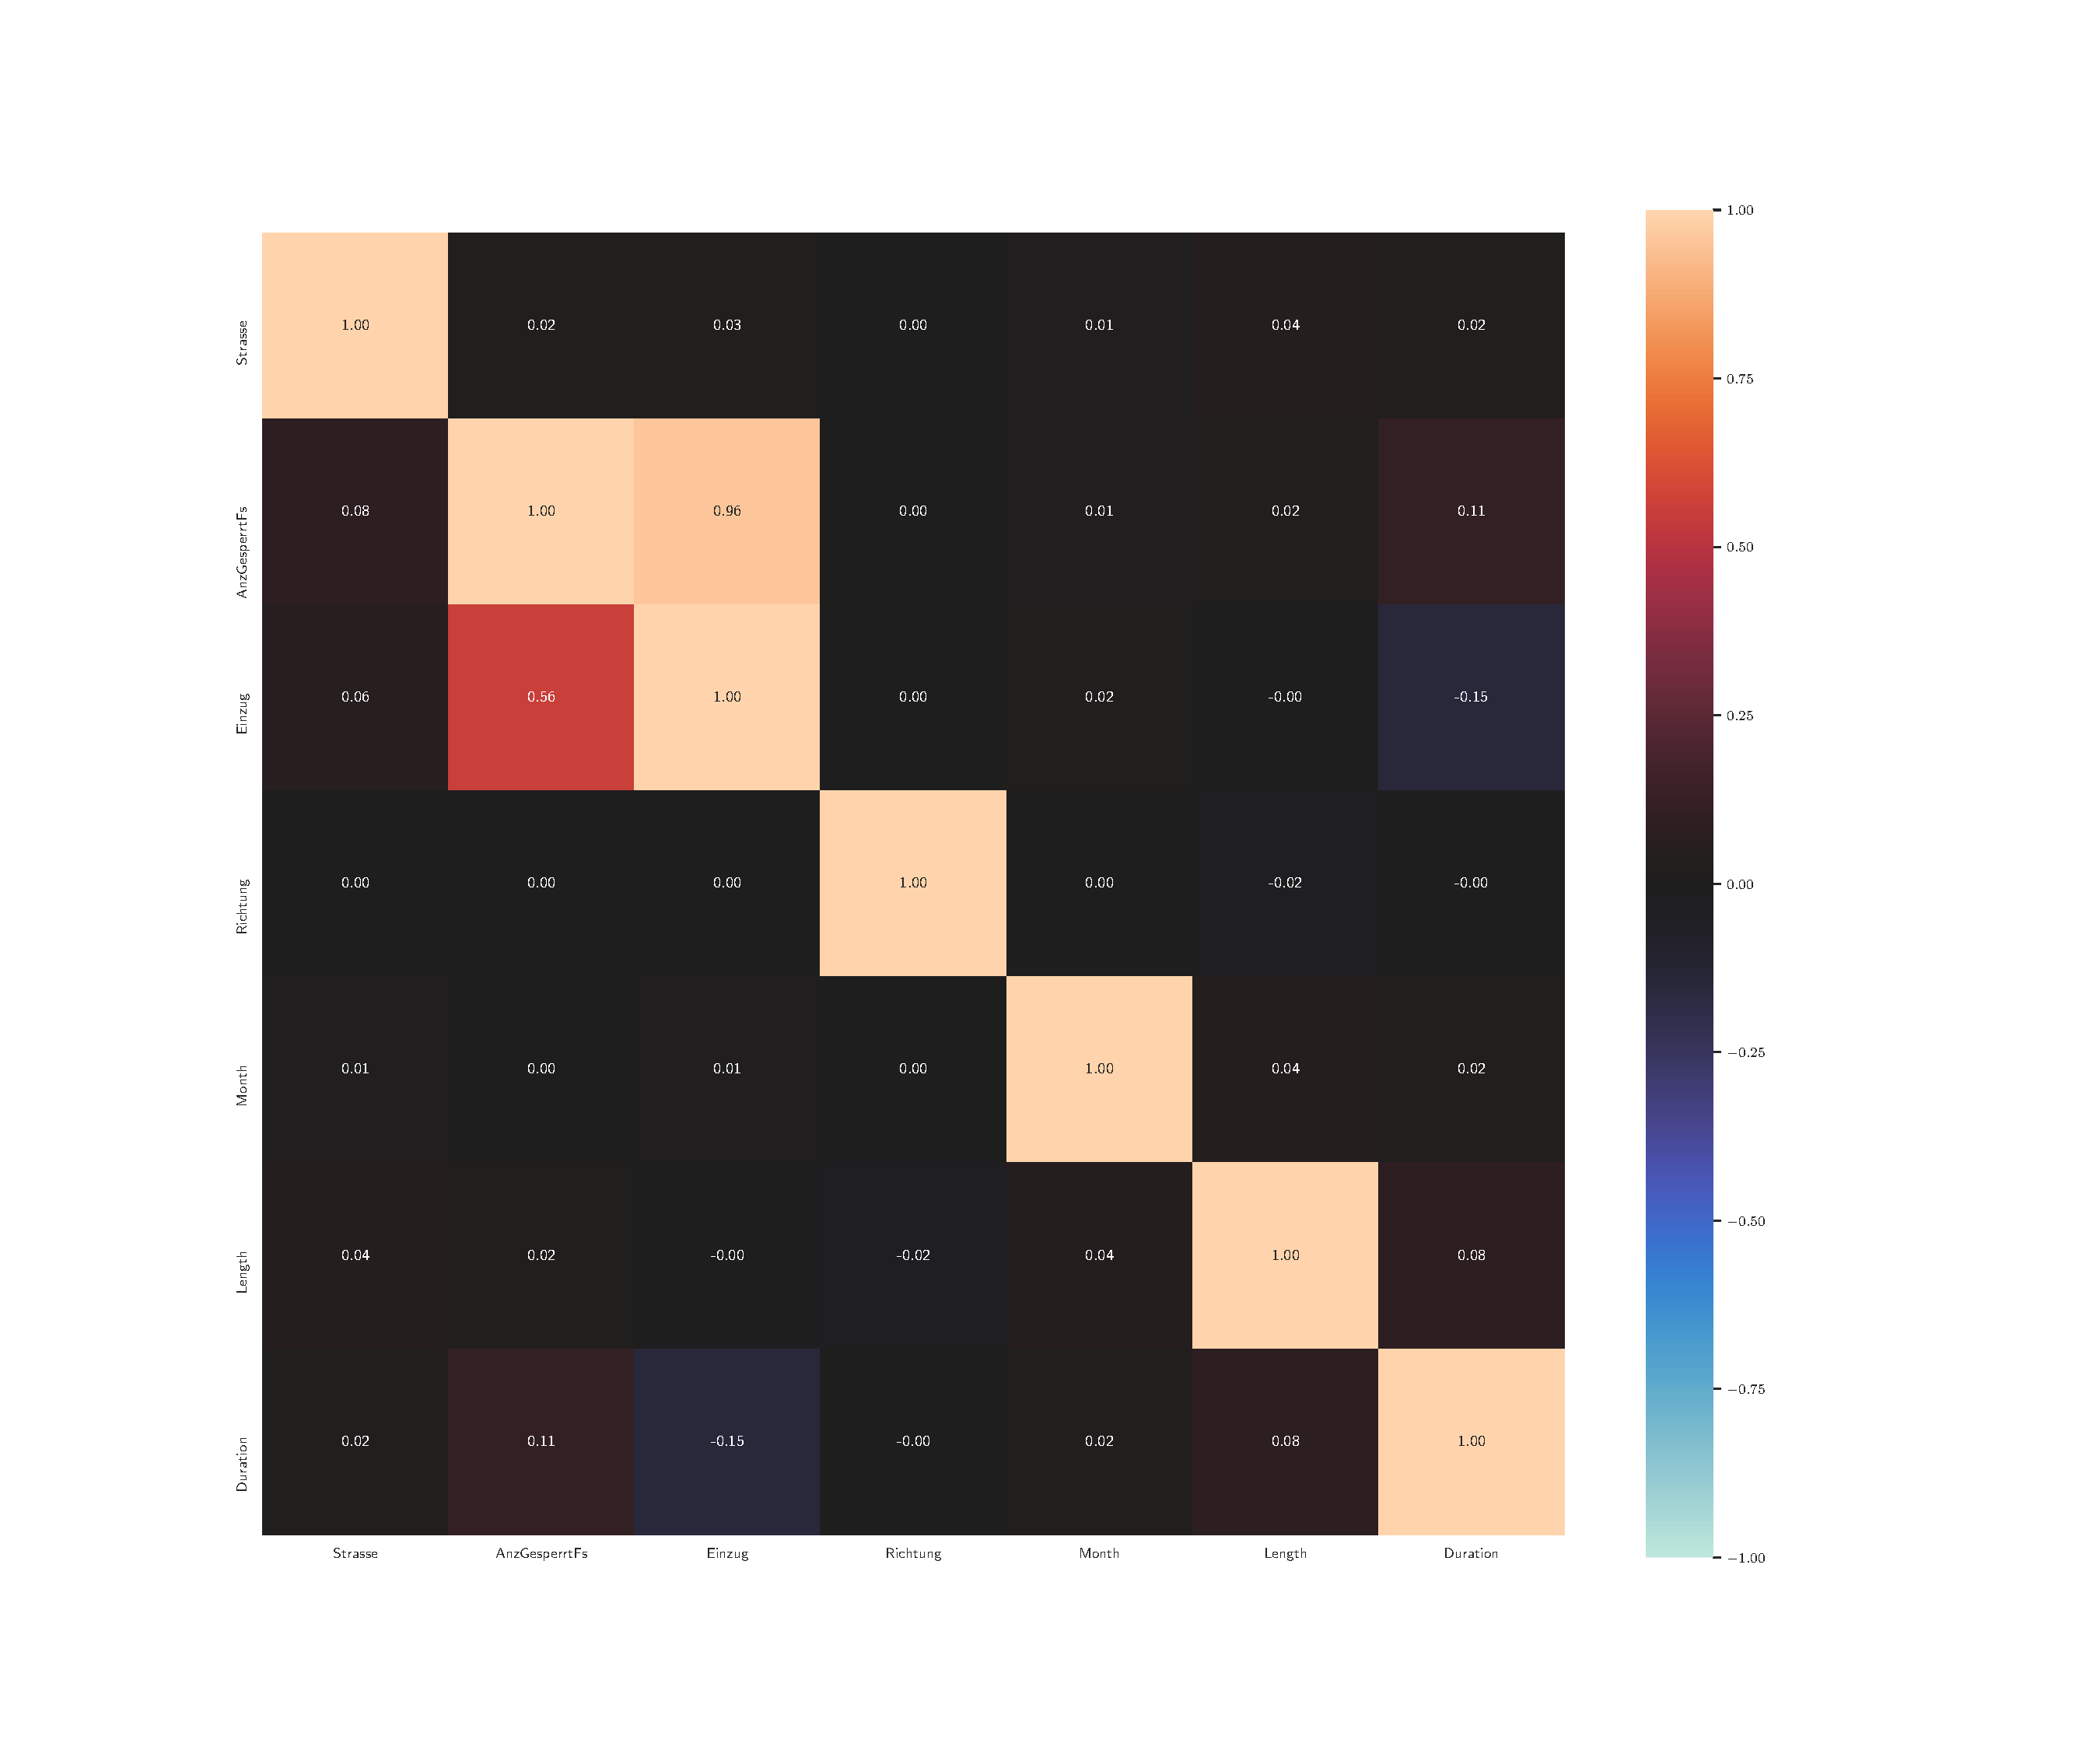
\includegraphics[scale=0.7, trim=0cm 2cm 0cm 0cm]{../CorrAnalysis/data/ArbIS/01_dataset/plots/arbis_dataset_corr_theils}
    % 	\caption{Correlation matrix for ArbIS dataset, with Theil's $U$}
    % 	\label{img:appendix_arbis_correlation_matrix_dataset_theils}
    % \end{figure}
    % \restoregeometry
    
    % ------- ArbIS Dataset - Tables --------
    \newgeometry{left=1cm,right=1cm}
    \begin{table}
    \setlength{\tabcolsep}{4pt}
    \centering
    \begin{tabular}{lrrrrrrr}
\toprule
{} &  Strasse &  AnzGesperrtFs &  Einzug &  Richtung &  Month &  Length &  Duration \\
\midrule
Strasse       &     1.00 &           0.16 &    0.17 &      0.05 &   0.06 &    0.04 &      0.02 \\
AnzGesperrtFs &     0.16 &           1.00 &    0.50 &      0.00 &   0.06 &    0.02 &      0.11 \\
Einzug        &     0.17 &           0.50 &    1.00 &      0.02 &   0.11 &   -0.00 &     -0.15 \\
Richtung      &     0.05 &           0.00 &    0.02 &      1.00 &   0.03 &   -0.02 &     -0.00 \\
Month         &     0.06 &           0.06 &    0.11 &      0.03 &   1.00 &    0.04 &      0.02 \\
Length        &     0.04 &           0.02 &   -0.00 &     -0.02 &   0.04 &    1.00 &      0.08 \\
Duration      &     0.02 &           0.11 &   -0.15 &     -0.00 &   0.02 &    0.08 &      1.00 \\
\bottomrule
\end{tabular}

    \caption{Correlation matrix for ArbIS dataset, with Cramer's $V$}
    \end{table}
    
    \begin{table}
    \setlength{\tabcolsep}{4pt}
    \centering
    \begin{tabular}{lrrrrrrr}
\toprule
{} &  Strasse &  AnzGesperrtFs &  Einzug &  Richtung &  Month &  Length &  Duration \\
\midrule
Strasse       &     1.00 &           0.02 &    0.03 &      0.00 &   0.01 &    0.04 &      0.02 \\
AnzGesperrtFs &     0.08 &           1.00 &    0.96 &      0.00 &   0.01 &    0.02 &      0.11 \\
Einzug        &     0.06 &           0.56 &    1.00 &      0.00 &   0.02 &   -0.00 &     -0.15 \\
Richtung      &     0.00 &           0.00 &    0.00 &      1.00 &   0.00 &   -0.02 &     -0.00 \\
Month         &     0.01 &           0.00 &    0.01 &      0.00 &   1.00 &    0.04 &      0.02 \\
Length        &     0.04 &           0.02 &   -0.00 &     -0.02 &   0.04 &    1.00 &      0.08 \\
Duration      &     0.02 &           0.11 &   -0.15 &     -0.00 &   0.02 &    0.08 &      1.00 \\
\bottomrule
\end{tabular}

    \caption{Correlation matrix for ArbIS dataset, with Theil's $U$}
    \end{table}
    
    \begin{table}
    \setlength{\tabcolsep}{4pt}
    \centering
    \begin{tabular}{lrrrrrrr}
\toprule
{} &  Strasse &  AnzGesperrtFs &  Einzug &  Richtung &  Length &  Duration &  Month \\
\midrule
Strasse       &      NaN &         0.0000 &  0.0000 &    0.0000 &  0.0000 &    0.0000 &    0.0 \\
AnzGesperrtFs &      0.0 &            NaN &  0.0000 &    0.2547 &  0.0000 &    0.0000 &    0.0 \\
Einzug        &      0.0 &         0.0000 &     NaN &    0.0000 &  0.0006 &    0.0000 &    0.0 \\
Richtung      &      0.0 &         0.2547 &  0.0000 &       NaN &  0.0000 &    0.0489 &    0.0 \\
Length        &      0.0 &         0.0000 &  0.0006 &    0.0000 &     NaN &    0.0000 &    0.0 \\
Duration      &      0.0 &         0.0000 &  0.0000 &    0.0489 &  0.0000 &       NaN &    0.0 \\
Month         &      0.0 &         0.0000 &  0.0000 &    0.0000 &  0.0000 &    0.0000 &    NaN \\
\bottomrule
\end{tabular}

    \caption{Significancy matrix for ArbIS dataset}
    \end{table}
    
    \begin{table}
    \setlength{\tabcolsep}{4pt}
    \centering
    \begin{tabular}{llllllll}
\toprule
{} & Strasse & AnzGesperrtFs &  Einzug &  Richtung &    Length &  Duration &   Month \\
\midrule
Strasse       &     NaN &           $V$ &     $V$ &       $V$ &    $\eta$ &    $\eta$ &     $V$ \\
AnzGesperrtFs &     $V$ &           NaN &     $V$ &       $V$ &    $\tau$ &    $\tau$ &     $V$ \\
Einzug        &     $V$ &           $V$ &     NaN &       $V$ &    $\tau$ &    $\tau$ &     $V$ \\
Richtung      &     $V$ &           $V$ &     $V$ &       NaN &  $r_{pq}$ &  $r_{pq}$ &     $V$ \\
Length        &  $\eta$ &        $\tau$ &  $\tau$ &  $r_{pq}$ &       NaN &       $r$ &  $\eta$ \\
Duration      &  $\eta$ &        $\tau$ &  $\tau$ &  $r_{pq}$ &       $r$ &       NaN &  $\eta$ \\
Month         &     $V$ &           $V$ &     $V$ &       $V$ &    $\eta$ &    $\eta$ &     NaN \\
\bottomrule
\end{tabular}

    \caption{Coefficient matrix for ArbIS dataset}
    \end{table}
    \restoregeometry
    
    % -------------------------------
    % ------- ArbIS Matched ---------
    % -------------------------------
    \tocless\section{ArbIS Matched Data}
    \label{appendix_ArbIS_matched}
    
    % ------- ArbIS Matched - Figures --------
    
    
    
    % ------- ArbIS Matched - Matrix --------
    % \newgeometry{left=1cm,right=1cm}
    % \begin{figure}[h]
    % 	\centering
    % 	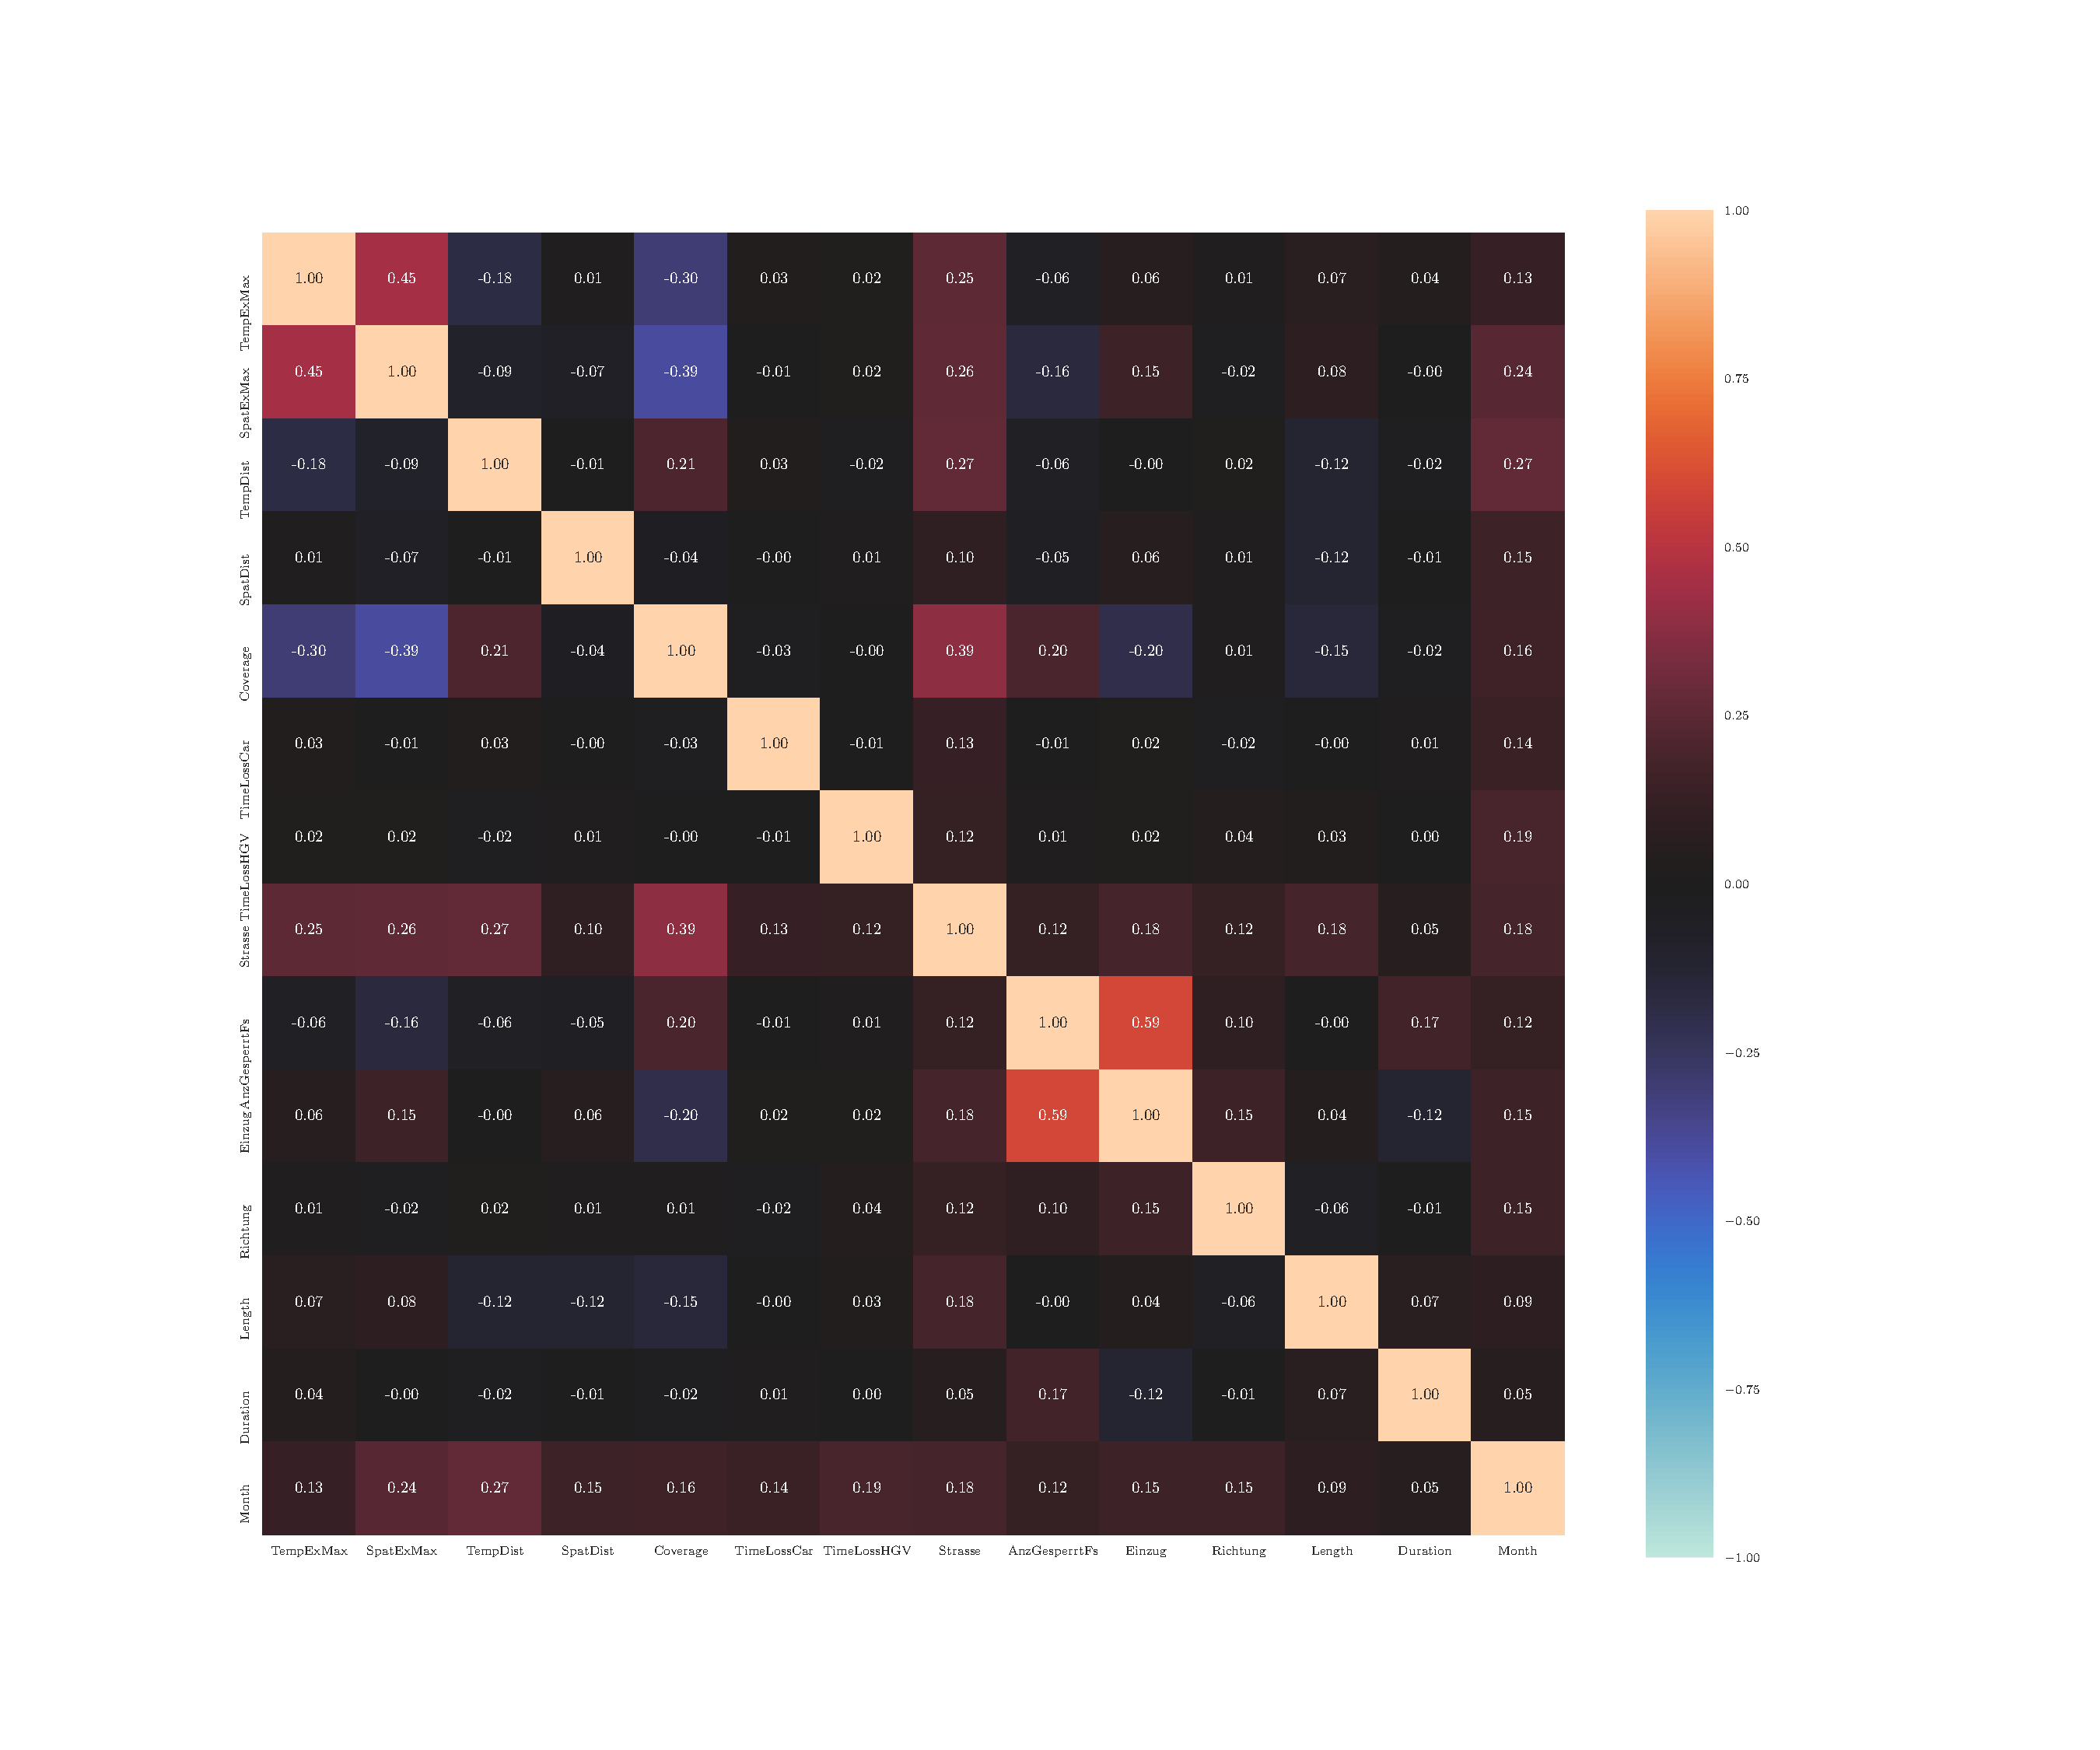
\includegraphics[scale=0.4, trim=0cm 2cm 0cm 0cm]{../CorrAnalysis/data/ArbIS/02_matched/plots/arbis_matched_corr_cramers}
    % 	\caption{Correlation matrix for ArbIS matched data, with Cramer's $V$}
    % 	\label{img:appendix_arbis_correlation_matrix_matched_cramers}
    % \end{figure}
    % \restoregeometry
    
    % \newgeometry{left=1cm,right=1cm}
    % \begin{figure}[h]
    % 	\centering
    % 	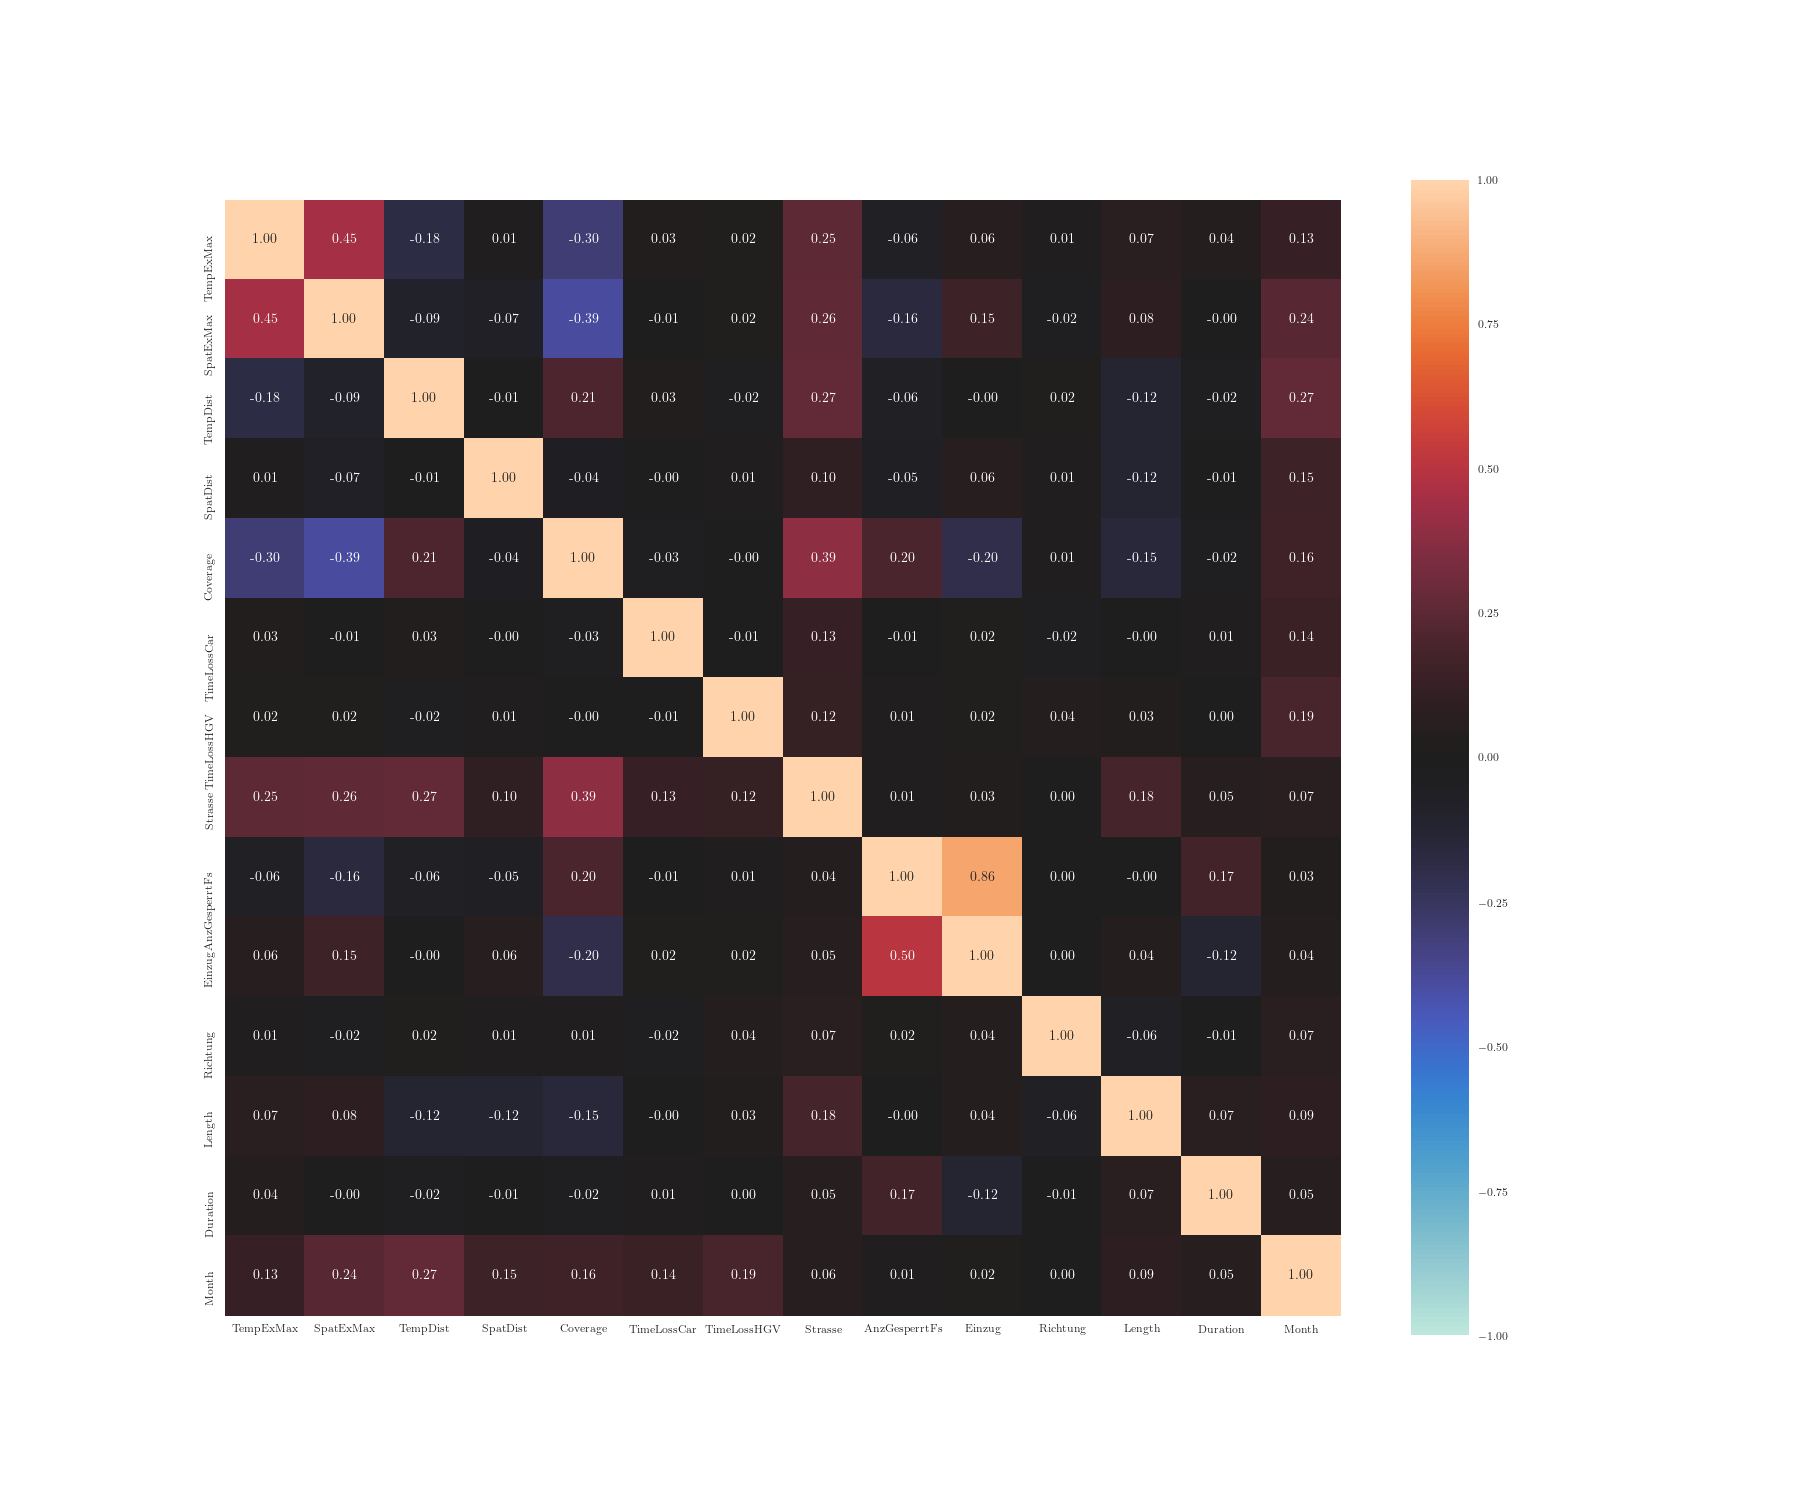
\includegraphics[scale=0.4, trim=0cm 2cm 0cm 0cm]{../CorrAnalysis/data/ArbIS/02_matched/plots/arbis_matched_corr_theils}
    % 	\caption{Correlation matrix for ArbIS matched data, with Theil's $U$}
    % 	\label{img:appendix_arbis_correlation_matrix_matched_theils}
    % \end{figure}
    % \restoregeometry
    
    % ------- ArbIS Matched - Tables --------
    \newgeometry{left=1cm,right=1cm,top=1cm}
    \begin{sidewaystable}
    \tiny
    \setlength{\tabcolsep}{4pt}
    \centering
    \begin{tabular}{lrrrrrrrrrrrrrrrr}
\toprule
{} &  TempMax &  TempAvg &  SpatMax &  SpatAvg &  TempDist &  SpatDist &  Coverage &  TLCar &  TLHGV &  Strasse &  AnzGesperrtFs &  Einzug &  Richtung &  Length &  Duration &  Month \\
\midrule
TempMax       &     1.00 &     0.77 &     0.44 &     0.50 &     -0.19 &     -0.03 &     -0.23 &   0.05 &  -0.02 &     0.24 &          -0.05 &    0.04 &      0.02 &    0.07 &      0.02 &   0.13 \\
TempAvg       &     0.77 &     1.00 &     0.11 &     0.42 &     -0.17 &     -0.00 &      0.19 &   0.04 &   0.03 &     0.19 &           0.05 &   -0.06 &      0.02 &    0.00 &      0.02 &   0.20 \\
SpatMax       &     0.44 &     0.11 &     1.00 &     0.46 &     -0.10 &     -0.07 &     -0.37 &  -0.06 &  -0.08 &     0.25 &          -0.15 &    0.13 &     -0.02 &    0.07 &     -0.01 &   0.24 \\
SpatAvg       &     0.50 &     0.42 &     0.46 &     1.00 &     -0.17 &     -0.12 &     -0.04 &  -0.00 &  -0.03 &     0.23 &          -0.07 &    0.05 &     -0.01 &    0.08 &     -0.00 &   0.14 \\
TempDist      &    -0.19 &    -0.17 &    -0.10 &    -0.17 &      1.00 &      0.07 &     -0.01 &   0.01 &   0.03 &     0.16 &          -0.03 &   -0.00 &      0.01 &   -0.06 &     -0.02 &   0.15 \\
SpatDist      &    -0.03 &    -0.00 &    -0.07 &    -0.12 &      0.07 &      1.00 &     -0.06 &   0.01 &   0.02 &     0.16 &          -0.06 &    0.08 &      0.03 &   -0.11 &     -0.01 &   0.14 \\
Coverage      &    -0.23 &     0.19 &    -0.37 &    -0.04 &     -0.01 &     -0.06 &      1.00 &  -0.05 &  -0.02 &     0.41 &           0.18 &   -0.17 &     -0.00 &   -0.11 &     -0.01 &   0.24 \\
TLCar         &     0.05 &     0.04 &    -0.06 &    -0.00 &      0.01 &      0.01 &     -0.05 &   1.00 &   0.09 &     0.14 &          -0.03 &    0.01 &     -0.02 &    0.02 &      0.00 &   0.14 \\
TLHGV         &    -0.02 &     0.03 &    -0.08 &    -0.03 &      0.03 &      0.02 &     -0.02 &   0.09 &   1.00 &     0.16 &          -0.01 &   -0.00 &      0.03 &   -0.00 &      0.02 &   0.13 \\
Strasse       &     0.24 &     0.19 &     0.25 &     0.23 &      0.16 &      0.16 &      0.41 &   0.14 &   0.16 &     1.00 &           0.13 &    0.17 &      0.13 &    0.17 &      0.07 &   0.18 \\
AnzGesperrtFs &    -0.05 &     0.05 &    -0.15 &    -0.07 &     -0.03 &     -0.06 &      0.18 &  -0.03 &  -0.01 &     0.13 &           1.00 &    0.50 &      0.18 &   -0.03 &      0.14 &   0.11 \\
Einzug        &     0.04 &    -0.06 &     0.13 &     0.05 &     -0.00 &      0.08 &     -0.17 &   0.01 &  -0.00 &     0.17 &           0.50 &    1.00 &      0.14 &    0.03 &     -0.12 &   0.14 \\
Richtung      &     0.02 &     0.02 &    -0.02 &    -0.01 &      0.01 &      0.03 &     -0.00 &  -0.02 &   0.03 &     0.13 &           0.18 &    0.14 &      1.00 &   -0.05 &     -0.07 &   0.14 \\
Length        &     0.07 &     0.00 &     0.07 &     0.08 &     -0.06 &     -0.11 &     -0.11 &   0.02 &  -0.00 &     0.17 &          -0.03 &    0.03 &     -0.05 &    1.00 &      0.07 &   0.08 \\
Duration      &     0.02 &     0.02 &    -0.01 &    -0.00 &     -0.02 &     -0.01 &     -0.01 &   0.00 &   0.02 &     0.07 &           0.14 &   -0.12 &     -0.07 &    0.07 &      1.00 &   0.05 \\
Month         &     0.13 &     0.20 &     0.24 &     0.14 &      0.15 &      0.14 &      0.24 &   0.14 &   0.13 &     0.18 &           0.11 &    0.14 &      0.14 &    0.08 &      0.05 &   1.00 \\
\bottomrule
\end{tabular}

    \caption{Correlation matrix for ArbIS matched data, with Cramer's $V$}
    \end{sidewaystable}
    
    \begin{sidewaystable}
    \tiny
    \setlength{\tabcolsep}{4pt}
    \centering
    \begin{tabular}{lrrrrrrrrrrrrrr}
\toprule
{} &  TempExMax &  SpatExMax &  TempDist &  SpatDist &  Coverage &  TimeLossCar &  TimeLossHGV &  Strasse &  AnzGesperrtFs &  Einzug &  Richtung &  Length &  Duration &  Month \\
\midrule
TempExMax     &       1.00 &       0.45 &     -0.18 &      0.01 &     -0.30 &         0.03 &         0.02 &     0.25 &          -0.06 &    0.06 &      0.01 &    0.07 &      0.04 &   0.13 \\
SpatExMax     &       0.45 &       1.00 &     -0.09 &     -0.07 &     -0.39 &        -0.01 &         0.02 &     0.26 &          -0.16 &    0.15 &     -0.02 &    0.08 &     -0.00 &   0.24 \\
TempDist      &      -0.18 &      -0.09 &      1.00 &     -0.01 &      0.21 &         0.03 &        -0.02 &     0.27 &          -0.06 &   -0.00 &      0.02 &   -0.12 &     -0.02 &   0.27 \\
SpatDist      &       0.01 &      -0.07 &     -0.01 &      1.00 &     -0.04 &        -0.00 &         0.01 &     0.10 &          -0.05 &    0.06 &      0.01 &   -0.12 &     -0.01 &   0.15 \\
Coverage      &      -0.30 &      -0.39 &      0.21 &     -0.04 &      1.00 &        -0.03 &        -0.00 &     0.39 &           0.20 &   -0.20 &      0.01 &   -0.15 &     -0.02 &   0.16 \\
TimeLossCar   &       0.03 &      -0.01 &      0.03 &     -0.00 &     -0.03 &         1.00 &        -0.01 &     0.13 &          -0.01 &    0.02 &     -0.02 &   -0.00 &      0.01 &   0.14 \\
TimeLossHGV   &       0.02 &       0.02 &     -0.02 &      0.01 &     -0.00 &        -0.01 &         1.00 &     0.12 &           0.01 &    0.02 &      0.04 &    0.03 &      0.00 &   0.19 \\
Strasse       &       0.25 &       0.26 &      0.27 &      0.10 &      0.39 &         0.13 &         0.12 &     1.00 &           0.01 &    0.03 &      0.00 &    0.18 &      0.05 &   0.07 \\
AnzGesperrtFs &      -0.06 &      -0.16 &     -0.06 &     -0.05 &      0.20 &        -0.01 &         0.01 &     0.04 &           1.00 &    0.86 &      0.00 &   -0.00 &      0.17 &   0.03 \\
Einzug        &       0.06 &       0.15 &     -0.00 &      0.06 &     -0.20 &         0.02 &         0.02 &     0.05 &           0.50 &    1.00 &      0.00 &    0.04 &     -0.12 &   0.04 \\
Richtung      &       0.01 &      -0.02 &      0.02 &      0.01 &      0.01 &        -0.02 &         0.04 &     0.07 &           0.02 &    0.04 &      1.00 &   -0.06 &     -0.01 &   0.07 \\
Length        &       0.07 &       0.08 &     -0.12 &     -0.12 &     -0.15 &        -0.00 &         0.03 &     0.18 &          -0.00 &    0.04 &     -0.06 &    1.00 &      0.07 &   0.09 \\
Duration      &       0.04 &      -0.00 &     -0.02 &     -0.01 &     -0.02 &         0.01 &         0.00 &     0.05 &           0.17 &   -0.12 &     -0.01 &    0.07 &      1.00 &   0.05 \\
Month         &       0.13 &       0.24 &      0.27 &      0.15 &      0.16 &         0.14 &         0.19 &     0.06 &           0.01 &    0.02 &      0.00 &    0.09 &      0.05 &   1.00 \\
\bottomrule
\end{tabular}

    \caption{Correlation matrix for ArbIS matched data, with Theil's $U$}
    \end{sidewaystable}
    
    \begin{sidewaystable}
    \tiny
    \setlength{\tabcolsep}{4pt}
    \centering
    \begin{tabular}{lrrrrrrrrrrrrrr}
\toprule
{} &  TempExMax &  SpatExMax &  TempDist &  SpatDist &  Coverage &  TimeLossCar &  TimeLossHGV &  Strasse &  AnzGesperrtFs &  Einzug &  Richtung &  Length &  Duration &  Month \\
\midrule
TempExMax     &        NaN &     0.0000 &    0.0000 &    0.4231 &    0.0000 &       0.1425 &       0.3315 &   0.0000 &         0.0000 &  0.0000 &    0.4581 &  0.0004 &    0.0544 &    0.0 \\
SpatExMax     &     0.0000 &        NaN &    0.0000 &    0.0001 &    0.0000 &       0.6088 &       0.1853 &   0.0000 &         0.0000 &  0.0000 &    0.2429 &  0.0000 &    0.8016 &    0.0 \\
TempDist      &     0.0000 &     0.0000 &       NaN &    0.5160 &    0.0000 &       0.1027 &       0.3490 &   0.0000 &         0.0003 &  0.7686 &    0.3701 &  0.0000 &    0.2463 &    0.0 \\
SpatDist      &     0.4231 &     0.0001 &    0.5160 &       NaN &    0.0258 &       0.9198 &       0.7391 &   0.0000 &         0.0074 &  0.0009 &    0.6300 &  0.0000 &    0.5061 &    0.0 \\
Coverage      &     0.0000 &     0.0000 &    0.0000 &    0.0258 &       NaN &       0.1132 &       0.8785 &   0.0000 &         0.0000 &  0.0000 &    0.7317 &  0.0000 &    0.2080 &    0.0 \\
TimeLossCar   &     0.1425 &     0.6088 &    0.1027 &    0.9198 &    0.1132 &          NaN &       0.4229 &   0.0000 &         0.3282 &  0.0993 &    0.3305 &  0.9555 &    0.4984 &    0.0 \\
TimeLossHGV   &     0.3315 &     0.1853 &    0.3490 &    0.7391 &    0.8785 &       0.4229 &          NaN &   0.0000 &         0.3505 &  0.1101 &    0.0338 &  0.1641 &    0.8675 &    0.0 \\
Strasse       &     0.0000 &     0.0000 &    0.0000 &    0.0000 &    0.0000 &       0.0000 &       0.0000 &      NaN &         0.0000 &  0.0000 &    0.0002 &  0.0000 &    0.0000 &    0.0 \\
AnzGesperrtFs &     0.0000 &     0.0000 &    0.0003 &    0.0074 &    0.0000 &       0.3282 &       0.3505 &   0.0000 &            NaN &  0.0000 &    0.0000 &  0.8918 &    0.0000 &    0.0 \\
Einzug        &     0.0000 &     0.0000 &    0.7686 &    0.0009 &    0.0000 &       0.0993 &       0.1101 &   0.0000 &         0.0000 &     NaN &    0.0000 &  0.0069 &    0.0000 &    0.0 \\
Richtung      &     0.4581 &     0.2429 &    0.3701 &    0.6300 &    0.7317 &       0.3305 &       0.0338 &   0.0002 &         0.0000 &  0.0000 &       NaN &  0.0017 &    0.7496 &    0.0 \\
Length        &     0.0004 &     0.0000 &    0.0000 &    0.0000 &    0.0000 &       0.9555 &       0.1641 &   0.0000 &         0.8918 &  0.0069 &    0.0017 &     NaN &    0.0001 &    0.0 \\
Duration      &     0.0544 &     0.8016 &    0.2463 &    0.5061 &    0.2080 &       0.4984 &       0.8675 &   0.0000 &         0.0000 &  0.0000 &    0.7496 &  0.0001 &       NaN &    0.0 \\
Month         &     0.0000 &     0.0000 &    0.0000 &    0.0000 &    0.0000 &       0.0000 &       0.0000 &   0.0000 &         0.0000 &  0.0000 &    0.0000 &  0.0000 &    0.0000 &    NaN \\
\bottomrule
\end{tabular}

    \caption{Significancy matrix for ArbIS matched data}
    \end{sidewaystable}

    \begin{sidewaystable}
    \tiny
    \setlength{\tabcolsep}{4pt}
    \centering
    \begin{tabular}{lllllllllllllll}
\toprule
{} &       TempExMax &       SpatExMax &        TempDist &        SpatDist &        Coverage &     TimeLossCar &     TimeLossHGV &     Strasse & AnzGesperrtFs &      Einzug &        Richtung &          Length &        Duration &       Month \\
\midrule
TempExMax     &             NaN &         Pearson &         Pearson &         Pearson &         Pearson &         Pearson &         Pearson &         Eta &       Kendall &     Kendall &  Point Biserial &         Pearson &         Pearson &         Eta \\
SpatExMax     &         Pearson &             NaN &         Pearson &         Pearson &         Pearson &         Pearson &         Pearson &         Eta &       Kendall &     Kendall &  Point Biserial &         Pearson &         Pearson &         Eta \\
TempDist      &         Pearson &         Pearson &             NaN &         Pearson &         Pearson &         Pearson &         Pearson &         Eta &       Kendall &     Kendall &  Point Biserial &         Pearson &         Pearson &         Eta \\
SpatDist      &         Pearson &         Pearson &         Pearson &             NaN &         Pearson &         Pearson &         Pearson &         Eta &       Kendall &     Kendall &  Point Biserial &         Pearson &         Pearson &         Eta \\
Coverage      &         Pearson &         Pearson &         Pearson &         Pearson &             NaN &         Pearson &         Pearson &         Eta &       Kendall &     Kendall &  Point Biserial &         Pearson &         Pearson &         Eta \\
TimeLossCar   &         Pearson &         Pearson &         Pearson &         Pearson &         Pearson &             NaN &         Pearson &         Eta &       Kendall &     Kendall &  Point Biserial &         Pearson &         Pearson &         Eta \\
TimeLossHGV   &         Pearson &         Pearson &         Pearson &         Pearson &         Pearson &         Pearson &             NaN &         Eta &       Kendall &     Kendall &  Point Biserial &         Pearson &         Pearson &         Eta \\
Strasse       &             Eta &             Eta &             Eta &             Eta &             Eta &             Eta &             Eta &         NaN &    Cramer's V &  Cramer's V &      Cramer's V &             Eta &             Eta &  Cramer's V \\
AnzGesperrtFs &         Kendall &         Kendall &         Kendall &         Kendall &         Kendall &         Kendall &         Kendall &  Cramer's V &           NaN &  Cramer's V &      Cramer's V &         Kendall &         Kendall &  Cramer's V \\
Einzug        &         Kendall &         Kendall &         Kendall &         Kendall &         Kendall &         Kendall &         Kendall &  Cramer's V &    Cramer's V &         NaN &      Cramer's V &         Kendall &         Kendall &  Cramer's V \\
Richtung      &  Point Biserial &  Point Biserial &  Point Biserial &  Point Biserial &  Point Biserial &  Point Biserial &  Point Biserial &  Cramer's V &    Cramer's V &  Cramer's V &             NaN &  Point Biserial &  Point Biserial &  Cramer's V \\
Length        &         Pearson &         Pearson &         Pearson &         Pearson &         Pearson &         Pearson &         Pearson &         Eta &       Kendall &     Kendall &  Point Biserial &             NaN &         Pearson &         Eta \\
Duration      &         Pearson &         Pearson &         Pearson &         Pearson &         Pearson &         Pearson &         Pearson &         Eta &       Kendall &     Kendall &  Point Biserial &         Pearson &             NaN &         Eta \\
Month         &             Eta &             Eta &             Eta &             Eta &             Eta &             Eta &             Eta &  Cramer's V &    Cramer's V &  Cramer's V &      Cramer's V &             Eta &             Eta &         NaN \\
\bottomrule
\end{tabular}

    \caption{Coefficient matrix for ArbIS matched data}
    \end{sidewaystable}
    
    % -------------------------------------
    % ------- Source Code Appendix --------
    % -------------------------------------
    \chapter{Source Code}
    
    % -------------------------------------
    % ------- Cluster Algorithm ---------
    \tocless\section{CongstatsClusterAlgorithm}
    %\label{appendix_TODO}
    %\begingroup
    %    \fontsize{2pt}{6pt}\selectfont
    %		\lstinputlisting[language=java]{../CongEvaluation/congestion/clustering/CongstatsClusterAlgorithm.java}
    %\endgroup
    
    % ------------------------------
    % ------- Shaping Algorithm ---------
    
    % -------------------------------
    % ------- Matching Algorithm ---------
    
    % -----------------------------------
    % ------- Processing Export ---------
    
    % ---------------------------------
    % ------- Processing Corr ---------
    
    \end{appendices}
    
